% Options for packages loaded elsewhere
\PassOptionsToPackage{unicode}{hyperref}
\PassOptionsToPackage{hyphens}{url}
\PassOptionsToPackage{dvipsnames,svgnames,x11names}{xcolor}
%
\documentclass[
  11pt,
  letterpaper,
  DIV=11,
  numbers=noendperiod]{scrreprt}

\usepackage{amsmath,amssymb}
\usepackage{iftex}
\ifPDFTeX
  \usepackage[T1]{fontenc}
  \usepackage[utf8]{inputenc}
  \usepackage{textcomp} % provide euro and other symbols
\else % if luatex or xetex
  \usepackage{unicode-math}
  \defaultfontfeatures{Scale=MatchLowercase}
  \defaultfontfeatures[\rmfamily]{Ligatures=TeX,Scale=1}
\fi
\usepackage{lmodern}
\ifPDFTeX\else  
    % xetex/luatex font selection
\fi
% Use upquote if available, for straight quotes in verbatim environments
\IfFileExists{upquote.sty}{\usepackage{upquote}}{}
\IfFileExists{microtype.sty}{% use microtype if available
  \usepackage[]{microtype}
  \UseMicrotypeSet[protrusion]{basicmath} % disable protrusion for tt fonts
}{}
\makeatletter
\@ifundefined{KOMAClassName}{% if non-KOMA class
  \IfFileExists{parskip.sty}{%
    \usepackage{parskip}
  }{% else
    \setlength{\parindent}{0pt}
    \setlength{\parskip}{6pt plus 2pt minus 1pt}}
}{% if KOMA class
  \KOMAoptions{parskip=half}}
\makeatother
\usepackage{xcolor}
\usepackage[margin=1in]{geometry}
\setlength{\emergencystretch}{3em} % prevent overfull lines
\setcounter{secnumdepth}{5}
% Make \paragraph and \subparagraph free-standing
\ifx\paragraph\undefined\else
  \let\oldparagraph\paragraph
  \renewcommand{\paragraph}[1]{\oldparagraph{#1}\mbox{}}
\fi
\ifx\subparagraph\undefined\else
  \let\oldsubparagraph\subparagraph
  \renewcommand{\subparagraph}[1]{\oldsubparagraph{#1}\mbox{}}
\fi

\usepackage{color}
\usepackage{fancyvrb}
\newcommand{\VerbBar}{|}
\newcommand{\VERB}{\Verb[commandchars=\\\{\}]}
\DefineVerbatimEnvironment{Highlighting}{Verbatim}{commandchars=\\\{\}}
% Add ',fontsize=\small' for more characters per line
\usepackage{framed}
\definecolor{shadecolor}{RGB}{241,243,245}
\newenvironment{Shaded}{\begin{snugshade}}{\end{snugshade}}
\newcommand{\AlertTok}[1]{\textcolor[rgb]{0.68,0.00,0.00}{#1}}
\newcommand{\AnnotationTok}[1]{\textcolor[rgb]{0.37,0.37,0.37}{#1}}
\newcommand{\AttributeTok}[1]{\textcolor[rgb]{0.40,0.45,0.13}{#1}}
\newcommand{\BaseNTok}[1]{\textcolor[rgb]{0.68,0.00,0.00}{#1}}
\newcommand{\BuiltInTok}[1]{\textcolor[rgb]{0.00,0.23,0.31}{#1}}
\newcommand{\CharTok}[1]{\textcolor[rgb]{0.13,0.47,0.30}{#1}}
\newcommand{\CommentTok}[1]{\textcolor[rgb]{0.37,0.37,0.37}{#1}}
\newcommand{\CommentVarTok}[1]{\textcolor[rgb]{0.37,0.37,0.37}{\textit{#1}}}
\newcommand{\ConstantTok}[1]{\textcolor[rgb]{0.56,0.35,0.01}{#1}}
\newcommand{\ControlFlowTok}[1]{\textcolor[rgb]{0.00,0.23,0.31}{#1}}
\newcommand{\DataTypeTok}[1]{\textcolor[rgb]{0.68,0.00,0.00}{#1}}
\newcommand{\DecValTok}[1]{\textcolor[rgb]{0.68,0.00,0.00}{#1}}
\newcommand{\DocumentationTok}[1]{\textcolor[rgb]{0.37,0.37,0.37}{\textit{#1}}}
\newcommand{\ErrorTok}[1]{\textcolor[rgb]{0.68,0.00,0.00}{#1}}
\newcommand{\ExtensionTok}[1]{\textcolor[rgb]{0.00,0.23,0.31}{#1}}
\newcommand{\FloatTok}[1]{\textcolor[rgb]{0.68,0.00,0.00}{#1}}
\newcommand{\FunctionTok}[1]{\textcolor[rgb]{0.28,0.35,0.67}{#1}}
\newcommand{\ImportTok}[1]{\textcolor[rgb]{0.00,0.46,0.62}{#1}}
\newcommand{\InformationTok}[1]{\textcolor[rgb]{0.37,0.37,0.37}{#1}}
\newcommand{\KeywordTok}[1]{\textcolor[rgb]{0.00,0.23,0.31}{#1}}
\newcommand{\NormalTok}[1]{\textcolor[rgb]{0.00,0.23,0.31}{#1}}
\newcommand{\OperatorTok}[1]{\textcolor[rgb]{0.37,0.37,0.37}{#1}}
\newcommand{\OtherTok}[1]{\textcolor[rgb]{0.00,0.23,0.31}{#1}}
\newcommand{\PreprocessorTok}[1]{\textcolor[rgb]{0.68,0.00,0.00}{#1}}
\newcommand{\RegionMarkerTok}[1]{\textcolor[rgb]{0.00,0.23,0.31}{#1}}
\newcommand{\SpecialCharTok}[1]{\textcolor[rgb]{0.37,0.37,0.37}{#1}}
\newcommand{\SpecialStringTok}[1]{\textcolor[rgb]{0.13,0.47,0.30}{#1}}
\newcommand{\StringTok}[1]{\textcolor[rgb]{0.13,0.47,0.30}{#1}}
\newcommand{\VariableTok}[1]{\textcolor[rgb]{0.07,0.07,0.07}{#1}}
\newcommand{\VerbatimStringTok}[1]{\textcolor[rgb]{0.13,0.47,0.30}{#1}}
\newcommand{\WarningTok}[1]{\textcolor[rgb]{0.37,0.37,0.37}{\textit{#1}}}

\providecommand{\tightlist}{%
  \setlength{\itemsep}{0pt}\setlength{\parskip}{0pt}}\usepackage{longtable,booktabs,array}
\usepackage{calc} % for calculating minipage widths
% Correct order of tables after \paragraph or \subparagraph
\usepackage{etoolbox}
\makeatletter
\patchcmd\longtable{\par}{\if@noskipsec\mbox{}\fi\par}{}{}
\makeatother
% Allow footnotes in longtable head/foot
\IfFileExists{footnotehyper.sty}{\usepackage{footnotehyper}}{\usepackage{footnote}}
\makesavenoteenv{longtable}
\usepackage{graphicx}
\makeatletter
\def\maxwidth{\ifdim\Gin@nat@width>\linewidth\linewidth\else\Gin@nat@width\fi}
\def\maxheight{\ifdim\Gin@nat@height>\textheight\textheight\else\Gin@nat@height\fi}
\makeatother
% Scale images if necessary, so that they will not overflow the page
% margins by default, and it is still possible to overwrite the defaults
% using explicit options in \includegraphics[width, height, ...]{}
\setkeys{Gin}{width=\maxwidth,height=\maxheight,keepaspectratio}
% Set default figure placement to htbp
\makeatletter
\def\fps@figure{htbp}
\makeatother

\usepackage{booktabs}
\usepackage{caption}
\usepackage{longtable}
\usepackage{colortbl}
\usepackage{array}
\KOMAoption{captions}{tableheading}
\usepackage{graphicx}
\usepackage{fontspec}
\setmainfont{Times New Roman}
\usepackage{geometry}
\pagestyle{empty}
\makeatletter
\@ifpackageloaded{bookmark}{}{\usepackage{bookmark}}
\makeatother
\makeatletter
\@ifpackageloaded{caption}{}{\usepackage{caption}}
\AtBeginDocument{%
\ifdefined\contentsname
  \renewcommand*\contentsname{Table of contents}
\else
  \newcommand\contentsname{Table of contents}
\fi
\ifdefined\listfigurename
  \renewcommand*\listfigurename{List of Figures}
\else
  \newcommand\listfigurename{List of Figures}
\fi
\ifdefined\listtablename
  \renewcommand*\listtablename{List of Tables}
\else
  \newcommand\listtablename{List of Tables}
\fi
\ifdefined\figurename
  \renewcommand*\figurename{Figure}
\else
  \newcommand\figurename{Figure}
\fi
\ifdefined\tablename
  \renewcommand*\tablename{Table}
\else
  \newcommand\tablename{Table}
\fi
}
\@ifpackageloaded{float}{}{\usepackage{float}}
\floatstyle{ruled}
\@ifundefined{c@chapter}{\newfloat{codelisting}{h}{lop}}{\newfloat{codelisting}{h}{lop}[chapter]}
\floatname{codelisting}{Listing}
\newcommand*\listoflistings{\listof{codelisting}{List of Listings}}
\makeatother
\makeatletter
\makeatother
\makeatletter
\@ifpackageloaded{caption}{}{\usepackage{caption}}
\@ifpackageloaded{subcaption}{}{\usepackage{subcaption}}
\makeatother
\ifLuaTeX
\usepackage[bidi=basic]{babel}
\else
\usepackage[bidi=default]{babel}
\fi
\babelprovide[main,import]{english}
% get rid of language-specific shorthands (see #6817):
\let\LanguageShortHands\languageshorthands
\def\languageshorthands#1{}
\ifLuaTeX
  \usepackage{selnolig}  % disable illegal ligatures
\fi
\usepackage{bookmark}

\IfFileExists{xurl.sty}{\usepackage{xurl}}{} % add URL line breaks if available
\urlstyle{same} % disable monospaced font for URLs
% Make links footnotes instead of hotlinks:
\DeclareRobustCommand{\href}[2]{#2\footnote{\url{#1}}}
\hypersetup{
  pdftitle={Diagnostic and Therapeutic Equipments Lab Report},
  pdfauthor={Karthik M Dani; Kushaal Vijay; Lakshita Varma},
  pdflang={en},
  colorlinks=true,
  linkcolor={blue},
  filecolor={Maroon},
  citecolor={Blue},
  urlcolor={Blue},
  pdfcreator={LaTeX via pandoc}}

\title{Diagnostic and Therapeutic Equipments Lab Report}
\author{Karthik M Dani \and Kushaal Vijay \and Lakshita Varma}
\date{2024-07-17}

\begin{document}
\maketitle

\renewcommand*\contentsname{Table of Contents}
{
\hypersetup{linkcolor=}
\setcounter{tocdepth}{0}
\tableofcontents
}
\bookmarksetup{startatroot}

\chapter*{Certificate}\label{certificate}
\addcontentsline{toc}{chapter}{Certificate}

\markboth{Certificate}{Certificate}

\begin{center}
    
\includegraphics[width=0.3\textwidth]{bmsce_logo.svg.png} % Adjust width as needed
\end{center}

\begin{center}
    \LARGE \textbf{Department of Medical Electronics}
\end{center}

\begin{center}
    \large B.M.S College of Engineering
\end{center}

\begin{center}
    \textit{Autonomous college, Affiliated to VTU Belgaum}
\end{center}

\begin{center}
    \textbf{Bangalore - 560019}
\end{center}

\begin{center}
    \textbf{2023 - 24}
\end{center}


\begin{center}
    \textbf{Lab Report on:}
\end{center}

\begin{center}
    \large \textbf{Diagnostic and Therapeutic Equipments}
\end{center}

\begin{center}
    \textit{By}
\end{center}

\begin{center}
    \textbf{Karthik Dani (1BM22MD022)}
\end{center}
\begin{center}
    \textbf{Kushaal Vijay (1BM22MD023)}
\end{center}
\begin{center}
    \textbf{Lakshita Varma (1BM22MD024)}
\end{center}

\begin{center}
    \large \textbf{Course Instructor:}
\end{center}

\begin{center}
    \textbf{Dr.R.Kalpana}
\end{center}

\begin{center} 
  \textit{Associate Professor, Dept of Medical Electronics}
\end{center}

\bookmarksetup{startatroot}

\chapter{Blood Pressure Measurements}\label{blood-pressure-measurements}

\section{Aim:}\label{aim}

\begin{quote}
To determine the blood pressure of the subject using mechanical and
electronic BP meters.
\end{quote}

\section{Apparatus:}\label{apparatus}

\begin{quote}
Sphygmomanometer, sthethoscope, and a digital BP monitor.
\end{quote}

\section{Theory:}\label{theory}

\subsection{Sphygmomanometer}\label{sphygmomanometer}

\begin{quote}
Sphygmomanometer is a medical device used to measure blood pressure. It
typically consists of an inflatable cuff that is wrapped around the
upper arm, a measuring unit (mercury) and a mechanism for inflating the
cuff, usually a bulb and a valve.
\end{quote}

\begin{center}
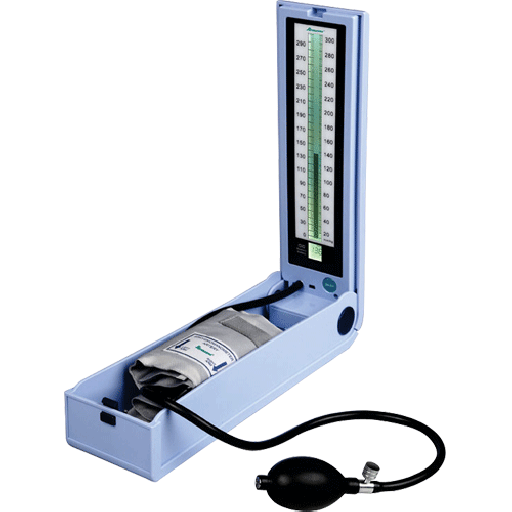
\includegraphics[width=0.45\textwidth,height=\textheight]{images/pngegg.png}
\end{center}

\subsection{Digital BP Monitor}\label{digital-bp-monitor}

\begin{quote}
A digital blood pressure (BP) monitor is an electronic device designed
to measure blood pressure and heart rate. It automates the process of
inflating the cuff, measuring the blood pressure, and displaying the
results, making it easier to use compared to traditional manual
sphygmomanometers.
\end{quote}

\begin{center}
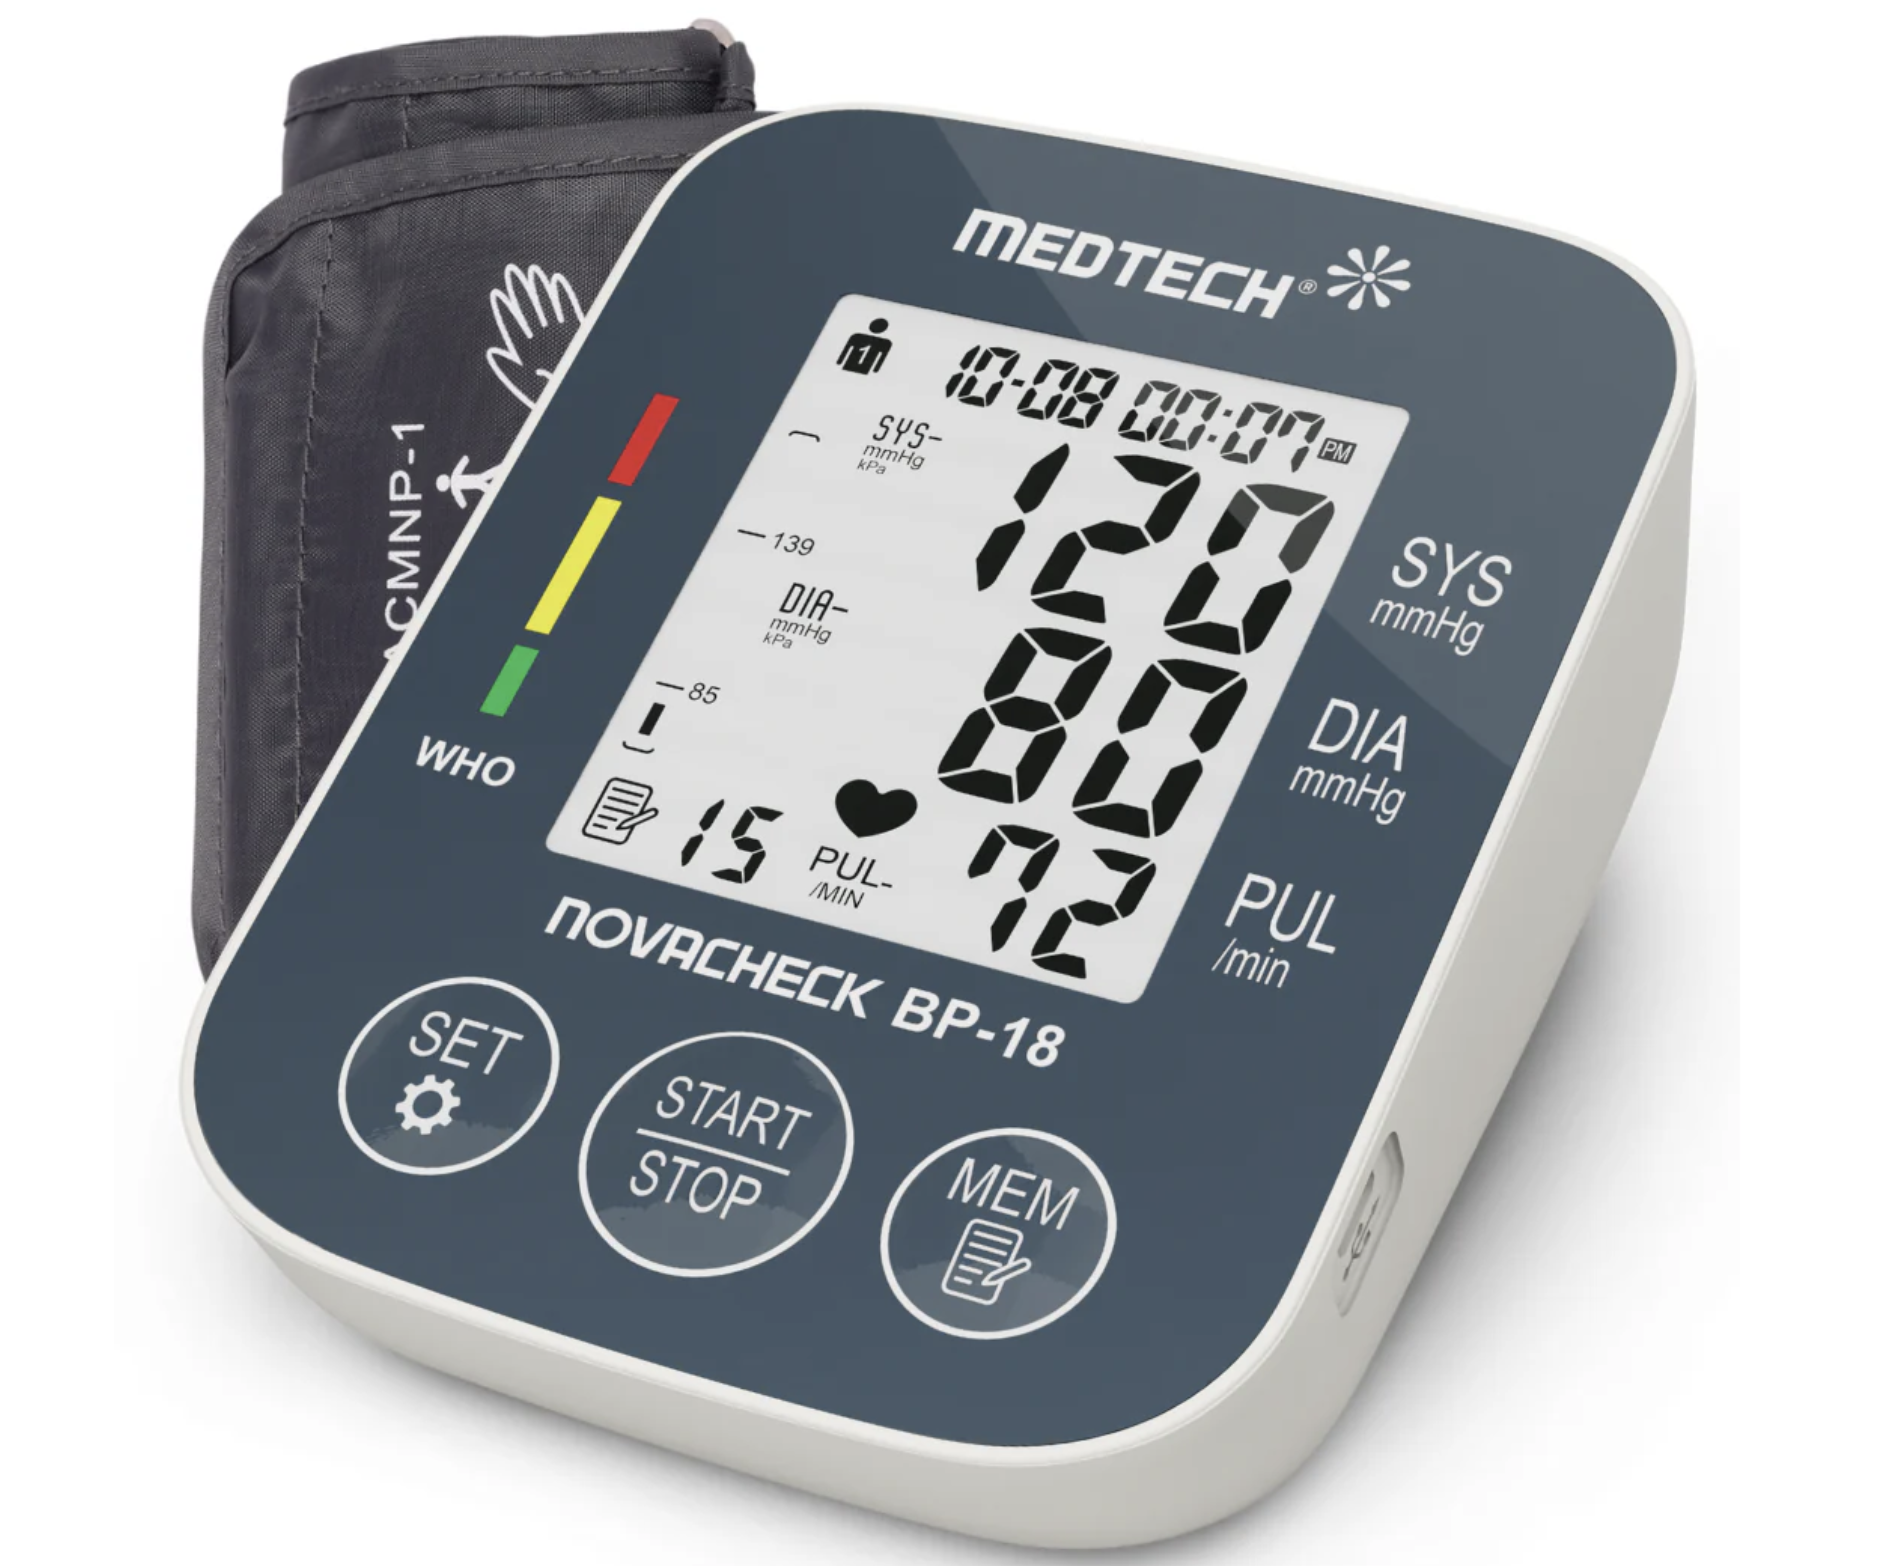
\includegraphics[width=4.5in,height=\textheight]{images/clipboard-3151283748.png}
\end{center}

\section{Procedure}\label{procedure}

\subsection{Sphygmomanometer}\label{sphygmomanometer-1}

\begin{itemize}
\item
  Subject is made to sit parallel to the mercury level of the monitor.
  The mercury knob is made opened.
\item
  Rough side of the cuff is placed on top of the left hand and is tied
  tightly on the brachial artery (point on left hand, where pulse is
  felt).
\item
  Stethoscope is placed on brachial artery just below the cuff's sensor
  to record Korotkoff's sounds (Heard when medical personnel listen for
  when they are taking blood pressure using a non invasive procedure).
\item
  The pressure is increased till 180mmHg using rubber bulb or inflator.
\end{itemize}

\subsubsection{Note}\label{note}

\begin{itemize}
\item
  Onset point of Korotkoff sound is the Systolic pressure
\item
  Dying of the Korotkoff sound is Diastolic pressure
\end{itemize}

\begin{quote}
and the readings are taken accordingly.
\end{quote}

\subsection{Digital Blood Pressure
Monitor}\label{digital-blood-pressure-monitor}

\begin{quote}
Digital sphygmomanometers are automated, providing blood pressure
reading without needing someone to operate the cuff or listen to the
blood flow.
\end{quote}

\section{Observation}\label{observation}

\setlength{\LTpost}{0mm}
\begin{longtable*}{lrrl}
\caption*{
{\large Observation table for Mechanical BP meter} \\ 
{\small Data taken from Mechanical BP meter}
} \\ 
\toprule
Student Name & BP Readings & Mean Arterial Pressure (MAP) & Analysis \\ 
\midrule\addlinespace[2.5pt]
Kulkarni sir & 120/80 & 93.33 & Normal \\ 
Monika & 110/70 & 83.33 & Normal \\ 
Kushaal & 130/90 & 103.33 & Pre-hypertension \\ 
Namyatha & 120/83 & 95.33 & Normal \\ 
Karthik & 125/85 & 98.33 & Pre-hypertension \\ 
Janane & 110/65 & 80.00 & Normal \\ 
Omar & 110/70 & 83.33 & Normal \\ 
Hasan & 100/70 & 80.00 & Normal \\ 
Saad & 120/85 & 96.66 & Normal \\ 
Manasa & 90/86 & 87.33 & Normal \\ 
Mayuri & 110/75 & 86.66 & Normal \\ 
Nidhi & 110/90 & 96.66 & Normal \\ 
Lakshita & 100/70 & 80.00 & Normal \\ 
\bottomrule
\end{longtable*}
\begin{minipage}{\linewidth}
Source: DTE Lab, 4th floor, Dept of Medical Electronics\\
\end{minipage}

\setlength{\LTpost}{0mm}
\begin{longtable*}{lrrl}
\caption*{
{\large Observation table for Digital BP meter} \\ 
{\small Data taken from Digital BP meter}
} \\ 
\toprule
Student Name & BP Readings & Mean Arterial Pressure (MAP) & Analysis \\ 
\midrule\addlinespace[2.5pt]
Kulkarni sir & 117/85 & 95.66 & Normal \\ 
Monika & 99/64 & 75.66 & Hypotension \\ 
Kushaal & 112/80 & 90.66 & Normal \\ 
Namyatha & 126/74 & 91.33 & Normal \\ 
Karthik & 119/80 & 93.00 & Normal \\ 
Janane & 112/70 & 84.00 & Normal \\ 
Omar & 117/67 & 83.66 & Normal \\ 
Hasan & 98/70 & 79.33 & Hypotension \\ 
Saad & 115/76 & 89.00 & Normal \\ 
Manasa & 82/69 & 73.33 & Hypotension \\ 
Mayuri & 115/76 & 89.00 & Normal \\ 
Nidhi & 100/80 & 86.66 & Normal \\ 
Lakshita & 85/73 & 77.00 & Hypotension \\ 
\bottomrule
\end{longtable*}
\begin{minipage}{\linewidth}
Source: DTE Lab, 4th floor, Dept of Medical Electronics\\
\end{minipage}

\section{Calculations}\label{calculations}

\[
MAP = \frac{1}{3} (SP - DP) + DP
\]

where \(MAP\) is Mean Arterial Pressure

\begin{description}
\item[Sphygmomanometer]
\[
\frac{1}{3} (120 - 80) + 80 = 93.33
\]
\item[Digital BP meter]
\[
\frac{1}{3} (117 - 85) + 85 = 95.66
\]
\end{description}

\section{Analysis}\label{analysis}

\begin{itemize}
\item
  We observe that there is a change in \texttt{MAP} with change in BP
  levels.
\item
  Generally, if there's a difference between systolic and diastolic
  pressure is \texttt{40\ mmHg}, the subject is considered to be normal.
\item
  If the difference between systolic and diastolic pressure ranges
  between \texttt{30\ -\ 50\ mmHg}, the subject is considered to be
  \texttt{normal} depending on the conditions.
\item
  If systolic and diastolic pressure difference is \(<30mmHg\), the
  subject has low BP which leads to hypotension.
\item
  If difference is \(>50mmHg\), the subject has high BP which leads to
  hypertension.
\end{itemize}

\section{Result}\label{result}

\begin{quote}
The working and analysis of mechanical and electronic BP meters are
analyzed.
\end{quote}

\bookmarksetup{startatroot}

\chapter{Electrocardiogram (ECG)
Measurement}\label{electrocardiogram-ecg-measurement}

\section{Aim}\label{aim-1}

\begin{quote}
Aquisition of ECG signal with the help of Power lab and Bio-pac systems.
\end{quote}

\section{Theory}\label{theory-1}

\begin{quote}
Electrocardiogram records from the body surface and registers the
differences in electrical potential generated by the heart. Signal
recorded is determined by action potentials generated by millions of
individual cells and their sequence of activation. A multitude of
factors (both cardiac and extracardiac) alter the final electrical
signal. For instance, the electrical forces generated by heart are
subsequently altered by the position of the heart within the body, the
nature of intervening tissue and the distance to the recording
electrode.
\end{quote}

\begin{itemize}
\item
  Lead 1 = RA, LA, RL
\item
  Lead 2 = RA, LL, RL
\item
  Lead 3 = LA, LL, RL
\end{itemize}

\begin{center}
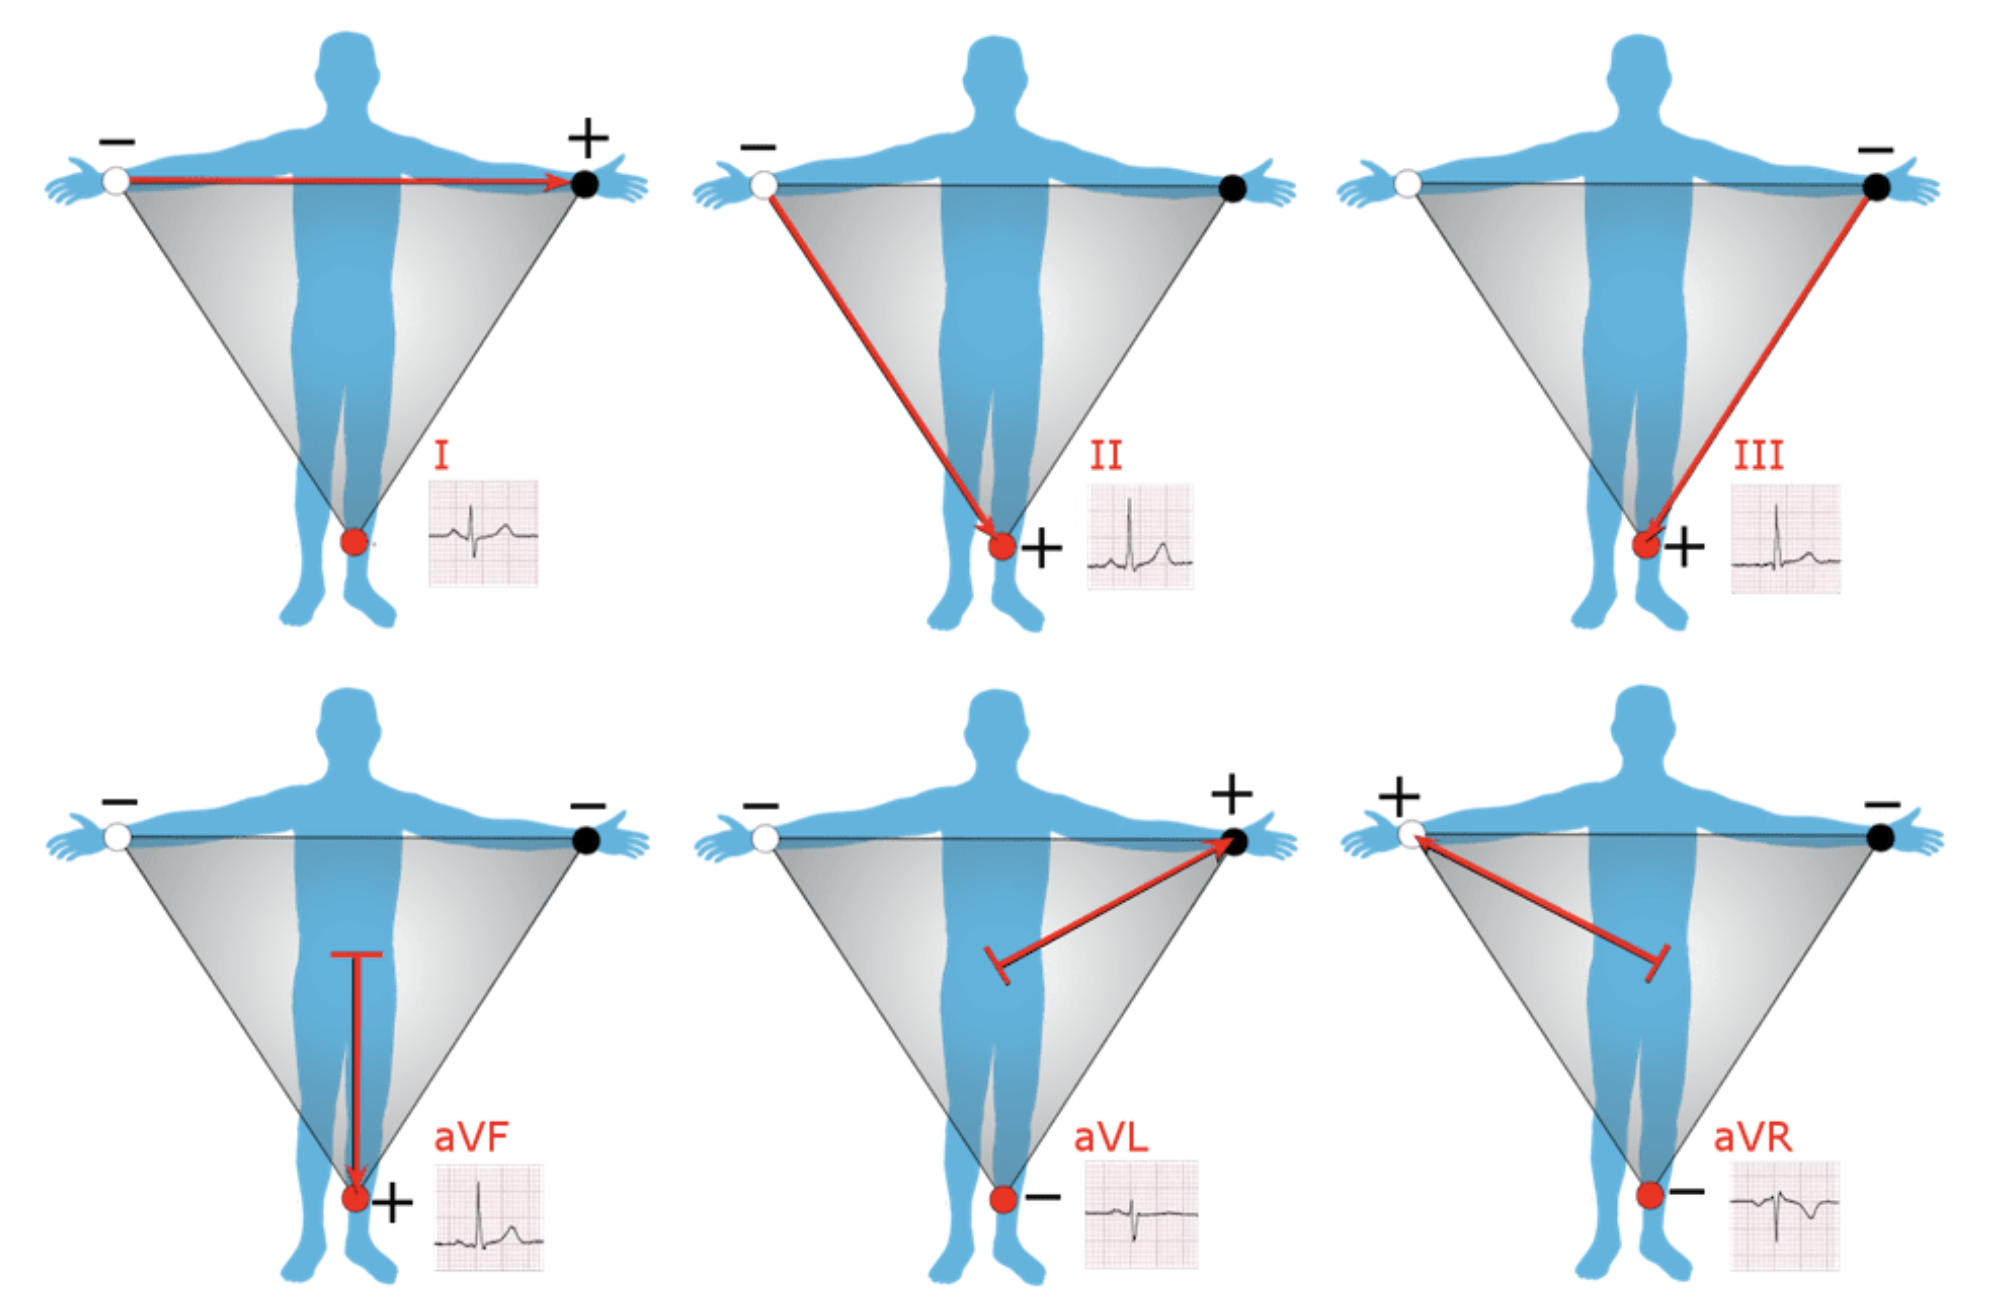
\includegraphics[width=5.82292in,height=\textheight]{images/clipboard-2797361598.png}
\end{center}

\begin{center}
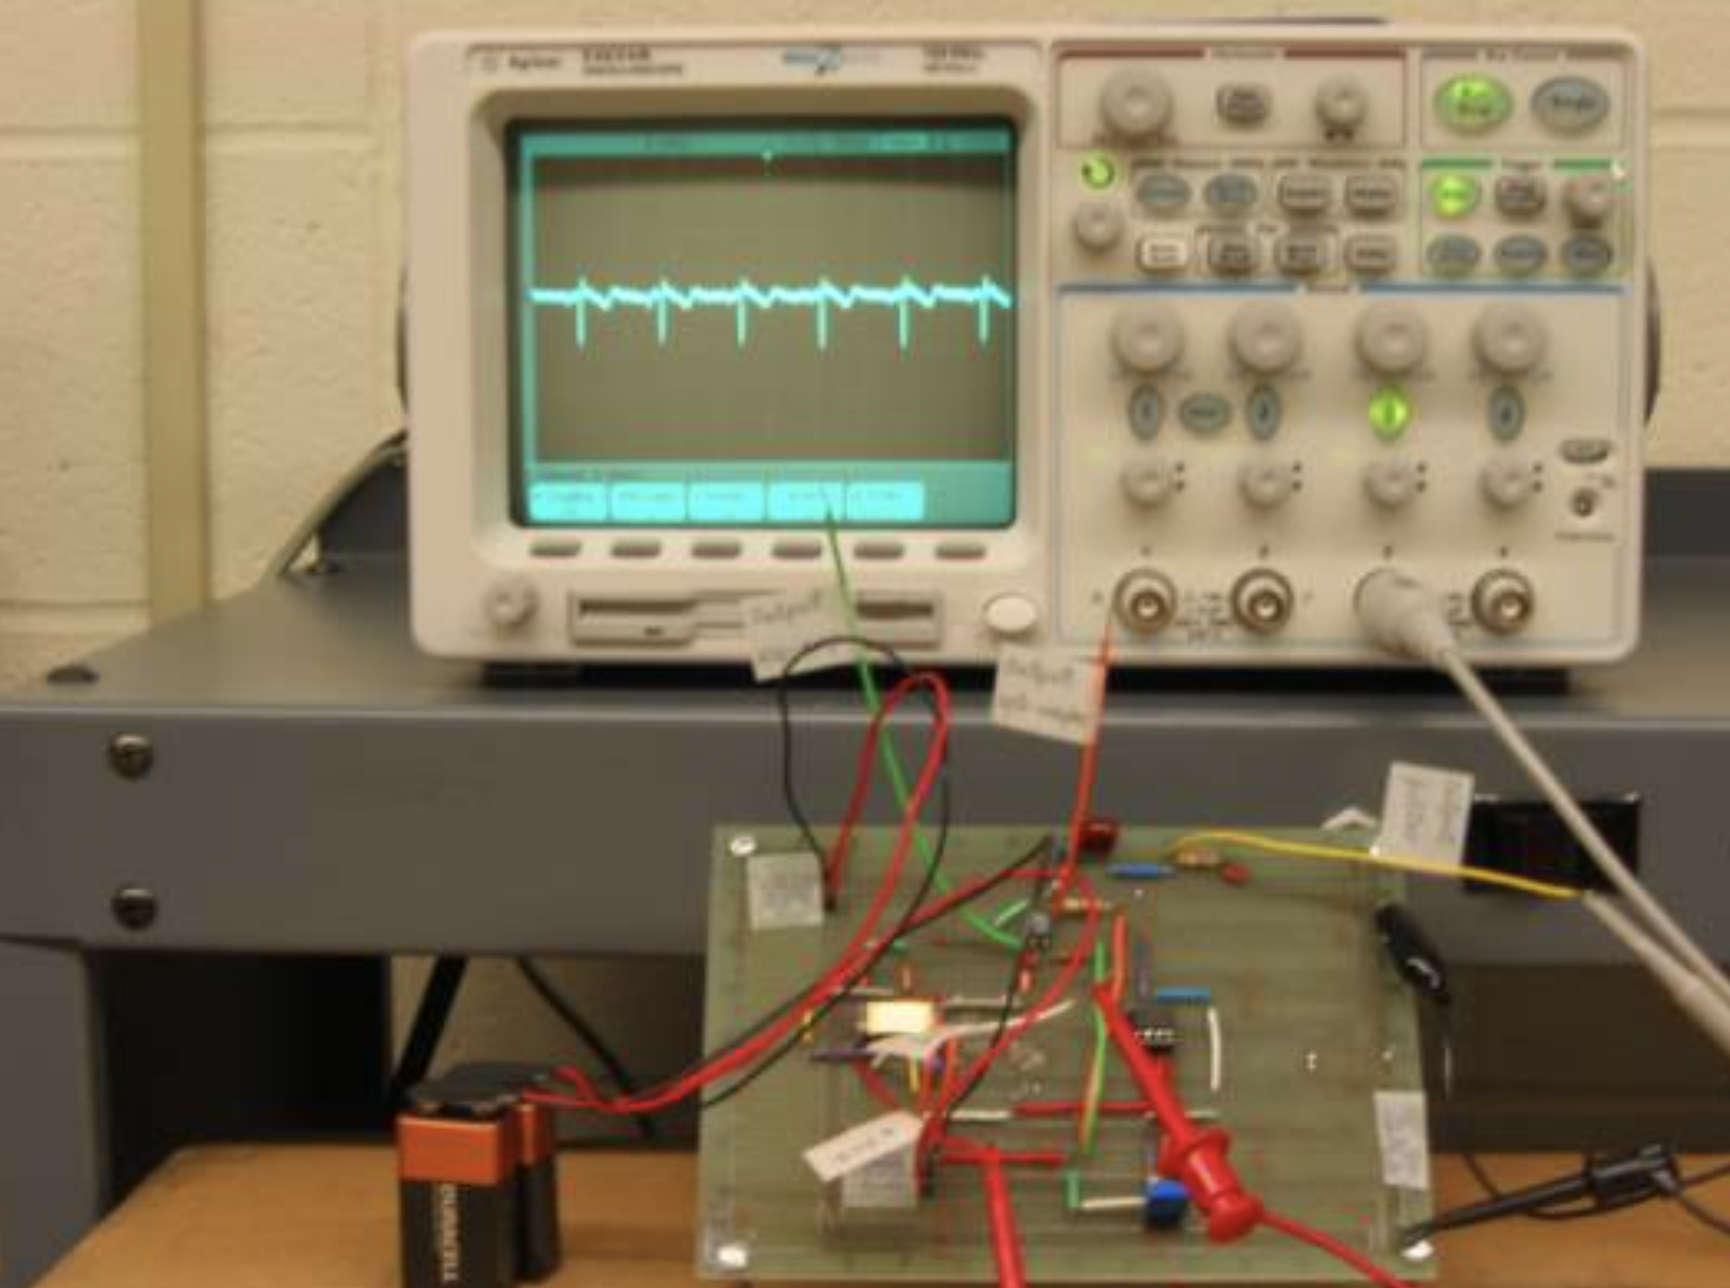
\includegraphics[width=0.48\textwidth,height=\textheight]{images/clipboard-91339677.png}
\end{center}

\begin{center}
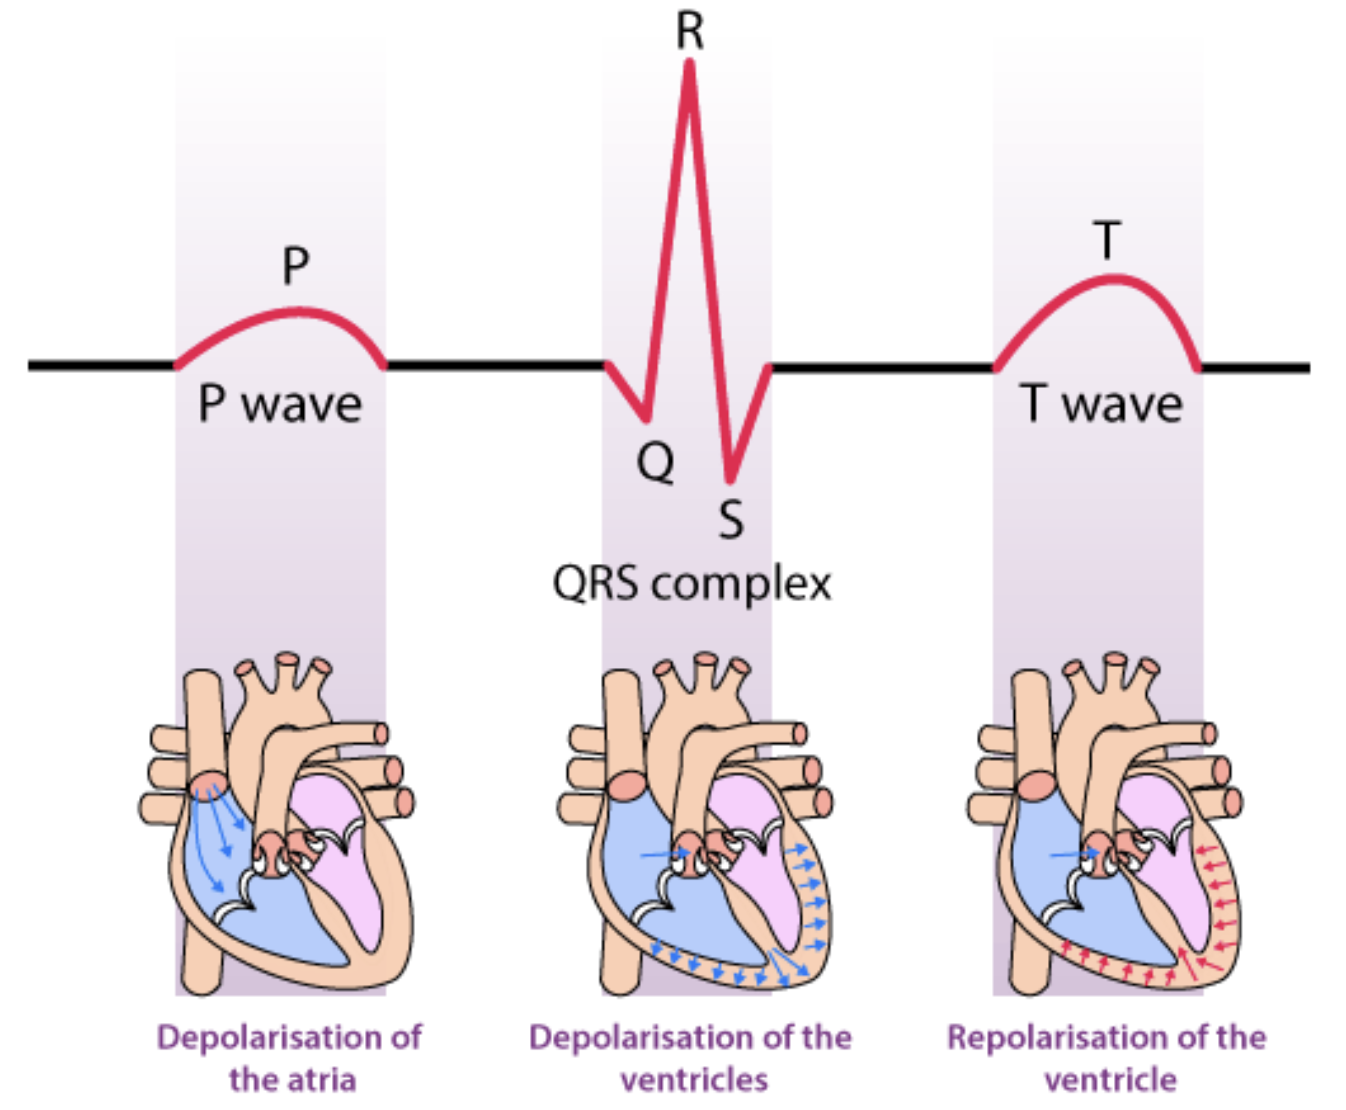
\includegraphics[width=0.51\textwidth,height=\textheight]{images/clipboard-1351516102.png}
\end{center}

\subsection{Bio-pac system}\label{bio-pac-system}

We aquire ECG signal using the Bio-pac system

\begin{center}
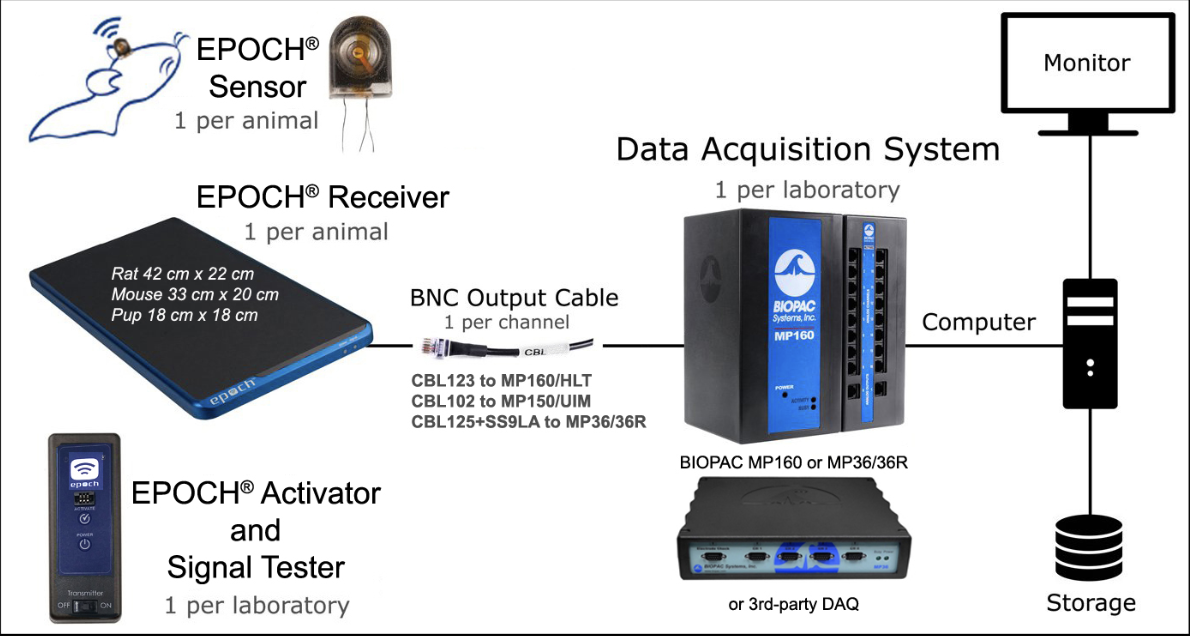
\includegraphics[width=0.74\textwidth,height=\textheight]{images/clipboard-1355974490.png}
\end{center}

\section{Procedure}\label{procedure-1}

\begin{enumerate}
\def\labelenumi{\arabic{enumi}.}
\tightlist
\item
  BIOPAC lessons are opened on the PC
\item
  Select \texttt{ECG1} and click OK.
\item
  Electrodes are placed on respective channel (CH:2) according to lead
  configurations. Transducer used is SS2L and subject should be at rest.
\item
  System is first calibrated and checked for proper contact of
  electrodes.
\item
  ECG setup is thus simulated, and the readings are recorded for each
  lead configuration
\item
  After recording the signals, BIOPAC lessons is clicked to save
  readings, which display the peak to peak voltage.
\item
  L1 + L3 = L2 is thus verified.
\end{enumerate}

\section{Observation}\label{observation-1}

\begin{longtable*}{lrrrr}
\caption*{
{\large ECG Lead analysis} \\ 
{\small Peak-to-Peak Values, Frequencies, Time Intervals, and Beats per Minute (BPM) for ECG Leads}
} \\ 
\toprule
Lead Number & Peak to Peak & Frequency f (in Hz) & Time (in sec) = 1/f & Beats per Min = 60/T \\ 
\midrule\addlinespace[2.5pt]
Lead 1 & 0.47 & 1.27 & 0.78 & 76.92 \\ 
Lead 2 & 0.55 & 1.25 & 0.80 & 75.00 \\ 
Lead 3 & 0.08 & 1.26 & 0.79 & 75.94 \\ 
\bottomrule
\end{longtable*}

\section{Analysis}\label{analysis-1}

The Biopac software shows consistent heart rate readings across all
leads (75-77 bpm) indicating accurate and stable heart rate rhythm
detection.

ECG analysis if the subject is acquired and Lead1 + lead3 = Lead2 was
verified. Using frequency of the signal acquired, the bpm was also
found.

Lead 1 = 0.47

Lead 3 = 0.08

Lead 2 = 0.47 + 0.08 = 0.55

\(\frac{1}{f} = T = 0.78\) and \(\frac{60}{0.78} = 76.92\)

\section{Result}\label{result-1}

The ECG signal was aquired and L1 + L3 = L2 is verified.

\bookmarksetup{startatroot}

\chapter{Electromyogram (EMG)
Measurement}\label{electromyogram-emg-measurement}

\section{Aim}\label{aim-2}

\begin{quote}
Acquisition of EMG Signal with the help of nerve stimulation and
Bio-pack Systems.
\end{quote}

\section{Apparatus}\label{apparatus-1}

\begin{itemize}
\item
  EMG Stimulator
\item
  Ring electrodes and other hardware components
\item
  Biopac software
\end{itemize}

\section{Theory}\label{theory-2}

\begin{quote}
Electromyography records electrical activity produced by skeletal
muscles. The signal is determined by action potentials generated by
muscle fibers during contraction and relaxation. EMG signals provide
valuable information to diagnose neuromuscular disorders and study motor
control. EMG results can reveal nerve dysfunction, muscle dysfunction or
problems with nerve-to-muscle signal transmission. Motor neurons
transmit electrical signals that cause muscles to contract. An EMG uses
tiny devices called electrodes to translate these signals into graphs,
sounds or numerical values that are then interpreted by a specialist.
\end{quote}

\section{Nerve stimulator}\label{nerve-stimulator}

\begin{itemize}
\tightlist
\item
  The selector has two options, the EMG, and the stimulator. The EMG is
  used to record the EMG signal and the stimulator is used to generate
  stimulus in the body to obtain a signal.
\item
  To produce a stimulus, the stimulator is set to 100ms and the
  intensity is varied accordingly.
\item
  After selecting EMG in the selector region, the gain is set to 1 and
  is set on the EMG mode to enable the acquisition of the signal.
\item
  Two wires from this system are connected as input to the Ag/AgCl
  electrodes placed on the fingers.
\item
  Two wires are connected as output to the storage oscilloscope to
  record the EMG signal.
\end{itemize}

\begin{center}
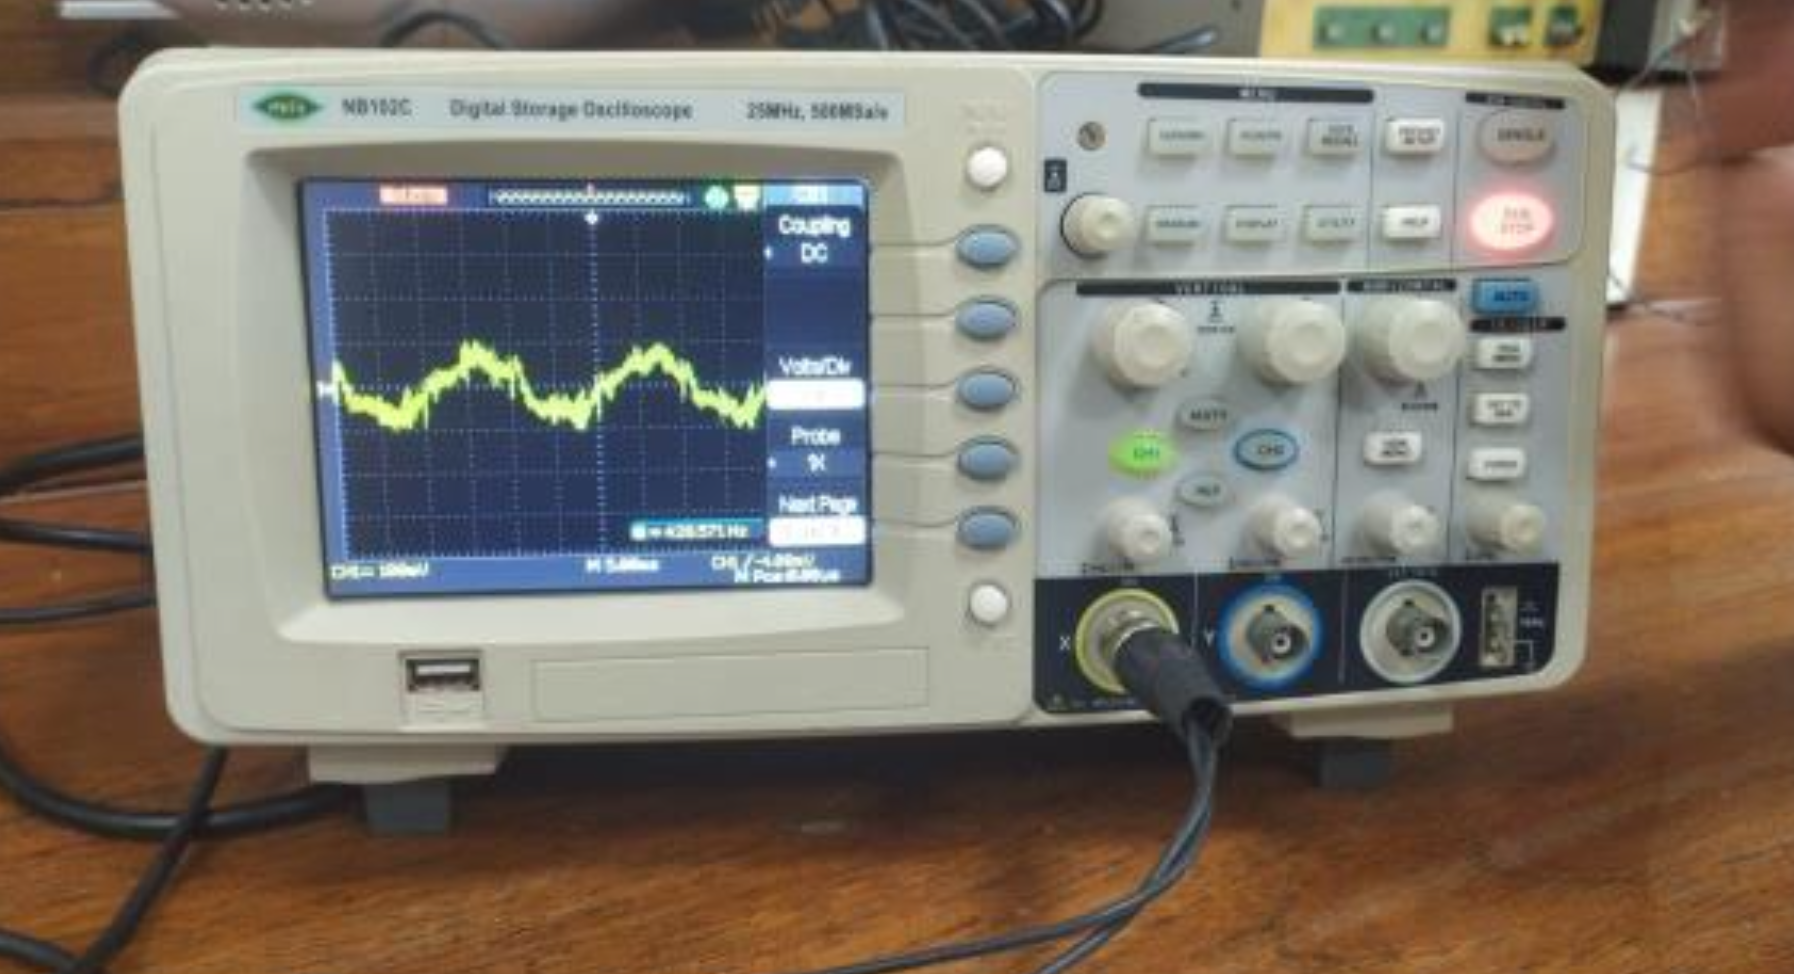
\includegraphics[width=4.8125in,height=\textheight]{images/clipboard-2396942276.png}
\end{center}

\subsection{Procedure}\label{procedure-2}

\begin{enumerate}
\def\labelenumi{\arabic{enumi}.}
\tightlist
\item
  The Ag/AgCl electrodes are placed on the index finger (+ve), ring
  finger (-ve) of the right hand and the reference electrode is placed
  on any finger on the left hand.
\item
  The subject should not be wearing any metallic accessories on the hand
  since it creates noise while acquiring the signal.
\item
  The fingers of both the hands are then contracted and relaxed until a
  spike is observed on the oscilloscope.
\item
  The amplitude of the signal is calculated and then multiplied with 100
  mV and the amplitude of the EMG signal is thus obtained.
\end{enumerate}

\begin{center}
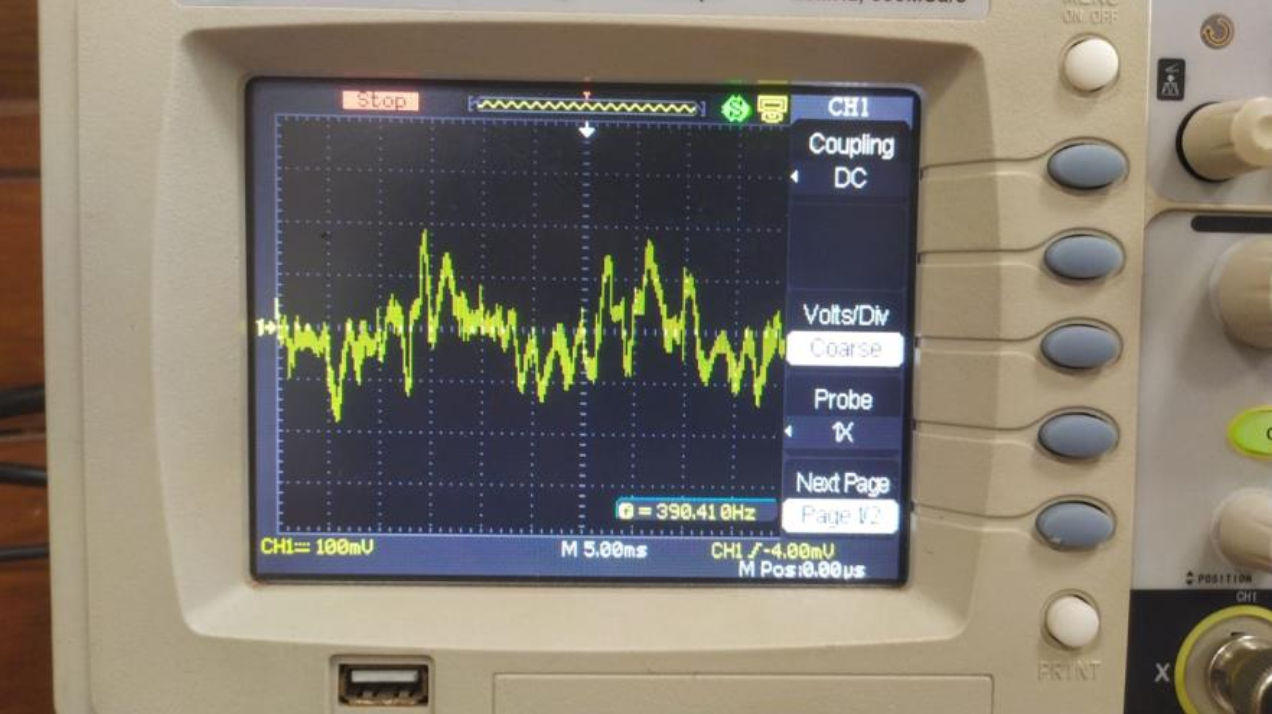
\includegraphics[width=4.77083in,height=\textheight]{images/clipboard-1109147105.png}
\end{center}

\section{Bio-PAC system}\label{bio-pac-system-1}

Using the Bio-pack system, we acquire the EMG signal.

\subsection{Procedure}\label{procedure-3}

\begin{enumerate}
\def\labelenumi{\arabic{enumi}.}
\tightlist
\item
  Select icon BSL Lessons.
\item
  Select EMG 1. Click Ok.
\item
  Colour code is mentioned to connect the electrodes.
\item
  Click Calibrate. The subject is asked to clench fist as hard as
  possible and then release.
\item
  The subject also uses headphones to listen to the noise.
\item
  Statistical parameters are measured and recorded.
\item
  Minimum, maximum, peak-to-peak, mean, standard deviation is found and
  are plotted and recorded.
\end{enumerate}

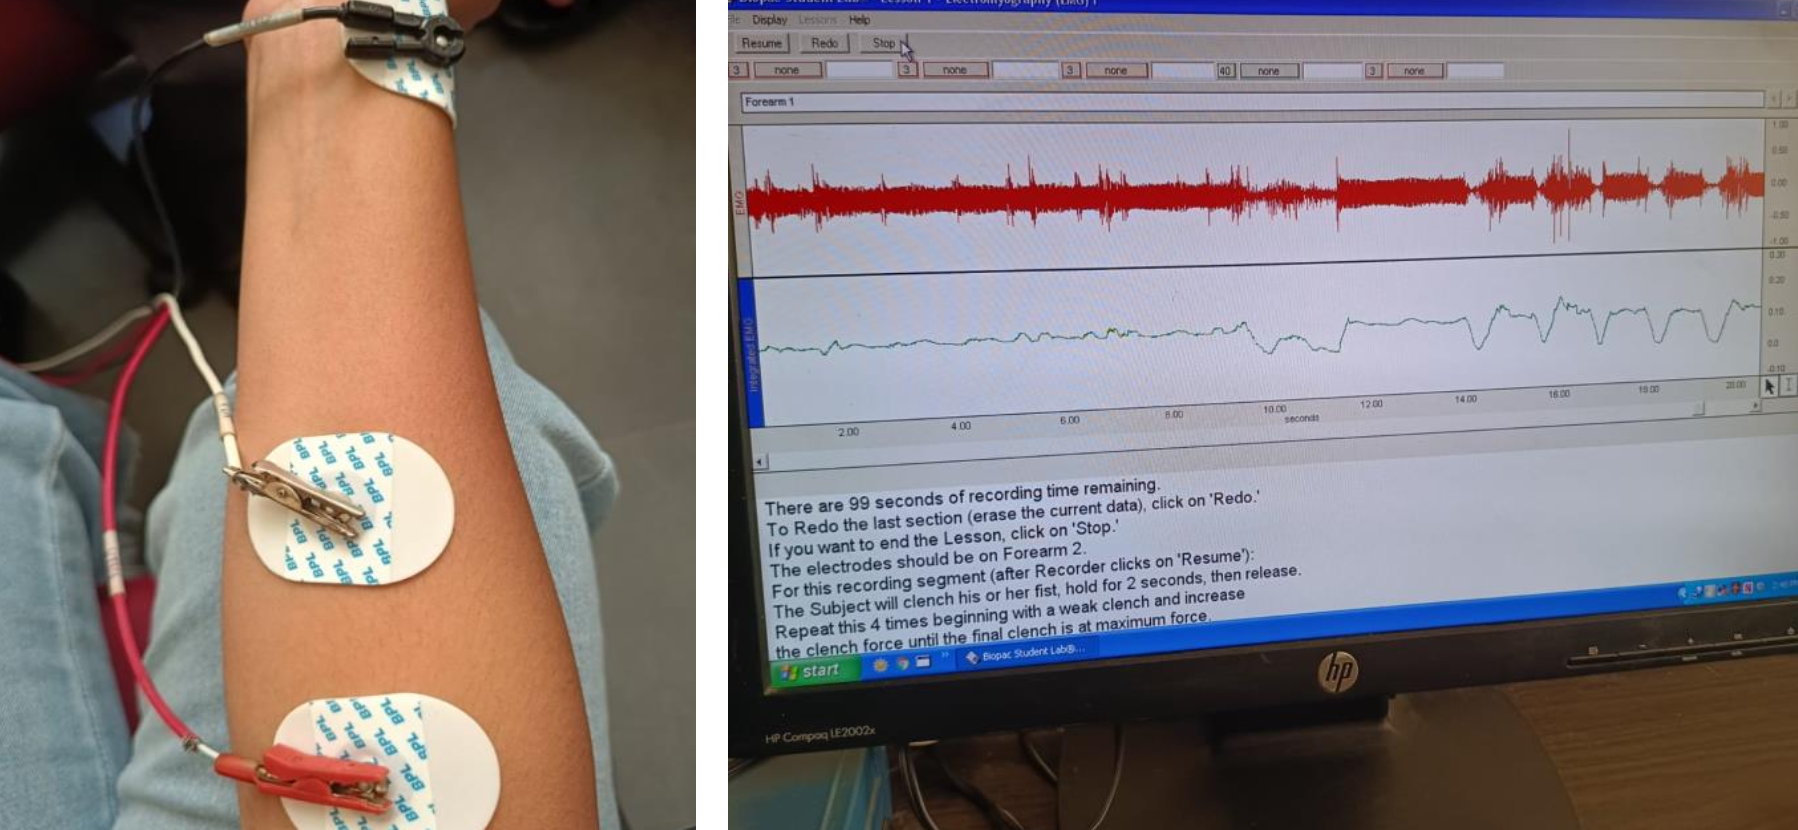
\includegraphics[width=6.46875in,height=\textheight]{images/clipboard-1236183346.png}

\section{Observation}\label{observation-2}

\subsection{Nerve stimulator}\label{nerve-stimulator-1}

\begin{longtable*}{lr}
\caption*{
{\large EMG} \\ 
{\small Muscle contraction voltages for each subject}
} \\ 
\toprule
Subject & Muscle contraction voltage (in Volts) \\ 
\midrule\addlinespace[2.5pt]
Kulkarni sir & 10.0 \\ 
Mayuri & 6.0 \\ 
Namyatha & 7.0 \\ 
Kushaal & 7.1 \\ 
\bottomrule
\end{longtable*}

\subsection{Bio-PAC system}\label{bio-pac-system-2}

\begin{longtable*}{lrrrrr}
\caption*{
{\large EMG Biopac analysis} \\ 
{\small Peak-to-Peak Values, Frequencies, Mean and Std Deviations}
} \\ 
\toprule
Hands of subjects & Peak to Peak voltage (in mV) & Vmax (in mV) & Vfreq (in Hz) & Mean (mV-s) & Std. Dev (in mV) \\ 
\midrule\addlinespace[2.5pt]
Left Hand\_1 & 1.7120 & 0.893 & 0.383 & 0.113 & 0.150 \\ 
Left Hand\_2 & 1.5890 & 0.672 & 1.586 & 0.105 & 0.147 \\ 
Right Hand\_1 & 1.5011 & 0.229 & 0.304 & 0.129 & 0.116 \\ 
Right Hand\_2 & 1.9590 & 0.860 & 0.060 & 0.114 & 0.150 \\ 
\bottomrule
\end{longtable*}

\section{Analysis}\label{analysis-2}

The EMG signals are acquired from the above-mentioned approaches (Ring
electrodes and Surface electrodes) The amplitude of signals for peak
voltage and mean voltages are analyzed to identify various muscle
conditions like Muscle weakness and neuro muscular abnormalities. This
also helps us find out the subjects dominant and non-dominant hand by
assessing the mean voltage of a particular interval.

\% Difference in mean of weakest and strongest clench can be found to
find the dominant hand.

\textbf{Left hand:} \(\frac{0.129 - 0.114}{0.129} * 100 = 11.62\%\)

\textbf{Right hand:} \(\frac{0.113 - 0.105}{0.113} * 100 = 7.079\%\)

Thus, the subject's \textbf{Right hand} is the dominant hand from the
above analysis.

\section{Result}\label{result-2}

The EMG signal is thus acquired and recorded.

\bookmarksetup{startatroot}

\chapter{EEG Signal Acquisition with Bio-PAC and
ENOBIO}\label{eeg-signal-acquisition-with-bio-pac-and-enobio}

\section{Aim}\label{aim-3}

\begin{quote}
Acquisition of EEG Signal using Bio-PAC using Bio-PAC system.
\end{quote}

\section{Theory}\label{theory-3}

\subsection{EEG Electrode Placement}\label{eeg-electrode-placement}

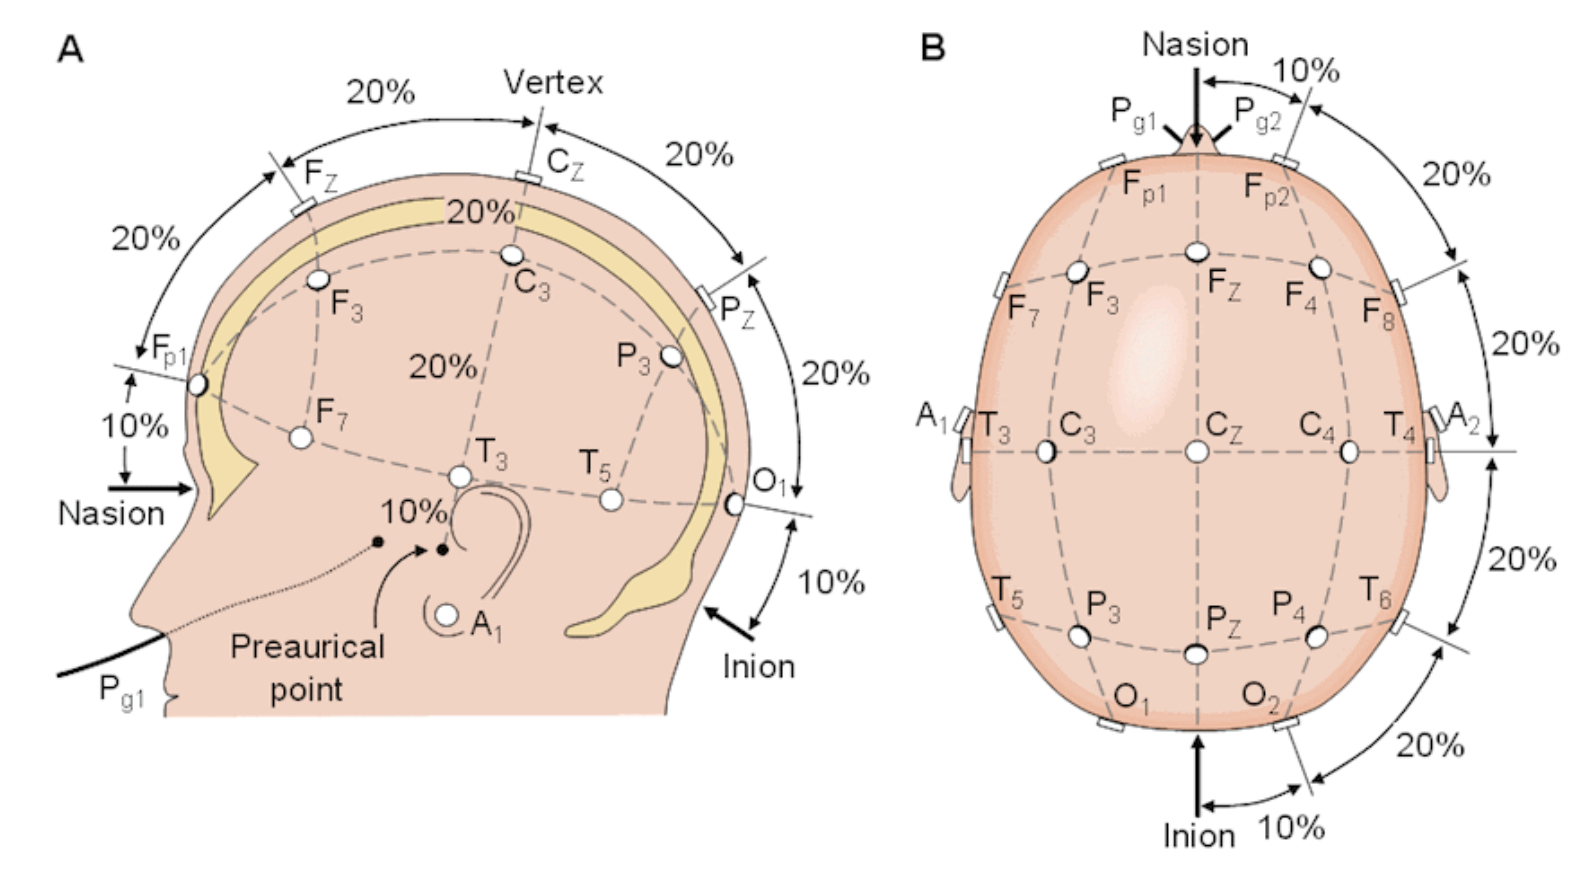
\includegraphics[width=5.63542in,height=\textheight]{images/clipboard-1080795871.png}

\begin{itemize}
\tightlist
\item
  Electrodes are typically placed on the scalp according to the
  International 10-20 system, which standardizes positions based on the
  relative distances between key points on the head.
\item
  Each electrode location is labeled with a combination of a letter and
  a number (e.g., F3, P4), where the letter indicates the brain region
  (e.g., F for frontal, P for parietal) and the number indicates the
  hemisphere and position.
\end{itemize}

\subsection{Frequency bands of EEG}\label{frequency-bands-of-eeg}

\begin{itemize}
\tightlist
\item
  Delta - \(\delta\) (0.5-4 Hz): Associated with deep sleep.
\item
  Theta - \(\theta\) (4-8 Hz): Related to light sleep, relaxation, and
  drowsiness.
\item
  Alpha - \(\alpha\) (8-13 Hz): Linked to relaxed wakefulness, often
  seen when eyes are closed.
\item
  Beta - \(\beta\) (13-30 Hz): Associated with active thinking, focus,
  and problem-solving.
\item
  Gamma - \(\gamma\) (30-100 Hz): Related to high-level information
  processing and cognitive functioning.
\end{itemize}

\section{Using Bio-PAC}\label{using-bio-pac}

\subsection{Procedure for Bio-PAC}\label{procedure-for-bio-pac}

\begin{enumerate}
\def\labelenumi{\arabic{enumi}.}
\tightlist
\item
\end{enumerate}

\begin{itemize}
\tightlist
\item
  Active Electrode (A1) {[}Red wire{]}: Place this electrode on the
  Forehead Right.
\item
  Reference Electrode (R) {[}Black wire{]}: Place this electrode on the
  mastoid bone behind the ear or on an earlobe.
\item
  Ground Electrode (G) {[}White wire{]}: Place this electrode on the
  Forehead Left.
\end{itemize}

\begin{enumerate}
\def\labelenumi{\arabic{enumi}.}
\setcounter{enumi}{1}
\item
  To ensure calibration of electrodes, go to \texttt{Bio-PAC}
  \textgreater{} \texttt{Lesson3} \textgreater{} \texttt{channel\ 1} and
  select \texttt{EEG1}. Specify the channels associated with electrodes
  then click on \texttt{calibrate}.
\item
  Now position the subject away from computer, ask to close their eyes
  and relax. Then carry out recording and saving for each subject
  acquisition data then copy and paste in excel.
\end{enumerate}

\subsection{Observation}\label{observation-3}

\begin{longtable*}{lrrrrrrr}
\caption*{
{\large EEG analysis} \\ 
{\small Statistical analysis of EEG Data from different subjects}
} \\ 
\toprule
Subject ID & Peak to Peak (in micro volts) & Delta & Delta T & Frequency f (in Hz) & Mean & Std. Dev & Samples \\ 
\midrule\addlinespace[2.5pt]
Subject 1 & 19.30228 & 1.0947 & 28.505 & 0.037729 & NA & NA & 8975 \\ 
Subject 2 & 25.17906 & -47.7230 & 24.745 & 0.040400 & 10.11118 & 5.62537 & 8761 \\ 
\bottomrule
\end{longtable*}

\section{Using ENOBIO}\label{using-enobio}

\subsection{Procedure for ENOBIO}\label{procedure-for-enobio}

\begin{enumerate}
\def\labelenumi{\arabic{enumi}.}
\tightlist
\item
  Open the NIC 2 application
\item
  Select appropriate protocol or create one. Drag and drop the channel
  names into the right side bar.
\item
  Ensure all the electrodes are properly touching the skull
\item
  Calibrate and start recording. Use \texttt{.easy} file for analysis in
  Python.
\end{enumerate}

\subsection{Observation}\label{observation-4}

\begin{Shaded}
\begin{Highlighting}[]
\ImportTok{import}\NormalTok{ pandas }\ImportTok{as}\NormalTok{ pd}
\ImportTok{import}\NormalTok{ matplotlib.pyplot }\ImportTok{as}\NormalTok{ plt}
\ImportTok{import}\NormalTok{ seaborn }\ImportTok{as}\NormalTok{ sns}

\CommentTok{\# Read and preprocess the .easy file}
\NormalTok{file\_path }\OperatorTok{=} \StringTok{\textquotesingle{}/Users/karthik/Desktop/Raw EEG Analysis/20240702153206\_JEEVAN 1\_Protocol 1.easy\textquotesingle{}}
\NormalTok{column\_names }\OperatorTok{=}\NormalTok{ [}\SpecialStringTok{f\textquotesingle{}Channel\_}\SpecialCharTok{\{}\NormalTok{i}\OperatorTok{+}\DecValTok{1}\SpecialCharTok{\}}\SpecialStringTok{\textquotesingle{}} \ControlFlowTok{for}\NormalTok{ i }\KeywordTok{in} \BuiltInTok{range}\NormalTok{(}\DecValTok{8}\NormalTok{)] }\OperatorTok{+}\NormalTok{ [}\StringTok{\textquotesingle{}Unused\_1\textquotesingle{}}\NormalTok{, }
\StringTok{\textquotesingle{}Unused\_2\textquotesingle{}}\NormalTok{, }\StringTok{\textquotesingle{}Unused\_3\textquotesingle{}}\NormalTok{, }\StringTok{\textquotesingle{}Unused\_4\textquotesingle{}}\NormalTok{, }\StringTok{\textquotesingle{}Timestamp\textquotesingle{}}\NormalTok{]}

\NormalTok{eeg\_data }\OperatorTok{=}\NormalTok{ pd.read\_csv(file\_path, delim\_whitespace}\OperatorTok{=}\VariableTok{True}\NormalTok{, header}\OperatorTok{=}\VariableTok{None}\NormalTok{, }
\NormalTok{names}\OperatorTok{=}\NormalTok{column\_names)}

\CommentTok{\# Extract only the EEG channels and the timestamp}
\NormalTok{eeg\_channels }\OperatorTok{=}\NormalTok{ eeg\_data[column\_names[:}\DecValTok{8}\NormalTok{]]}
\NormalTok{timestamps }\OperatorTok{=}\NormalTok{ eeg\_data[}\StringTok{\textquotesingle{}Timestamp\textquotesingle{}}\NormalTok{]}

\CommentTok{\# Normalize the data}
\NormalTok{eeg\_channels\_normalized }\OperatorTok{=}\NormalTok{ (eeg\_channels }\OperatorTok{{-}}\NormalTok{ eeg\_channels.mean()) }\OperatorTok{/}\NormalTok{ eeg\_channels.std()}

\NormalTok{plt.figure(figsize}\OperatorTok{=}\NormalTok{(}\DecValTok{18}\NormalTok{, }\DecValTok{12}\NormalTok{))}
\ControlFlowTok{for}\NormalTok{ i, channel }\KeywordTok{in} \BuiltInTok{enumerate}\NormalTok{(eeg\_channels\_normalized.columns):}
\NormalTok{    plt.subplot(}\DecValTok{8}\NormalTok{, }\DecValTok{1}\NormalTok{, i }\OperatorTok{+} \DecValTok{1}\NormalTok{)}
\NormalTok{    sns.lineplot(x}\OperatorTok{=}\NormalTok{timestamps, y}\OperatorTok{=}\NormalTok{eeg\_channels\_normalized[channel])}
\NormalTok{    plt.title(channel)}
\NormalTok{    plt.xlabel(}\StringTok{\textquotesingle{}Timestamp\textquotesingle{}}\NormalTok{)}
\NormalTok{    plt.ylabel(}\StringTok{\textquotesingle{}Normalized Amplitude\textquotesingle{}}\NormalTok{)}

\NormalTok{plt.tight\_layout()}
\NormalTok{plt.show()}
\end{Highlighting}
\end{Shaded}

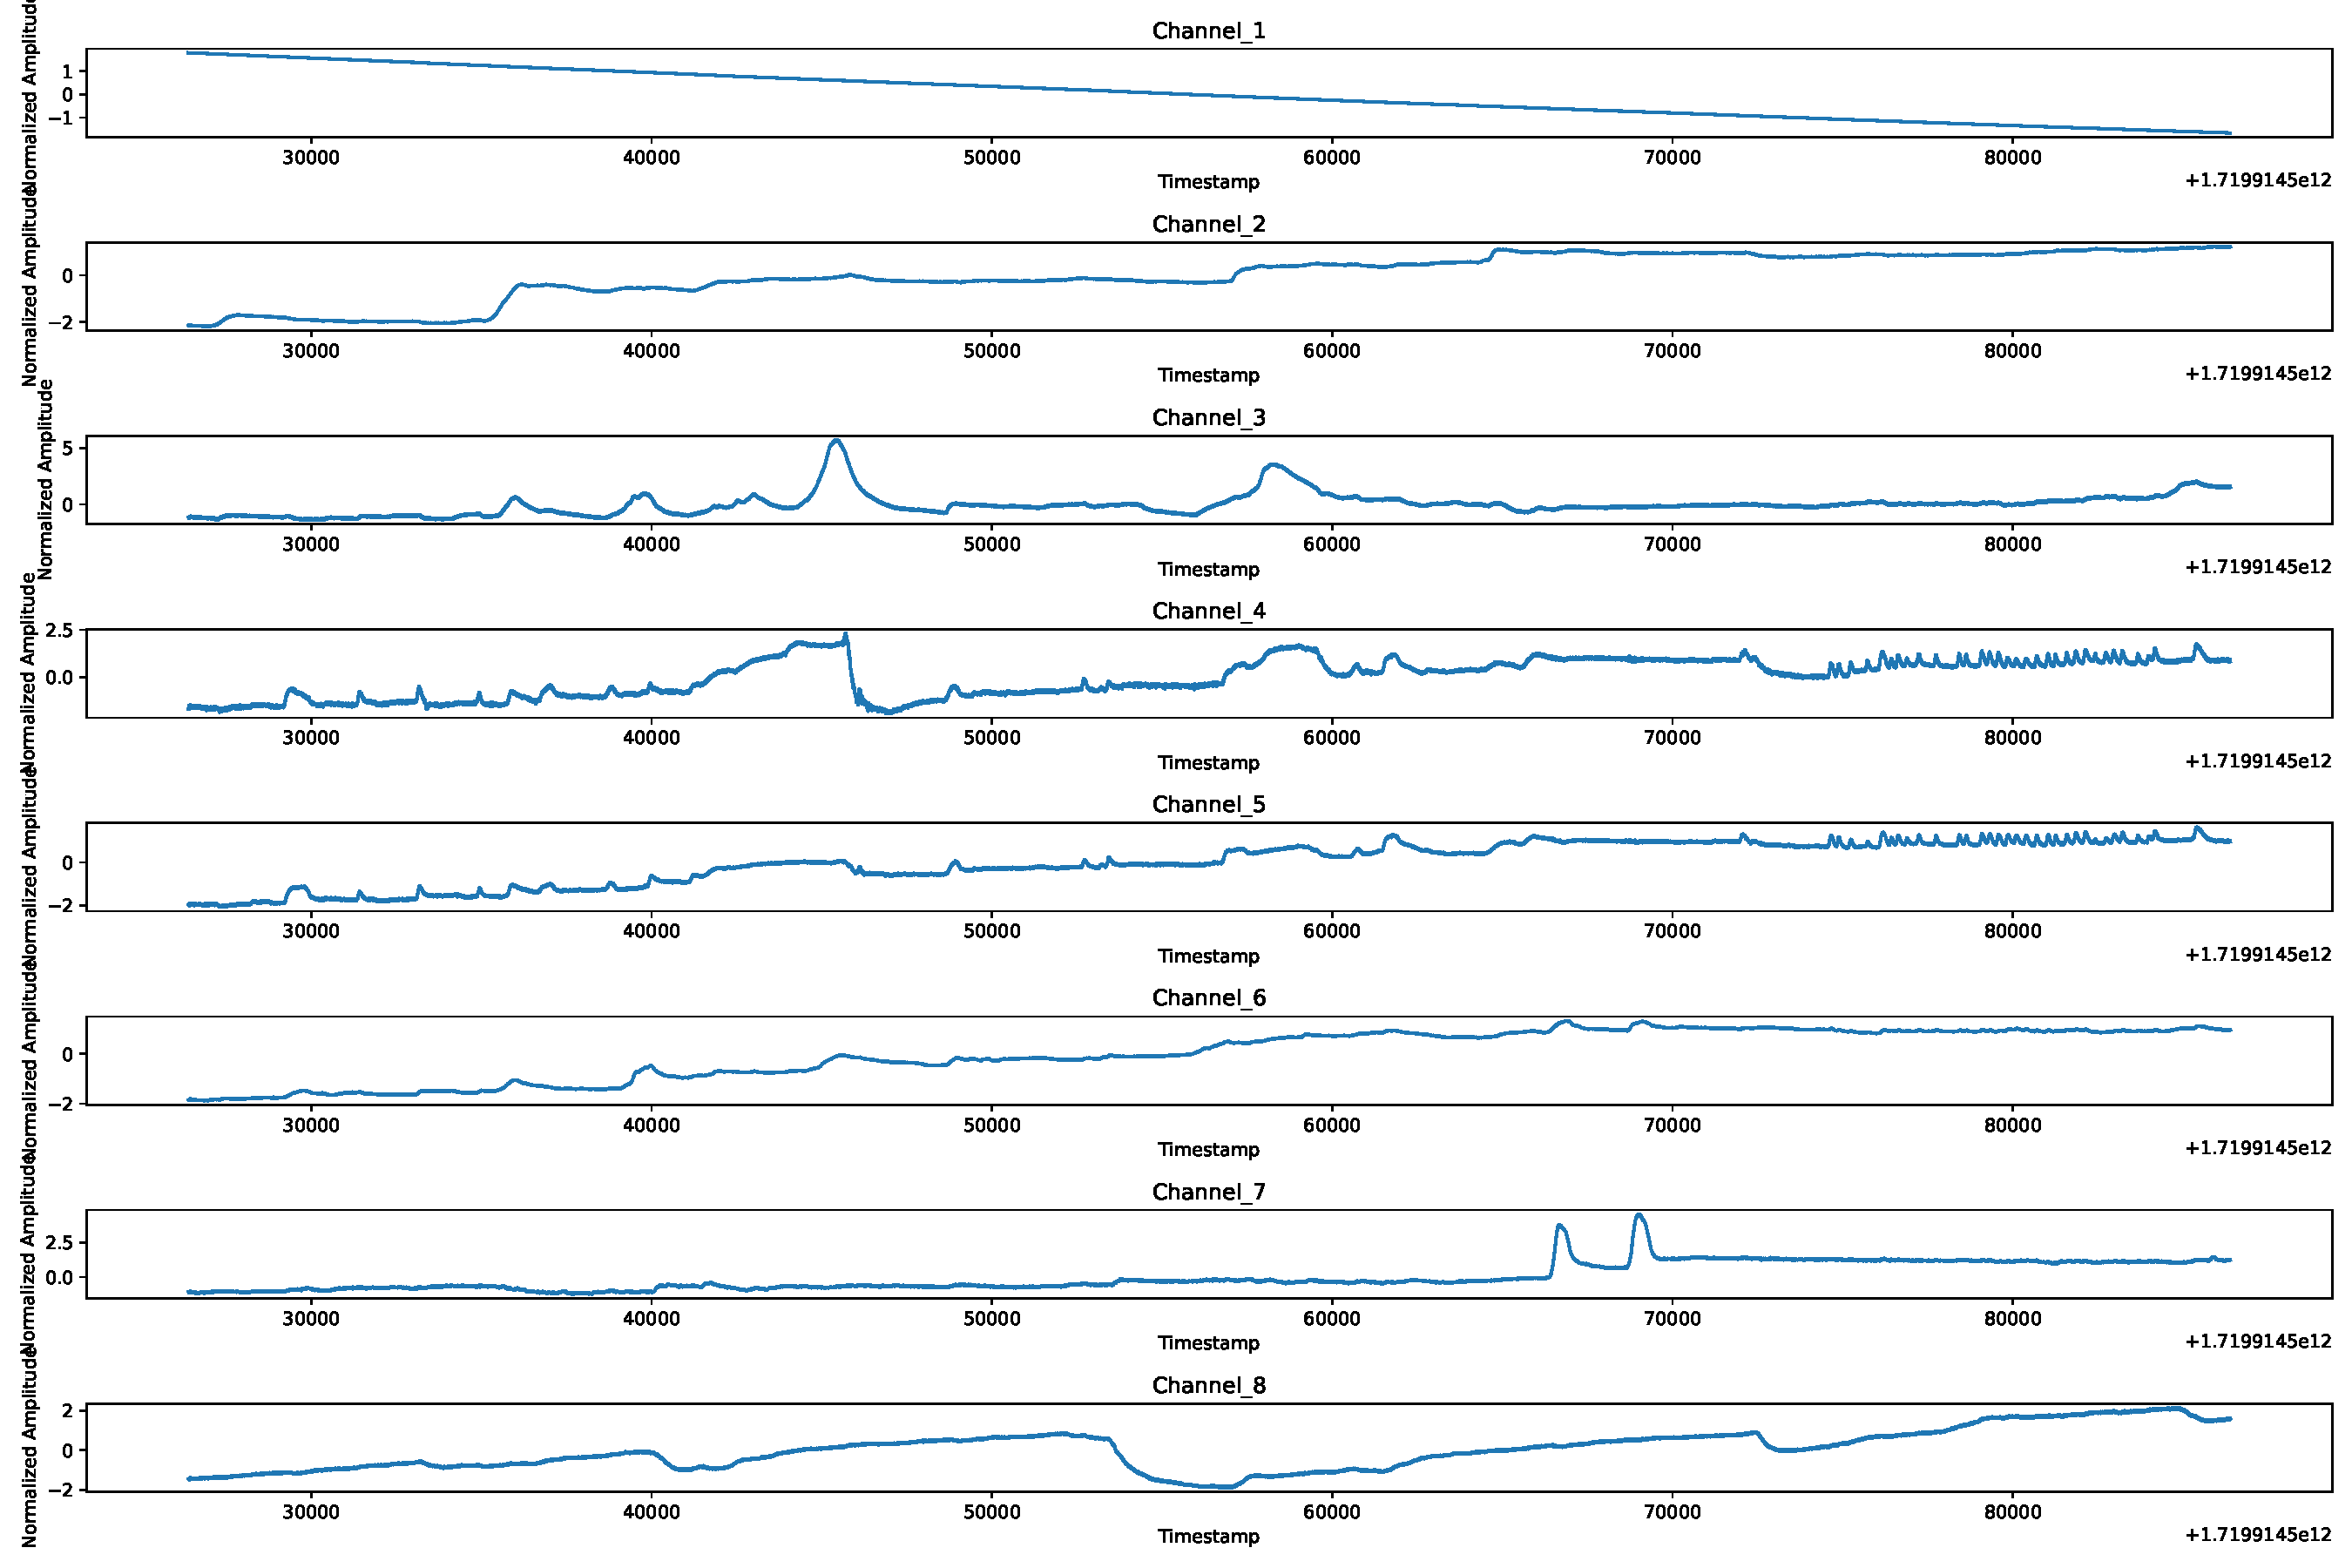
\includegraphics{eeg_files/figure-pdf/unnamed-chunk-2-1.pdf}

Plot for Waveforms of \texttt{channel\_1} to \texttt{channel\_8}

\begin{Shaded}
\begin{Highlighting}[]
\ImportTok{import}\NormalTok{ numpy }\ImportTok{as}\NormalTok{ np}
\ImportTok{from}\NormalTok{ scipy.signal }\ImportTok{import}\NormalTok{ welch}

\NormalTok{statistics }\OperatorTok{=}\NormalTok{ eeg\_channels.describe()}

\BuiltInTok{print}\NormalTok{(}\StringTok{"Basic Statistics for each channel:"}\NormalTok{)}
\end{Highlighting}
\end{Shaded}

\begin{verbatim}
Basic Statistics for each channel:
\end{verbatim}

\begin{Shaded}
\begin{Highlighting}[]
\BuiltInTok{print}\NormalTok{(statistics)}
\end{Highlighting}
\end{Shaded}

\begin{verbatim}
          Channel_1     Channel_2  ...     Channel_7     Channel_8
count  3.000000e+04  3.000000e+04  ...  3.000000e+04  3.000000e+04
mean  -2.090649e+08 -3.681771e+07  ... -3.710497e+07 -2.014704e+07
std    4.776417e+07  2.883546e+06  ...  7.582251e+05  8.920607e+05
min   -2.881841e+08 -4.315196e+07  ... -3.806277e+07 -2.184501e+07
25%   -2.505293e+08 -3.800060e+07  ... -3.766180e+07 -2.088949e+07
50%   -2.106696e+08 -3.701573e+07  ... -3.738470e+07 -2.013874e+07
75%   -1.682614e+08 -3.422193e+07  ... -3.626013e+07 -1.955419e+07
max   -1.233849e+08 -3.321896e+07  ... -3.364406e+07 -1.822300e+07

[8 rows x 8 columns]
\end{verbatim}

\begin{Shaded}
\begin{Highlighting}[]
\CommentTok{\# Plot the power spectral density (PSD) for each channel}
\NormalTok{plt.figure(figsize}\OperatorTok{=}\NormalTok{(}\DecValTok{18}\NormalTok{, }\DecValTok{12}\NormalTok{))}
\ControlFlowTok{for}\NormalTok{ i, channel }\KeywordTok{in} \BuiltInTok{enumerate}\NormalTok{(eeg\_channels.columns):}
\NormalTok{    plt.subplot(}\DecValTok{8}\NormalTok{, }\DecValTok{1}\NormalTok{, i }\OperatorTok{+} \DecValTok{1}\NormalTok{)}
\NormalTok{    freqs, psd }\OperatorTok{=}\NormalTok{ welch(eeg\_channels[channel], fs}\OperatorTok{=}\DecValTok{500}\NormalTok{)}
\NormalTok{    sns.lineplot(x}\OperatorTok{=}\NormalTok{freqs, y}\OperatorTok{=}\NormalTok{psd)}
\NormalTok{    plt.title(}\SpecialStringTok{f\textquotesingle{}PSD {-} }\SpecialCharTok{\{}\NormalTok{channel}\SpecialCharTok{\}}\SpecialStringTok{\textquotesingle{}}\NormalTok{)}
\NormalTok{    plt.xlabel(}\StringTok{\textquotesingle{}Frequency (Hz)\textquotesingle{}}\NormalTok{)}
\NormalTok{    plt.ylabel(}\StringTok{\textquotesingle{}Power/Frequency (dB/Hz)\textquotesingle{}}\NormalTok{)}

\NormalTok{plt.tight\_layout()}
\NormalTok{plt.show()}
\end{Highlighting}
\end{Shaded}

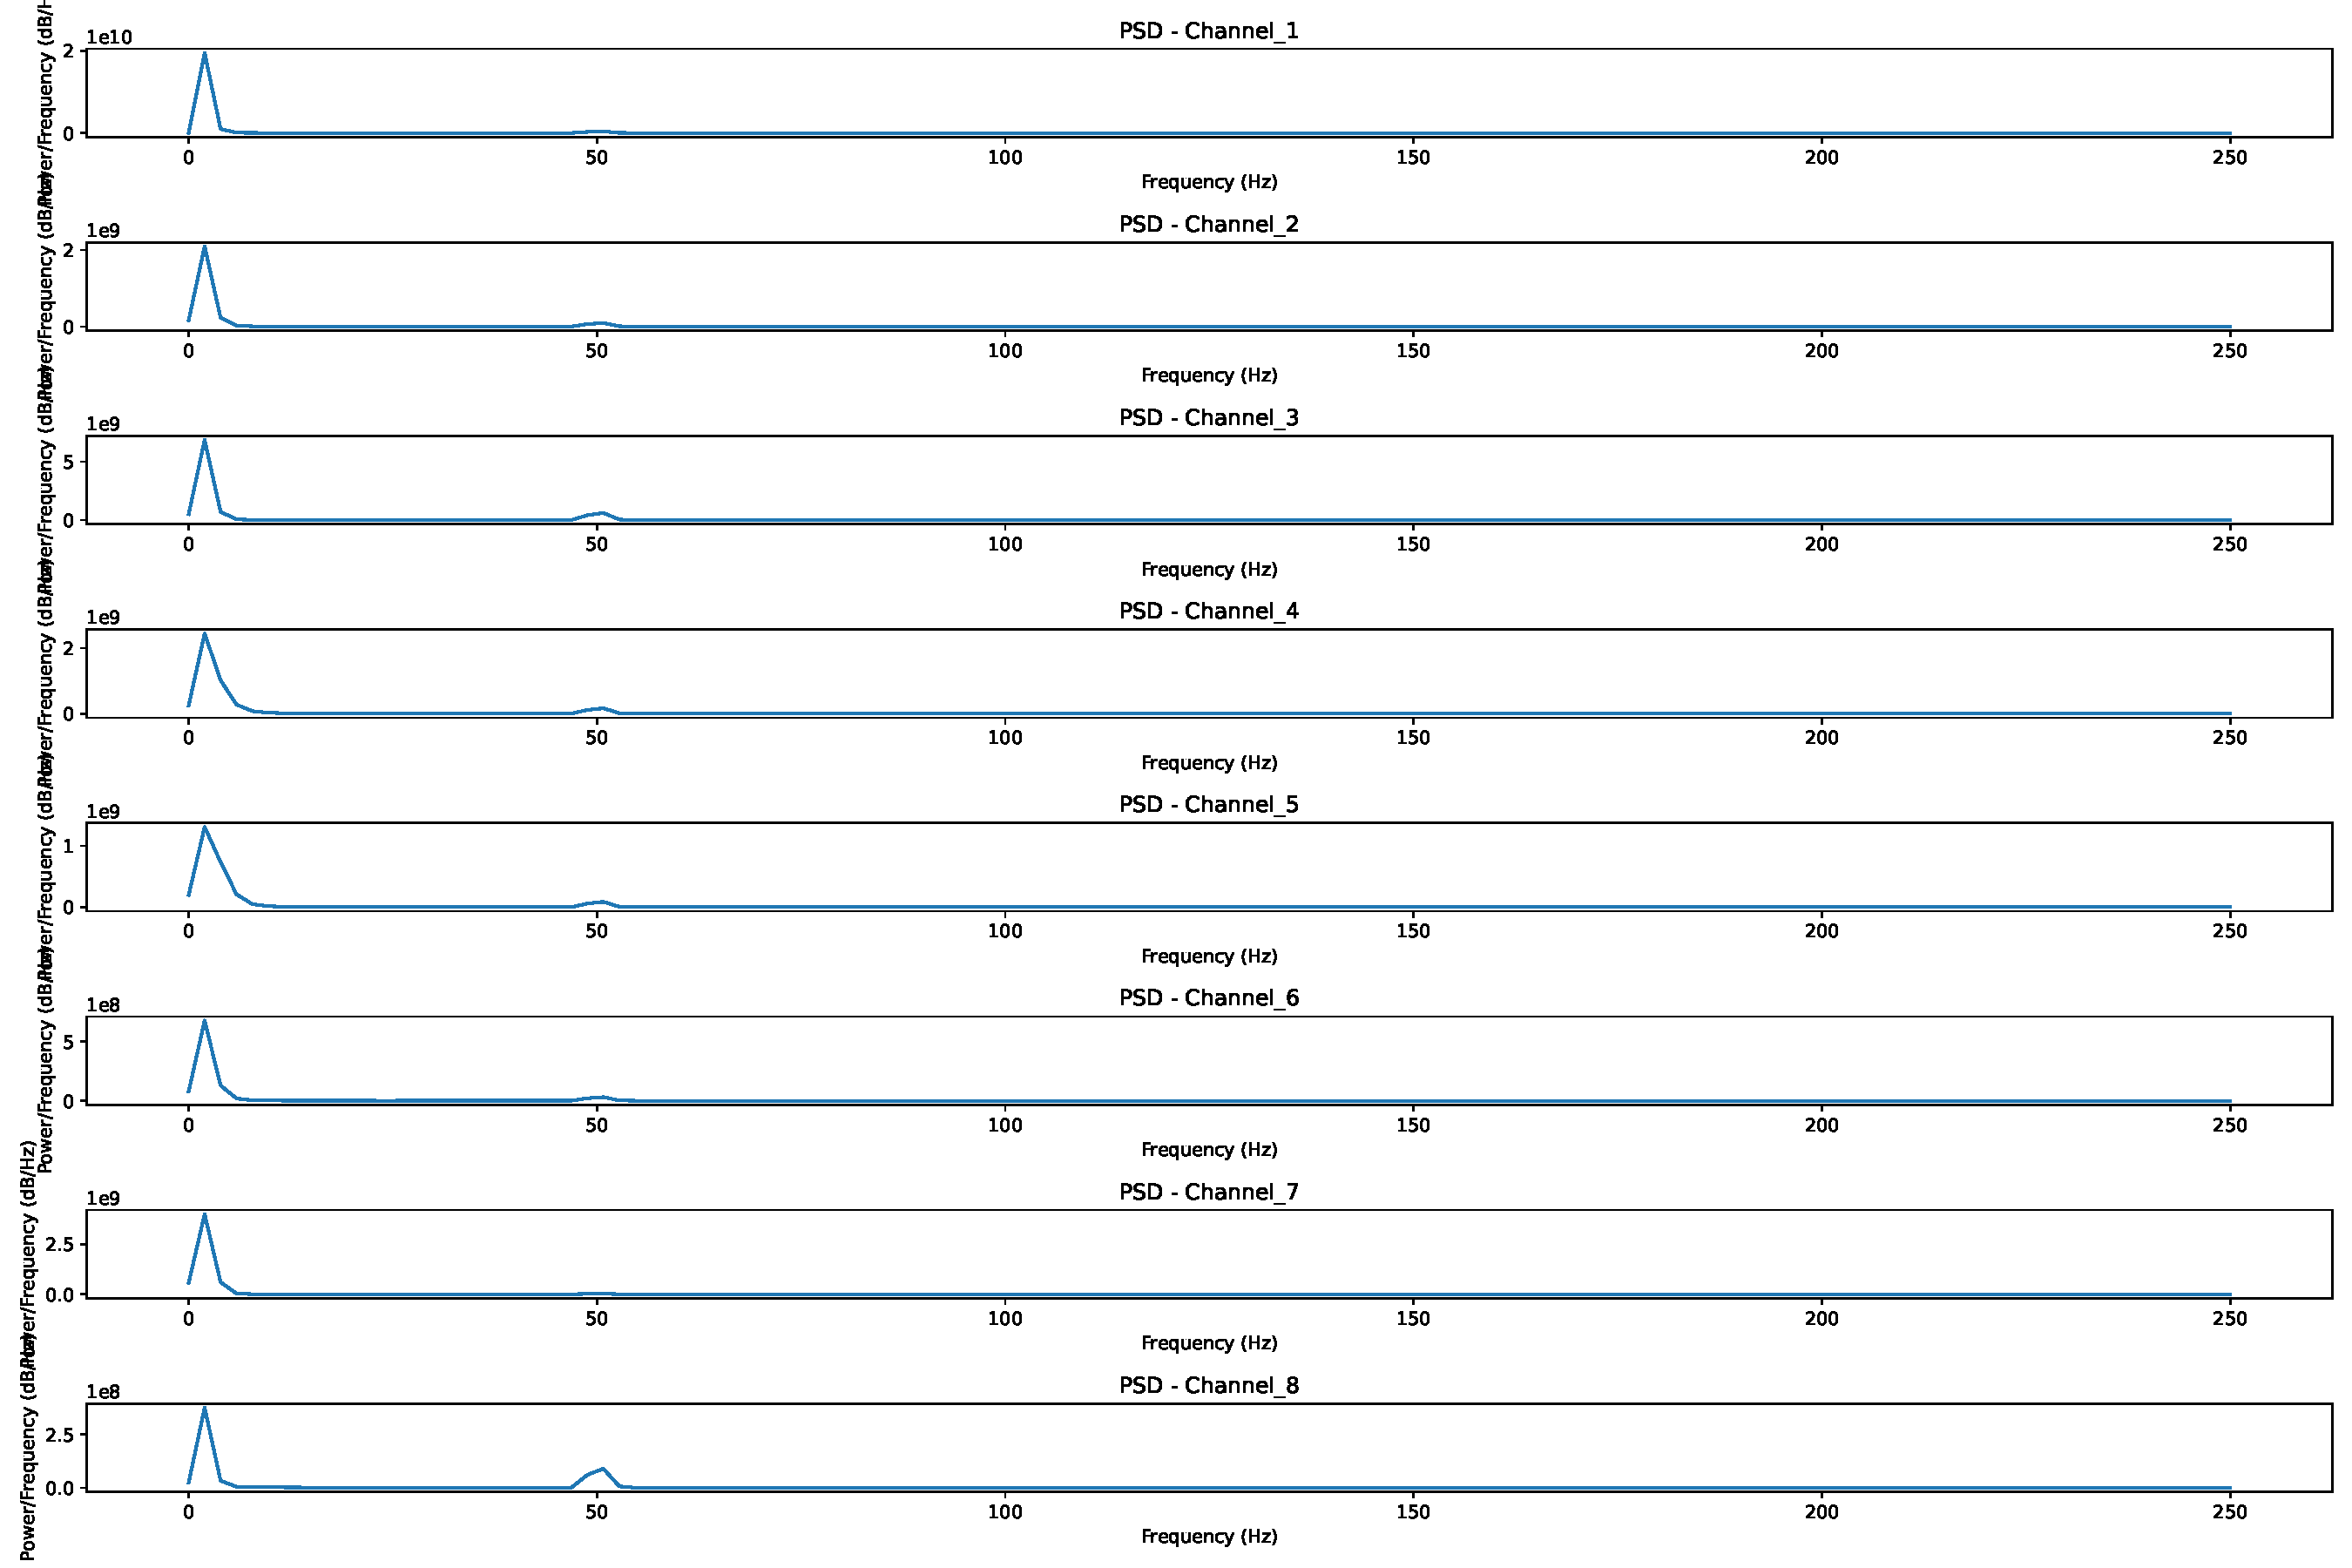
\includegraphics{eeg_files/figure-pdf/unnamed-chunk-3-3.pdf}

Power Spectral Density graph for each of the channels. \#\# Analysis

The EEG Signals are acquired from the above mentioned readings. We
recorded the raw EEG while the subject was relaxed with eyes closed. For
EEG recording with MP35 system, it was important to position the subject
away from the computer and to place MP35 away from the computer (set
aside or clip to subject).

In the ENOBIO recording, the subject's Power spectrum showed most of the
frequencies were around 10-15 Hz in majority of the channels. For
\texttt{channel\_8} some frequencies were found to be
\textasciitilde{}\(50Hz\).

\section{Result}\label{result-3}

The EEG Signal is acquired, recorded and analysed for statistical
parameters.

\bookmarksetup{startatroot}

\chapter{Audiometry}\label{audiometry}

\section{Aim}\label{aim-4}

\begin{quote}
To measure the hearing loss of a person and analyze the different types
of tests.
\end{quote}

\section{Theory}\label{theory-4}

Audiometry is a branch of audiology and the science of measuring hearing
acuity for variations in sound intensity and pitch and for tonal purity,
involving thresholds and differing frequencies. Typically, audiometric
tests determine a subject's hearing levels with the help of an
audiometer, but may also measure ability to discriminate between
different sound intensities, recognize pitch, or distinguish speech from
background noise.

Pure tone audiometry and audiograms - is a standardized hearing test in
which air conduction hearing thresholds in decibels (db) for a set of
fixed frequencies between 250 Hz and 8,000 Hz are plotted on an
audiogram for each ear independently. A separate set of measurements is
made for bone conduction. There is also high frequency Pure Tone
Audiometry covering the frequency range above 8000 Hz to 16,000 Hz.

Air and Bone conduction testing are methods of evaluating hearing loss
by comparing the perception of sounds transmitted by air or by bone:

\begin{itemize}
\item
  In air-conduction testing, a pure tone is presented via an earphone or
  a loudspeaker, and the signal travels through the outer, middle, and
  inner ear.
\item
  In bone-conduction testing, an electromechanical earphone is placed on
  the skull, and the signal bypasses the outer and middle ear. The Rinne
  test is a common example of air and bone conduction testing.
\end{itemize}

\section{Procedure}\label{procedure-4}

\begin{enumerate}
\def\labelenumi{\arabic{enumi}.}
\tightlist
\item
  Switch the computer ON.
\item
  Connect the USB (of Air conduction \& Bone conduction systems) to the
  Arphi Audiometry system.
\item
  Open Arphi 2001 Audiometry system on the Computer.
\item
  For Air Conduction click on ACR/ACL and for Bone Conduction click on
  BCR/BCL.
\item
  Ask the person to put on the respective instruments (headphones).
\item
  Select a Masking frequency.
\item
  Alter the frequency levels and dB levels \& allow the person to click
  every time they hear a sound → click on PLOT.
\item
  Analyze the graph for both right and left ear.
\item
  Click on save test → type the name \& save the data.
\item
  The same procedure can be repeated for both Air \& Bone Conduction
  Tests.
\end{enumerate}

\section{Observation}\label{observation-5}

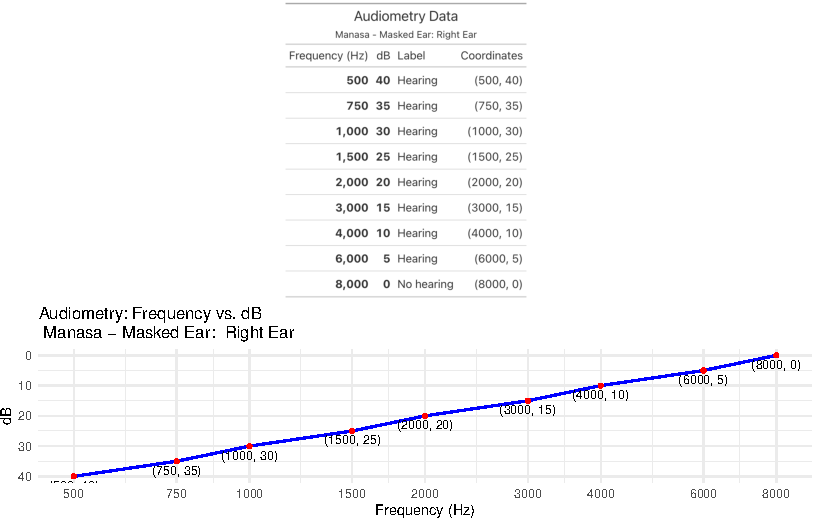
\includegraphics{audiometry_files/figure-pdf/unnamed-chunk-1-1.pdf}

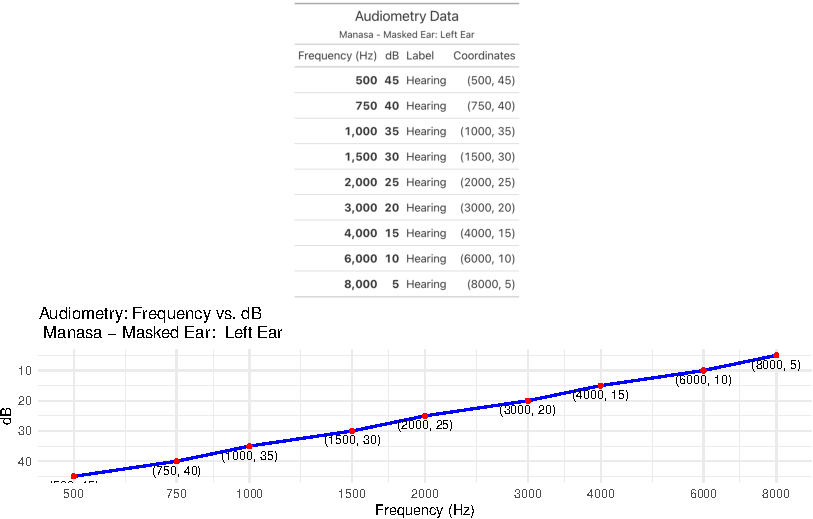
\includegraphics{audiometry_files/figure-pdf/unnamed-chunk-2-1.pdf}

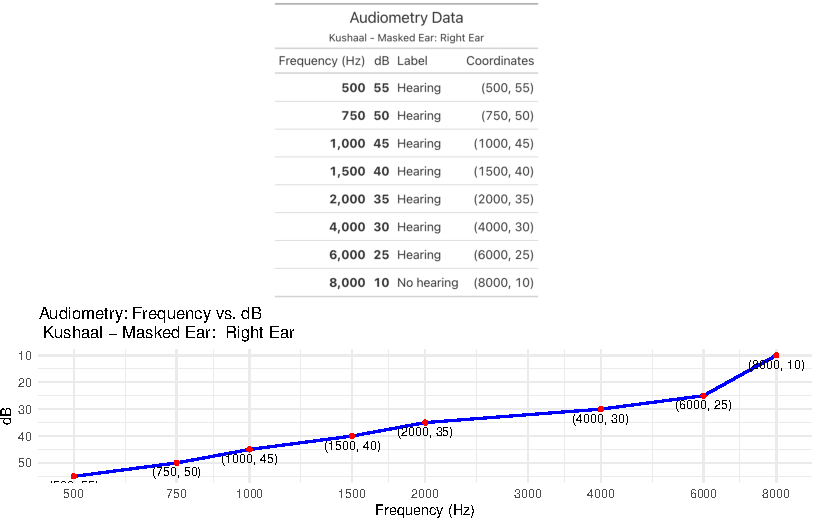
\includegraphics{audiometry_files/figure-pdf/unnamed-chunk-3-1.pdf}

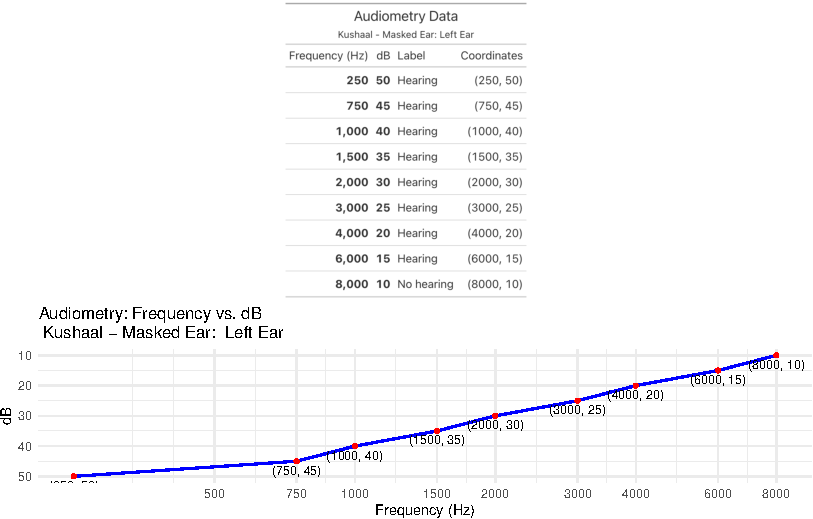
\includegraphics{audiometry_files/figure-pdf/unnamed-chunk-4-1.pdf}

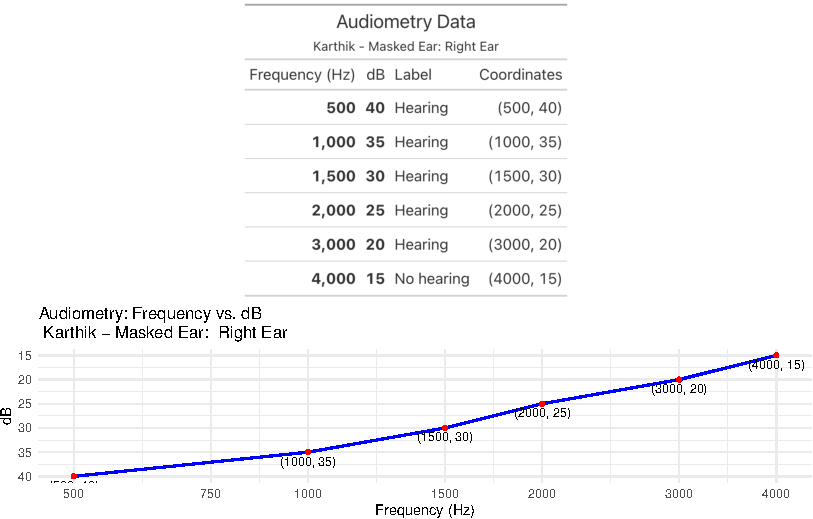
\includegraphics{audiometry_files/figure-pdf/unnamed-chunk-5-1.pdf}

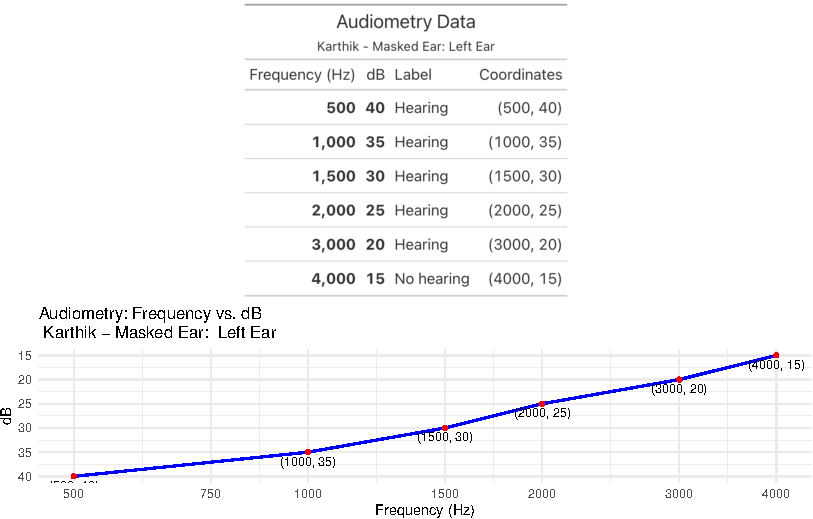
\includegraphics{audiometry_files/figure-pdf/unnamed-chunk-6-1.pdf}

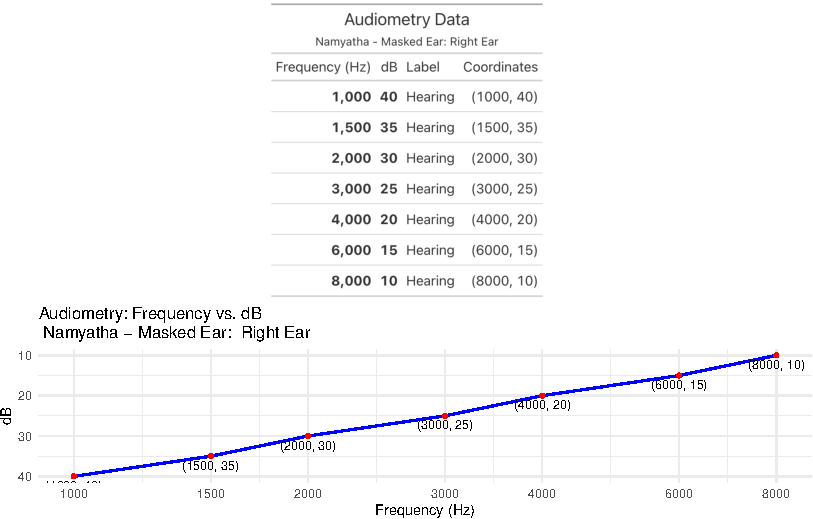
\includegraphics{audiometry_files/figure-pdf/unnamed-chunk-7-1.pdf}

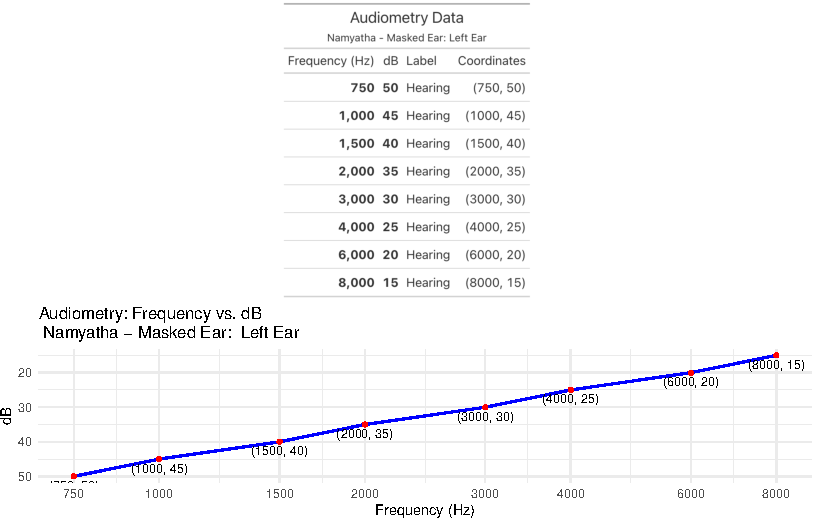
\includegraphics{audiometry_files/figure-pdf/unnamed-chunk-8-1.pdf}

\section{Analysis}\label{analysis-3}

Calculation of the hearing threshold of a person.

Hearing threshold : It is the lowest threshold of acoustic pressure
sensation, possible to perceive by an organism. It is the sound level
below which a person's ear is unable to detect any sound. For adults, 0
dB is the reference level. A threshold shift is an increase in the
hearing threshold for a particular sound frequency.

\textbf{Female subjects in the study have hearing threshold of 0dB,
while the Male participants in the study have 10 and 15dB.}

\section{Results}\label{results}

The Air Conduction method is analysed.

\bookmarksetup{startatroot}

\chapter{ECG Waveform Simulation}\label{ecg-waveform-simulation}

\section{Aim}\label{aim-5}

\begin{enumerate}
\def\labelenumi{\arabic{enumi}.}
\tightlist
\item
  To understand normal ECG waveform.
\item
  To understand noise associated with ECG measurement i.e.~line
  Frequency and baseline wandering
\item
  To understand various abnormalities associated with ECG pattern.
\end{enumerate}

\section{Pre Requisites}\label{pre-requisites}

\begin{itemize}
\tightlist
\item
  Knowledge of various physiological system.
\item
  Tools like NI LabVIEW and MATLAB.
\end{itemize}

\section{Theory}\label{theory-5}

Human heart is a muscle that works continuously, much like a pump. Each
beat of human heart is set in motion by an electrical signal from within
heart muscle. The electrical activity of heart is recorded by an
electrocardiogram, known as an EKG or ECG.

Human heart's electrical system controls all the events that occur when
heart pumps blood. The electrical system also is called the cardiac
conduction system.

\subsection{P Wave}\label{p-wave}

The P wave represents the wave of depolarization that spreads from the
SA node throughout the atria, and is usually 0.08 to 0.1 seconds (80-100
ms) in duration. The brief isoelectric (zero voltage) period after the P
wave represents the time in which the impulse is traveling within the AV
node (where the conduction velocity is greatly retarded) and the bundle
of His. Atrial rate can be calculated by determining the time interval
between P waves.

\subsection{QRS Complex}\label{qrs-complex}

The QRS complex represents ventricular depolarization. Ventricular rate
can be calculated by determining the time interval between QRS
complexes. The duration of the QRS complex is normally 0.06 to 0.1
seconds. This relatively short duration indicates that ventricular
depolarization normally occurs very rapidly. If the QRS complex is
prolonged (\textgreater{} 0.1 sec), conduction is impaired within the
ventricles. This can occur with bundle branch blocks or whenever a
ventricular foci(abnormal pacemaker site) becomes the pacemaker driving
the ventricle. Such an ectopic foci nearly always results in impulses
being conducted over slower pathways within the heart, thereby
increasing the time for depolarization and the duration of the QRS
complex.

\subsection{ST Segment}\label{st-segment}

The isoelectric period (ST segment) following the QRS is the time at
which the entire ventricle is depolarized and roughly corresponds to the
plateau phase of the ventricular action potential. The ST segment is
important in the diagnosis of ventricular ischemia or hypoxia because
under those conditions, the ST segment can become either depressed or
elevated.

\subsection{T Wave}\label{t-wave}

The T wave represents ventricular repolarization and is longer in
duration than depolarization (i.e., conduction of the repolarization
wave is slower than the wave of depolarization). Sometimes a small
positive U wave may be seen following the T wave (not shown in figure
1). This wave represents the last remnants of ventricular
repolarization. Inverted or prominent U waves indicate underlying
pathology or conditions affecting repolarization.

\subsection{QT Interval}\label{qt-interval}

The Q-T interval represents the time for both ventricular depolarization
and repolarization to occur, and therefore roughly estimates the
duration of an average ventricular action potential. This interval can
range from 0.2 to 0.4 seconds depending upon heart rate. At high heart
rates, ventricular action potentials shorten in duration, which
decreases the Q-T interval. Because prolonged Q-T intervals can be
diagnostic for susceptibility to certain types of tachyarrhythmias, it
is important to determine if a given Q-T interval is excessively long.

\section{Simulation}\label{simulation}

\begin{figure}[H]

{\centering 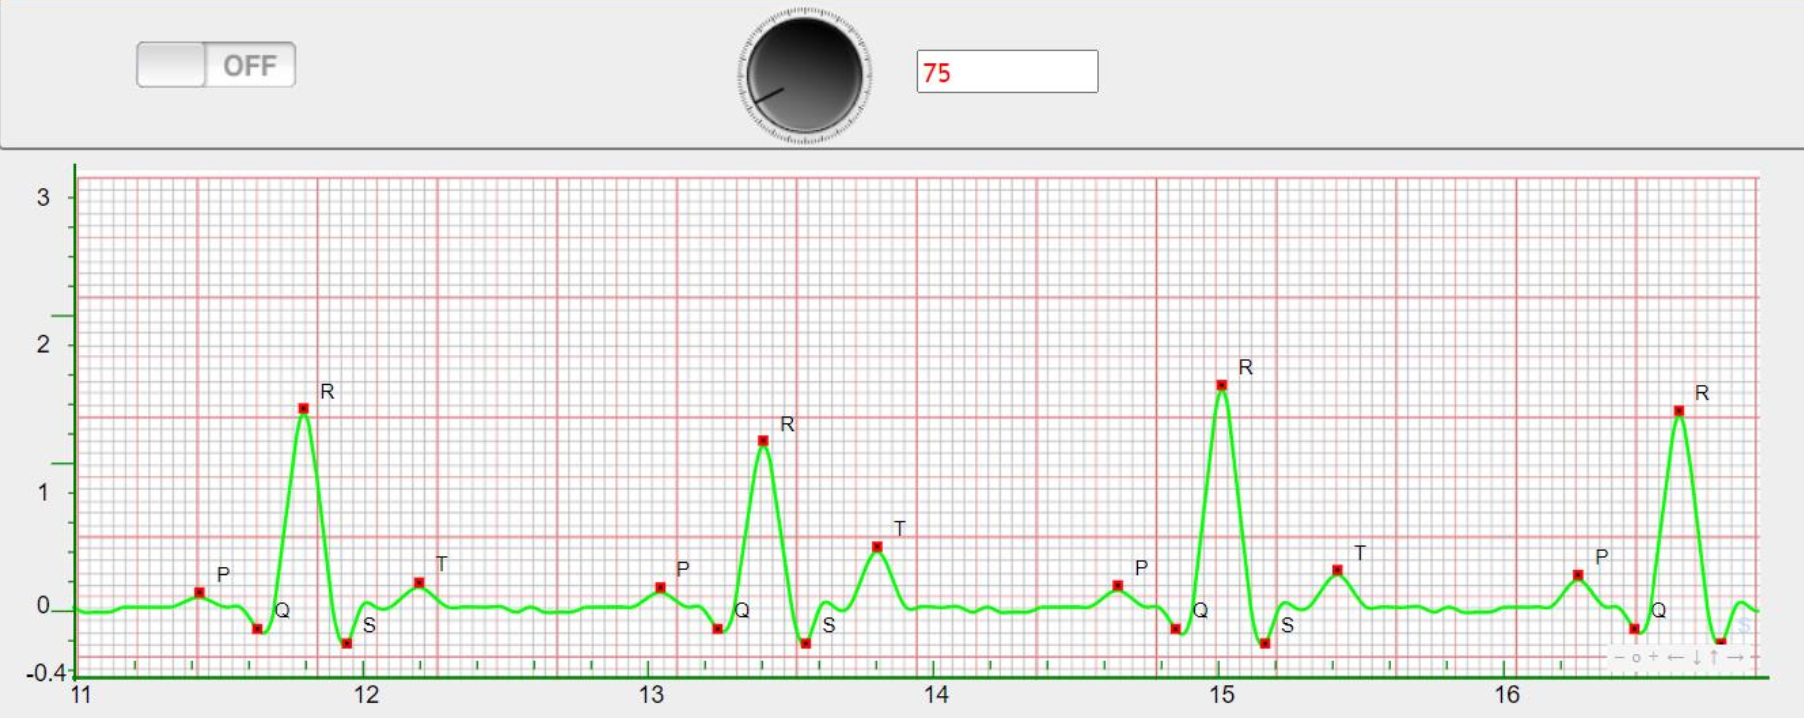
\includegraphics{images/clipboard-2660105563.png}

}

\caption{Normal ECG Waveform}

\end{figure}%%
\begin{figure}[H]

{\centering 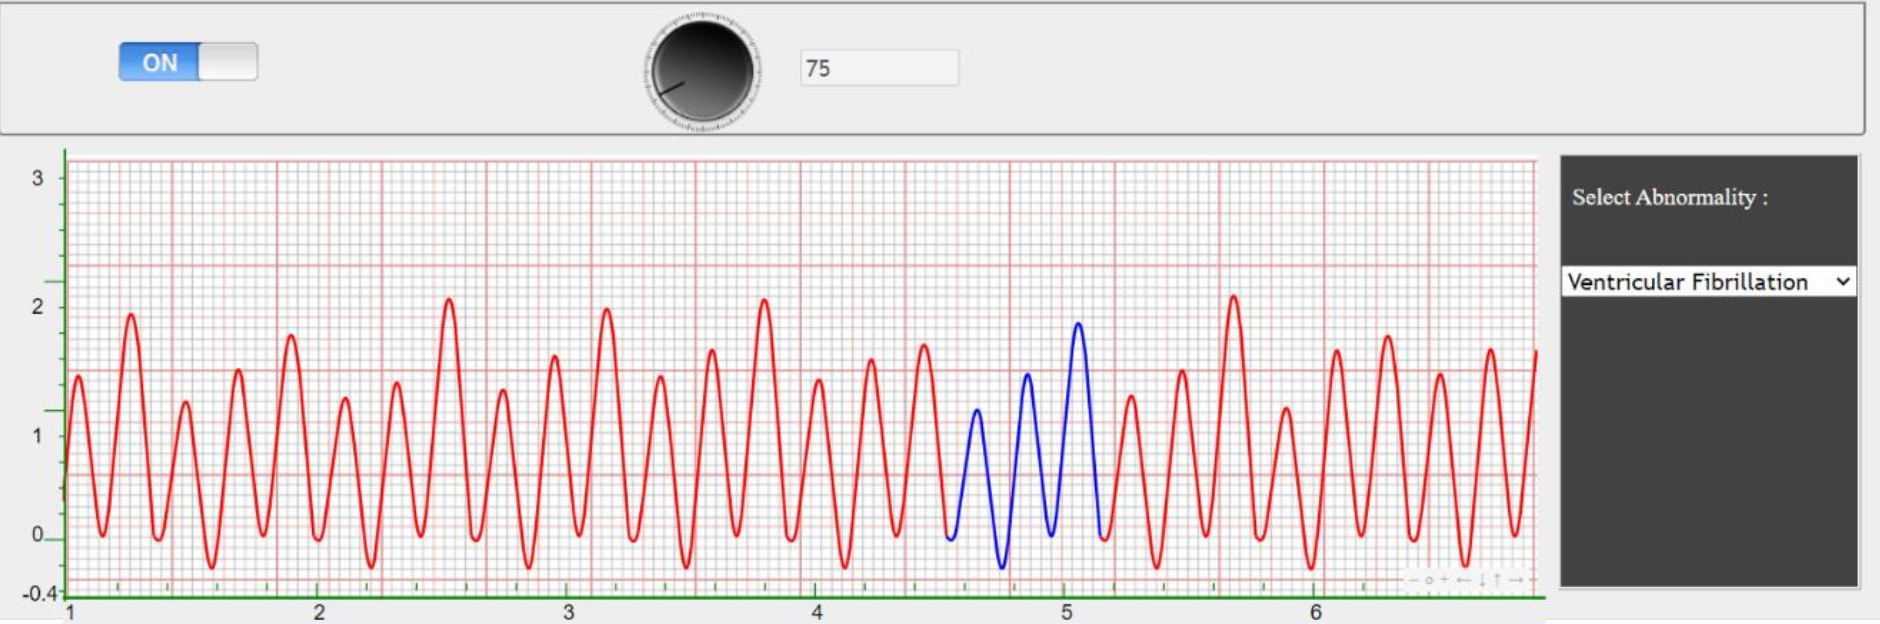
\includegraphics{images/clipboard-2256462463.png}

}

\caption{Abnormal ECG Waveform}

\end{figure}%%
\begin{figure}[H]

{\centering 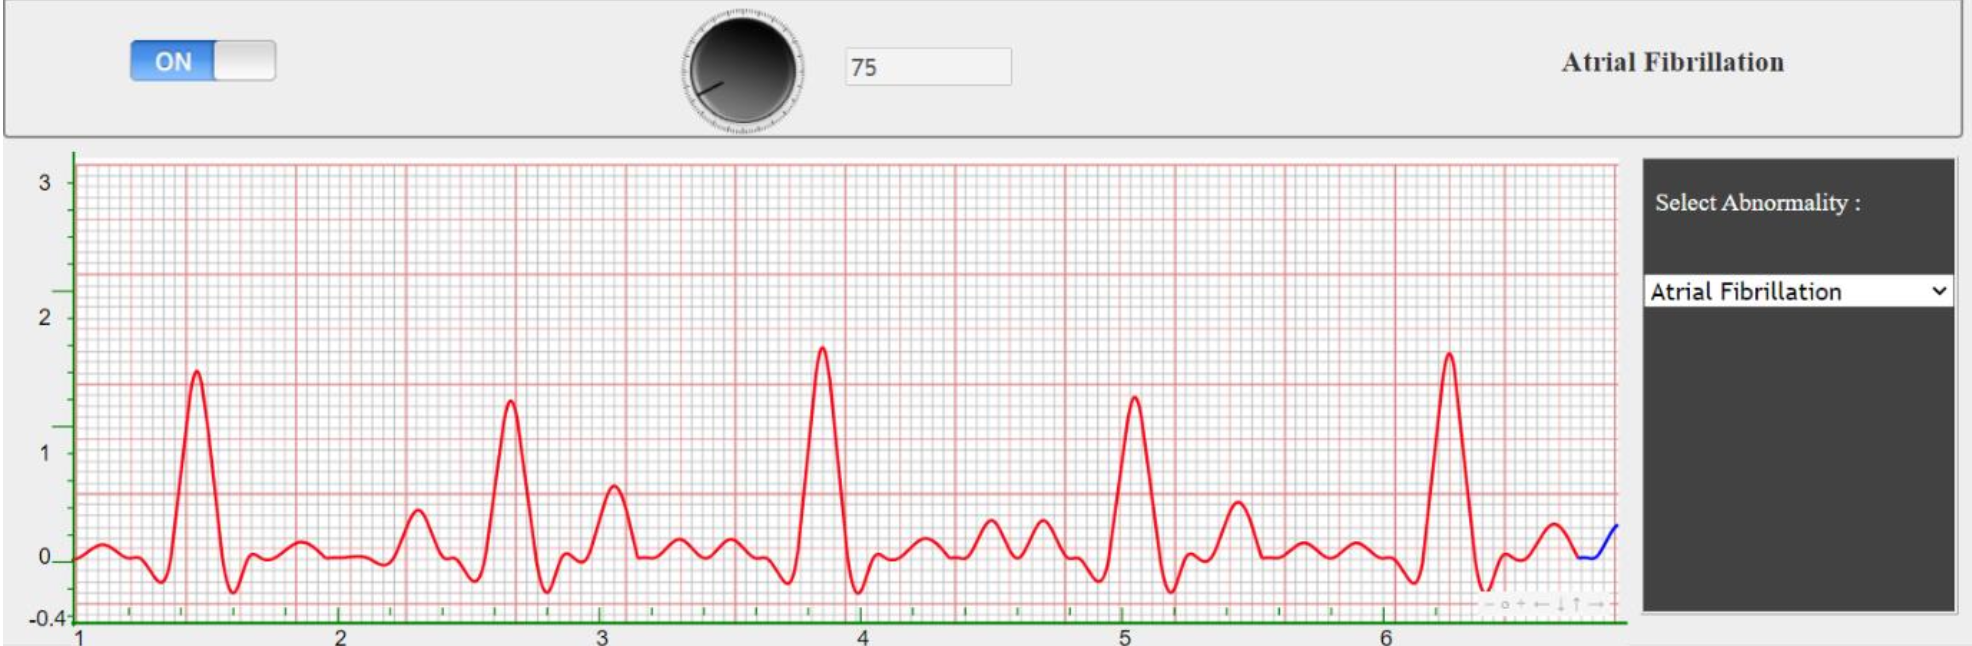
\includegraphics{images/clipboard-2993141644.png}

}

\caption{Abnormal Moving ECG Waveform}

\end{figure}%%
\begin{figure}[H]

{\centering 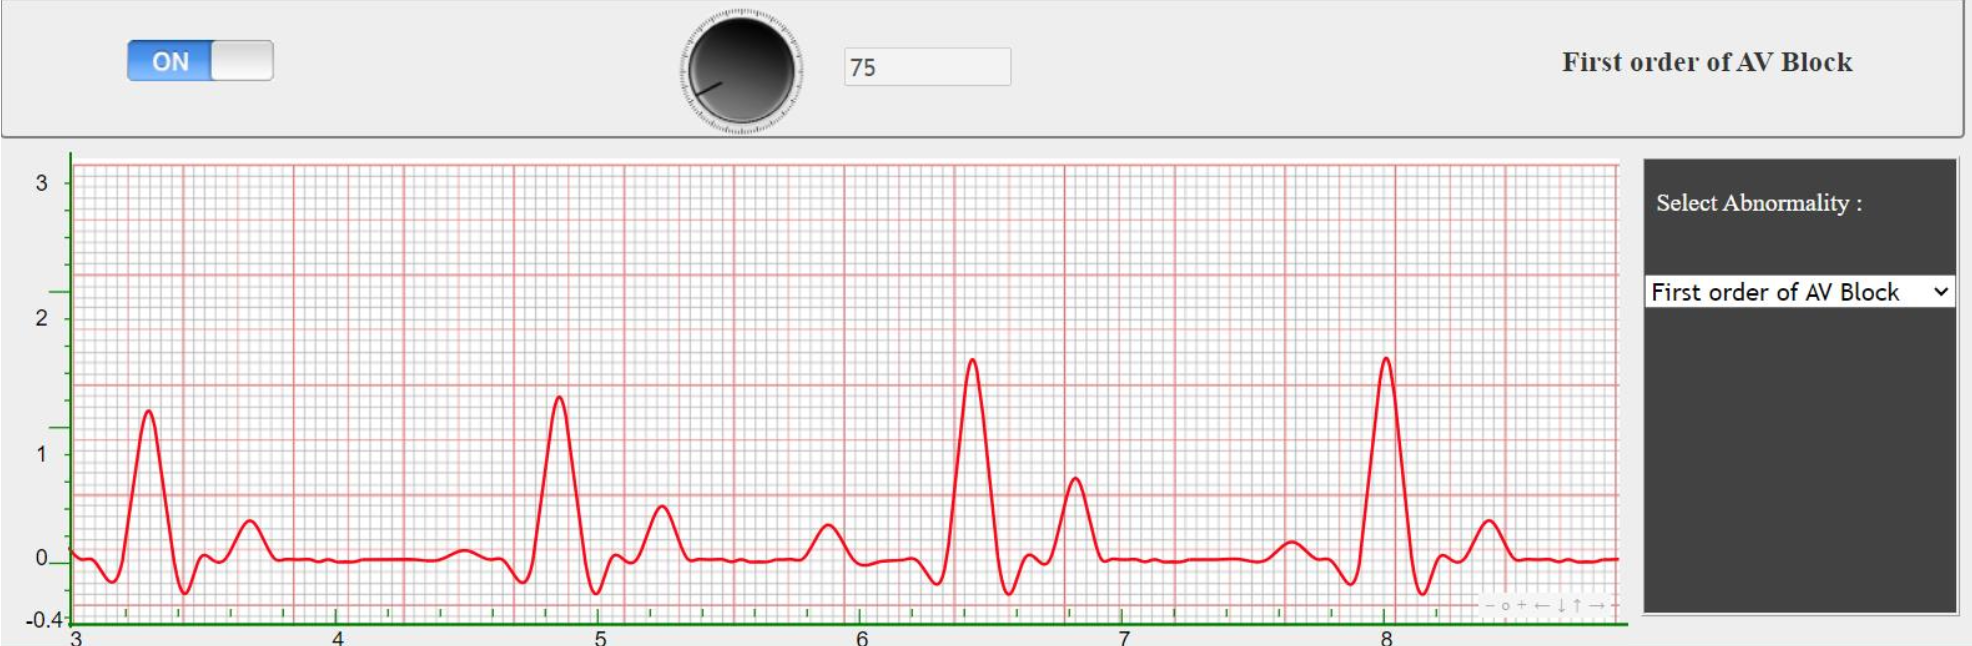
\includegraphics{images/clipboard-3470925149.png}

}

\caption{Abnormal ECG Main Plate}

\end{figure}%%
\begin{figure}[H]

{\centering 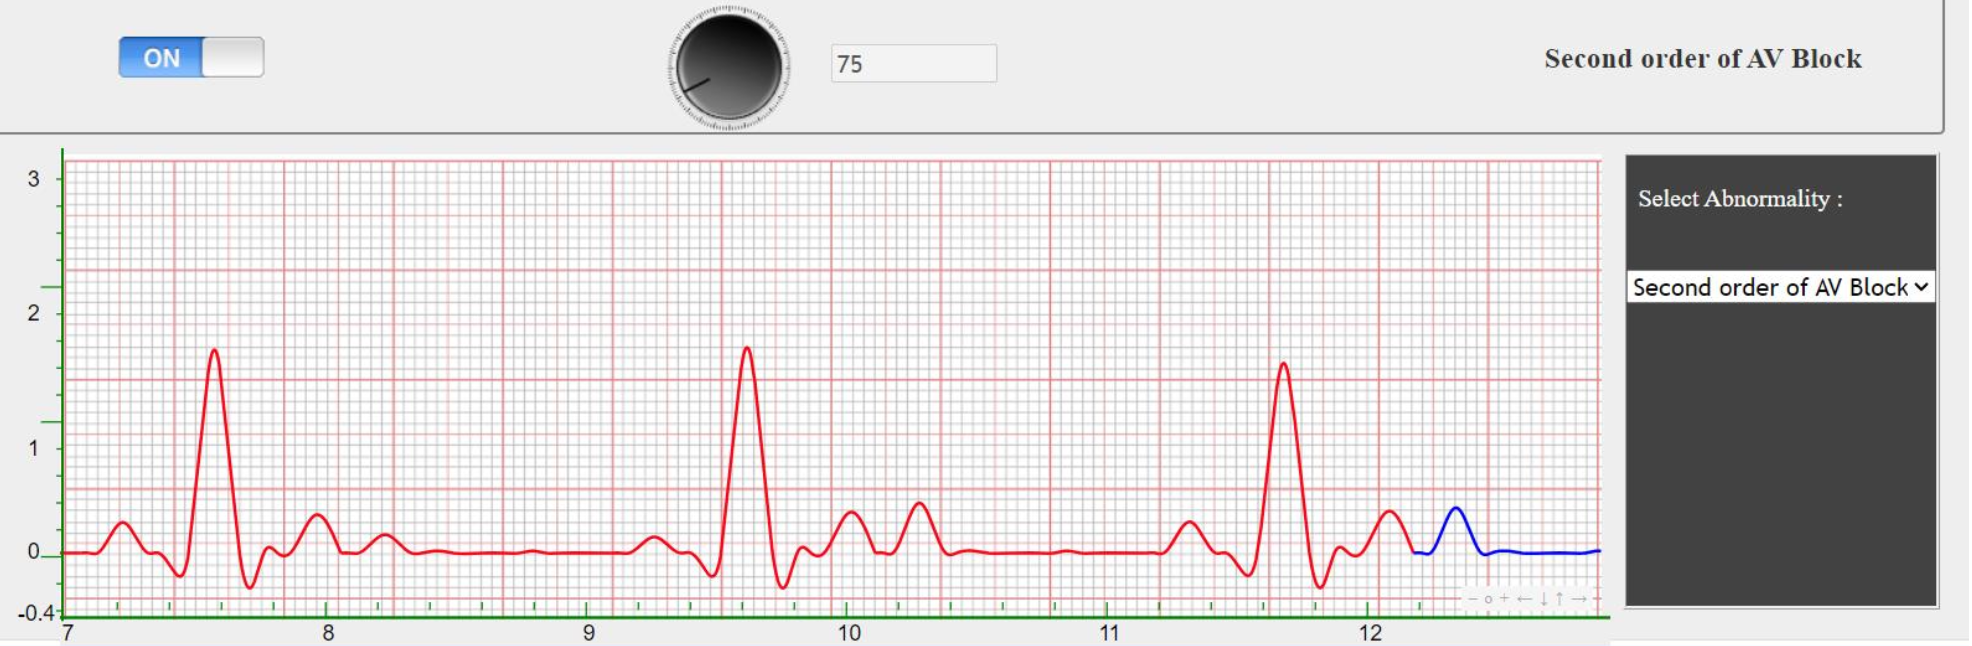
\includegraphics{images/clipboard-3576673599.png}

}

\caption{Abnormal ECG Main Plate: Moving waveform}

\end{figure}%

\section{Result}\label{result-4}

\begin{quote}
Thus, ECG Waveforms were simulated to observe the normal and abnormal
patterns.
\end{quote}

\bookmarksetup{startatroot}

\chapter{EEG Waveform Simulation}\label{eeg-waveform-simulation}

\section{Aim}\label{aim-6}

\begin{enumerate}
\def\labelenumi{\arabic{enumi}.}
\tightlist
\item
  To understand normal EEG pattern.
\item
  To understand various abnormalities associated with EEG.
\item
  To assist in studying sleep patterns.
\item
  To assist in diagnosing mental disorders.
\end{enumerate}

\section{Pre Requisites}\label{pre-requisites-1}

\begin{itemize}
\tightlist
\item
  Understanding of Central Nervous System
\item
  Tools like NI LabVIEW and MATLAB
\end{itemize}

\section{Theory}\label{theory-6}

The electroencephalogram (EEG) is a unique and valuable measure of the
brain's electrical function. It is a graphic display of a difference in
voltages from two sites of brain function recorded over time.
Electroencephalography (EEG) involves the study of recording these
electrical signals that are generated by the brain.

\subsection{10-20 Electrode Positioning:}\label{electrode-positioning}

The 10-20 system avoids both eyeball placement and considers some
constant distances by using specific anatomic landmarks from which the
measurement would be made and then uses 10 or 20\% of that specified
distance as the electrode interval. The odd electrodes are on the left
and the even ones on the right.

There are five major brain waves distinguished by their different
frequency ranges. These frequency bands from low to high frequencies
respectively are: delta (δ), theta (θ), alpha (α), beta (β) and gamma
(γ).

\section{Simulation}\label{simulation-1}

\begin{center}
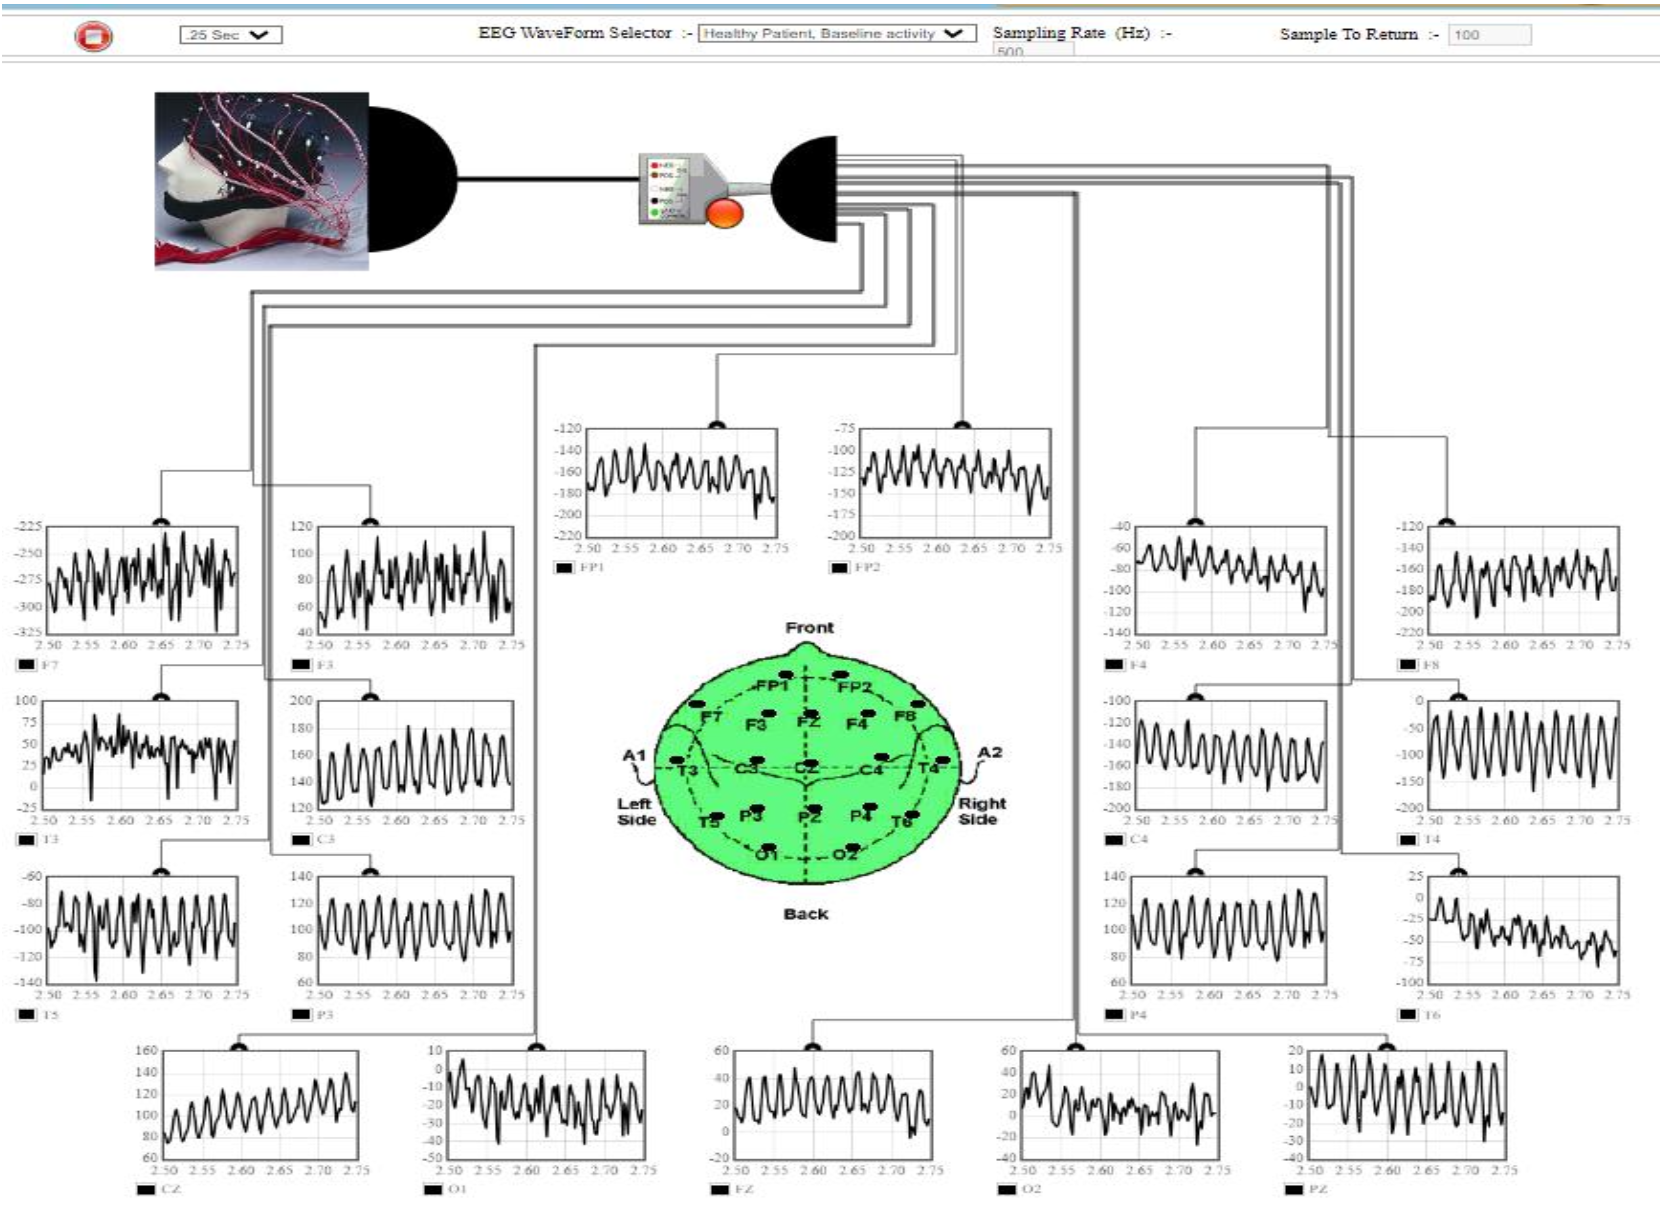
\includegraphics[width=5.6875in,height=5.28125in]{images/clipboard-2845690509.png}
\end{center}

\begin{center}
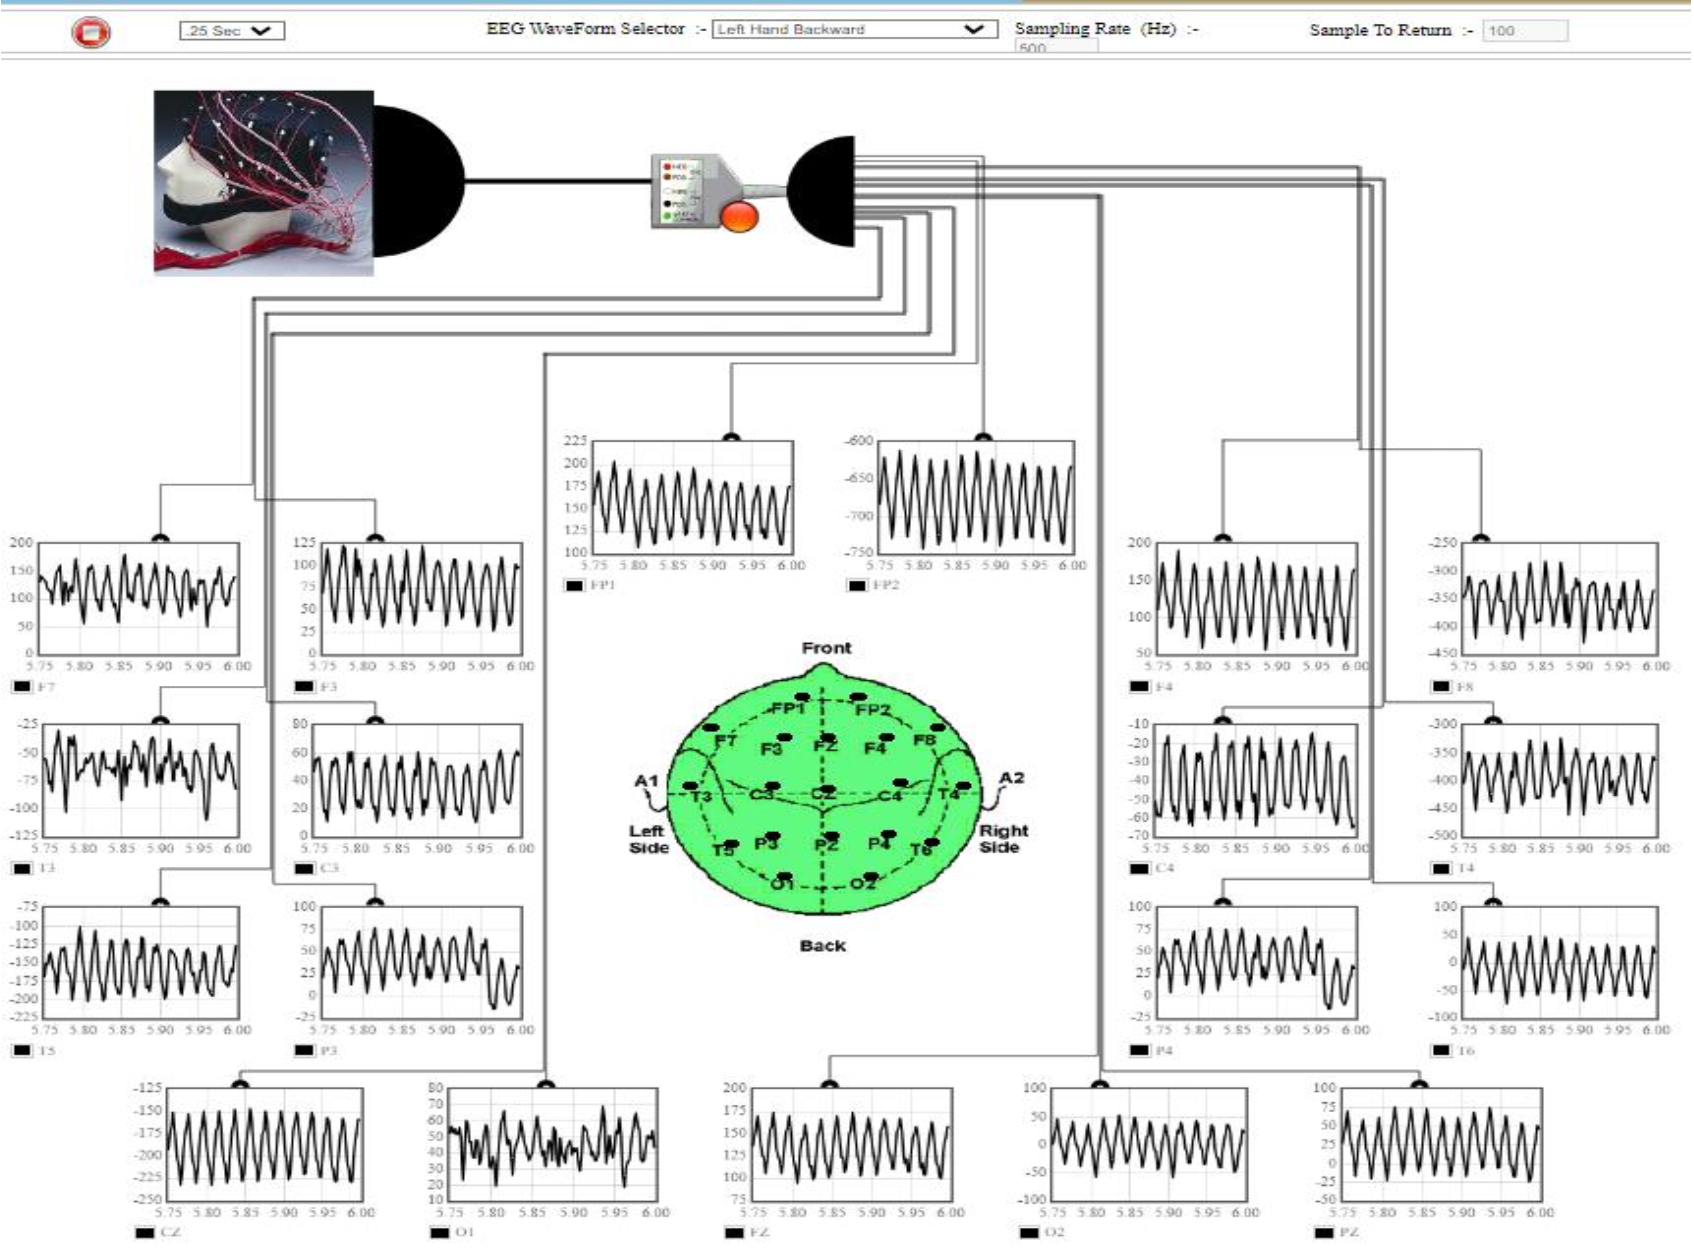
\includegraphics[width=5.66667in,height=4.89583in]{images/clipboard-8096195.png}
\end{center}

\begin{center}
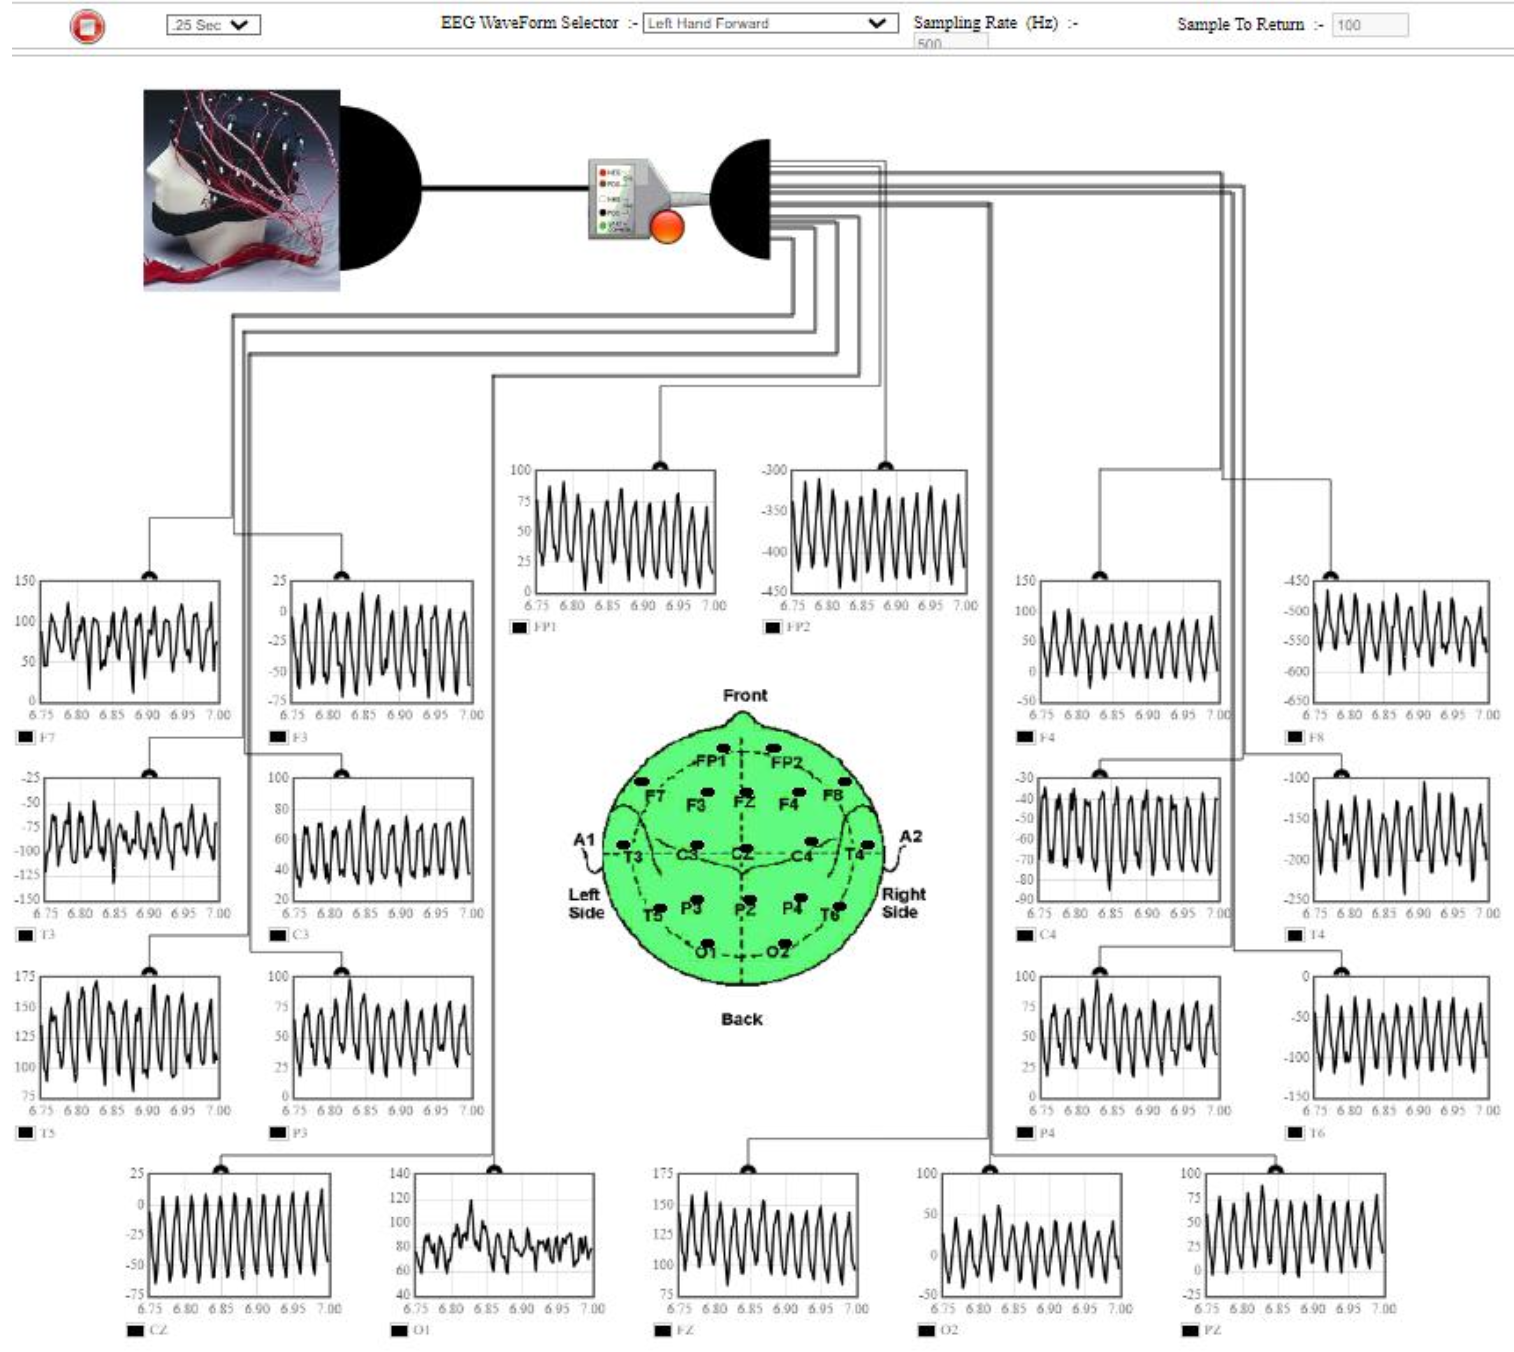
\includegraphics[width=5.11458in,height=\textheight]{images/clipboard-2354709684.png}
\end{center}

\begin{center}
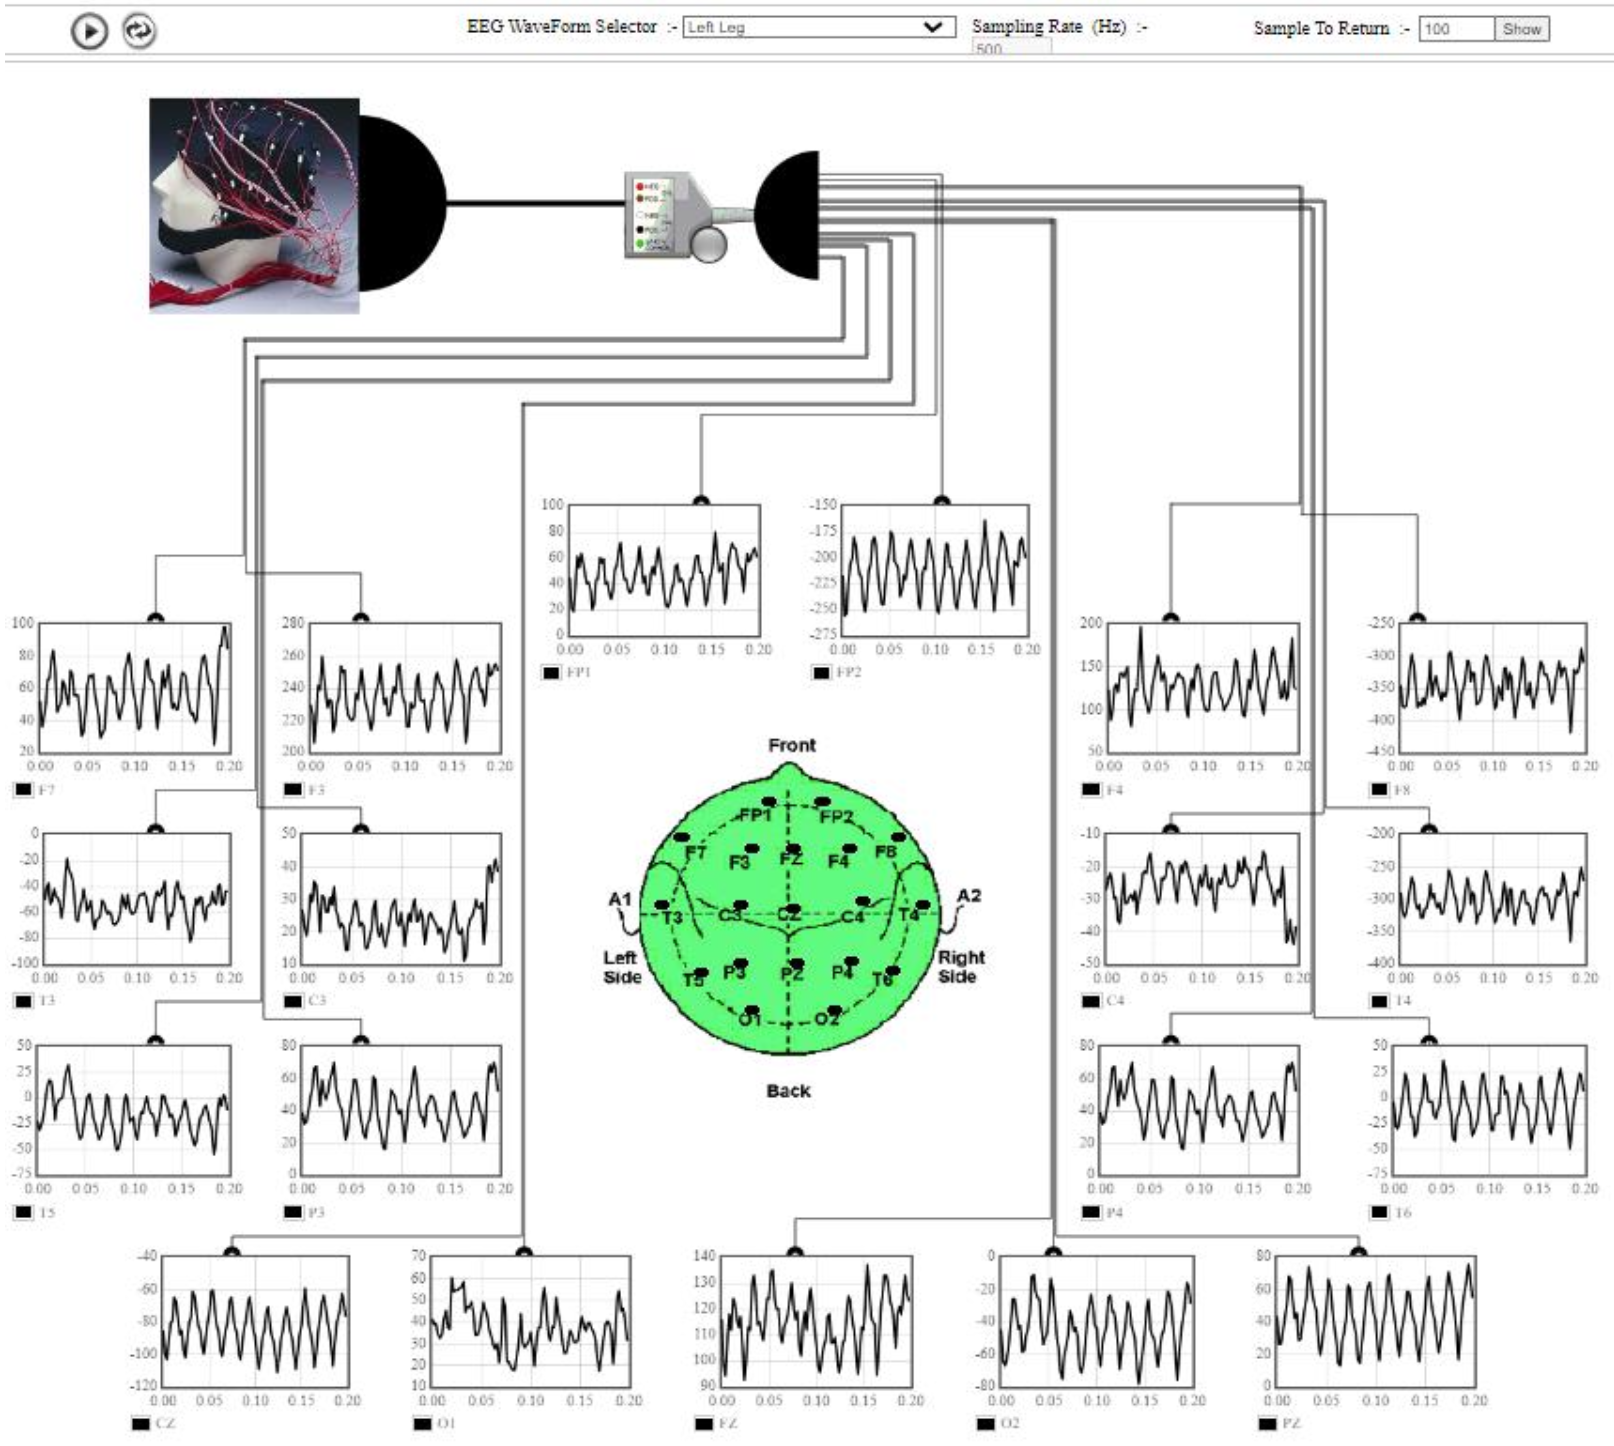
\includegraphics[width=4.41667in,height=\textheight]{images/clipboard-2400029708.png}
\end{center}

\begin{center}
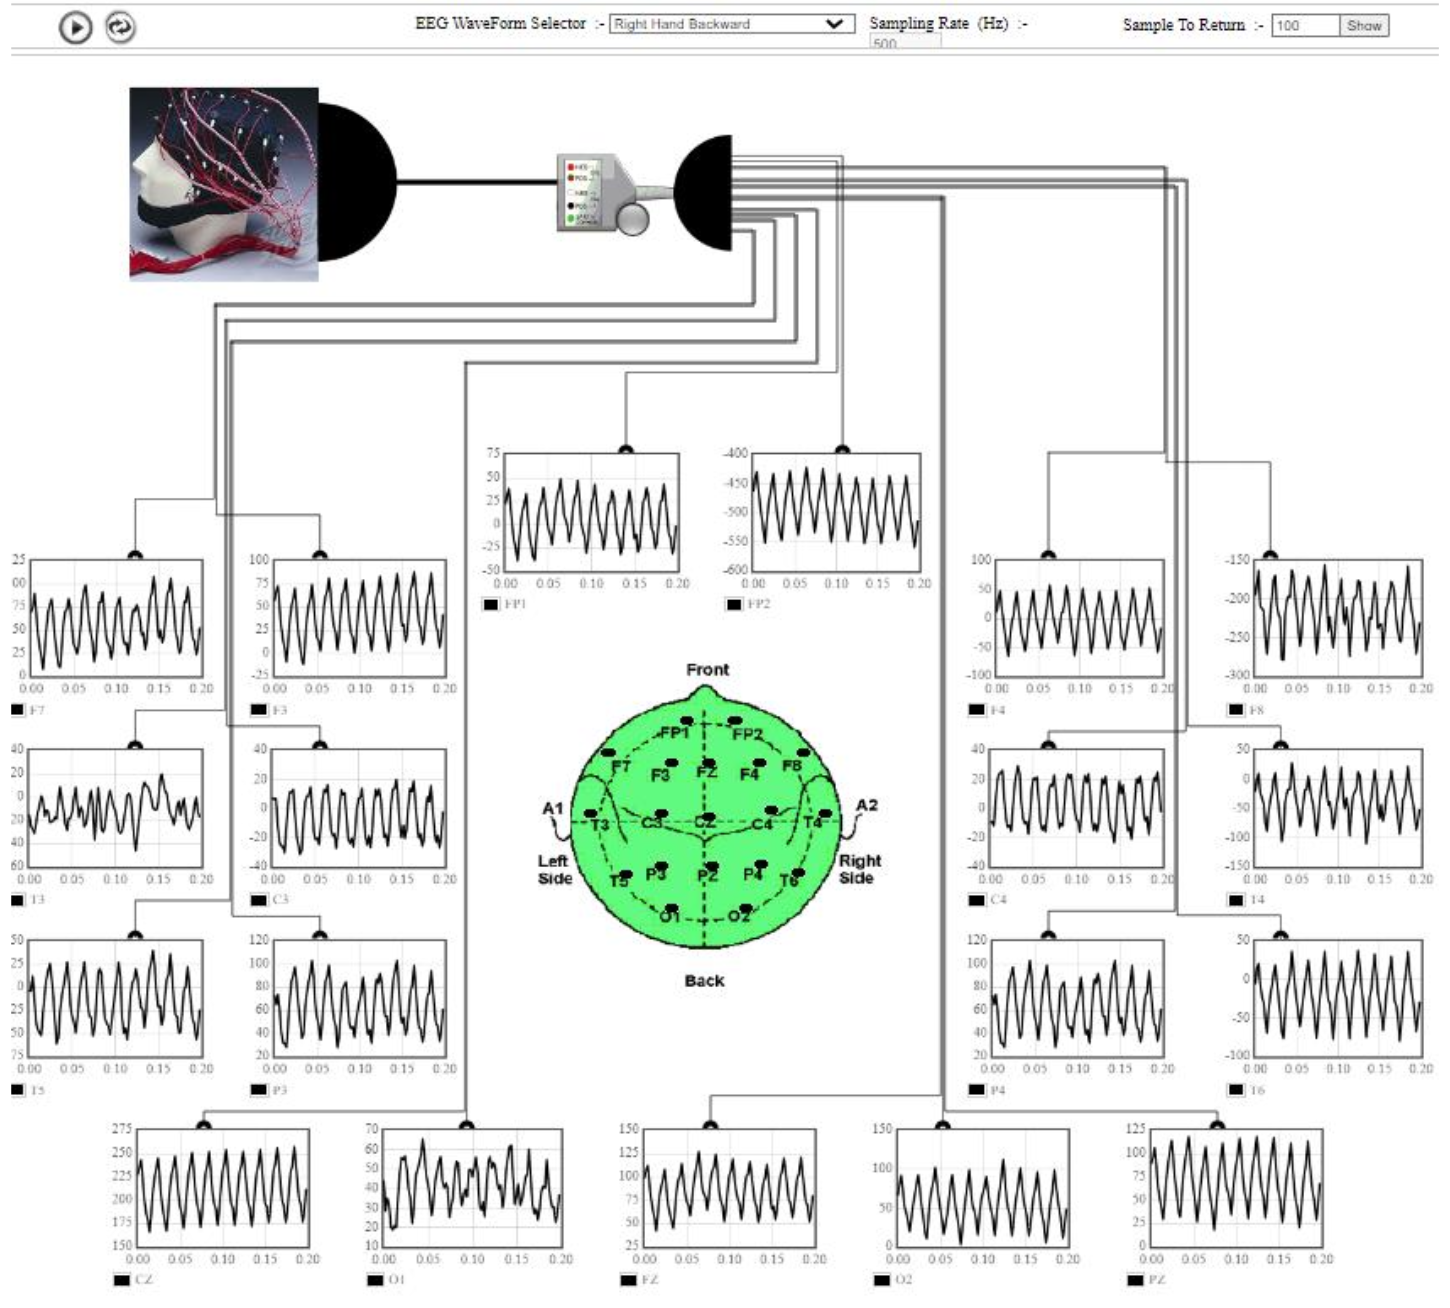
\includegraphics[width=4.44792in,height=3.90625in]{images/clipboard-13240665.png}
\end{center}

\begin{center}
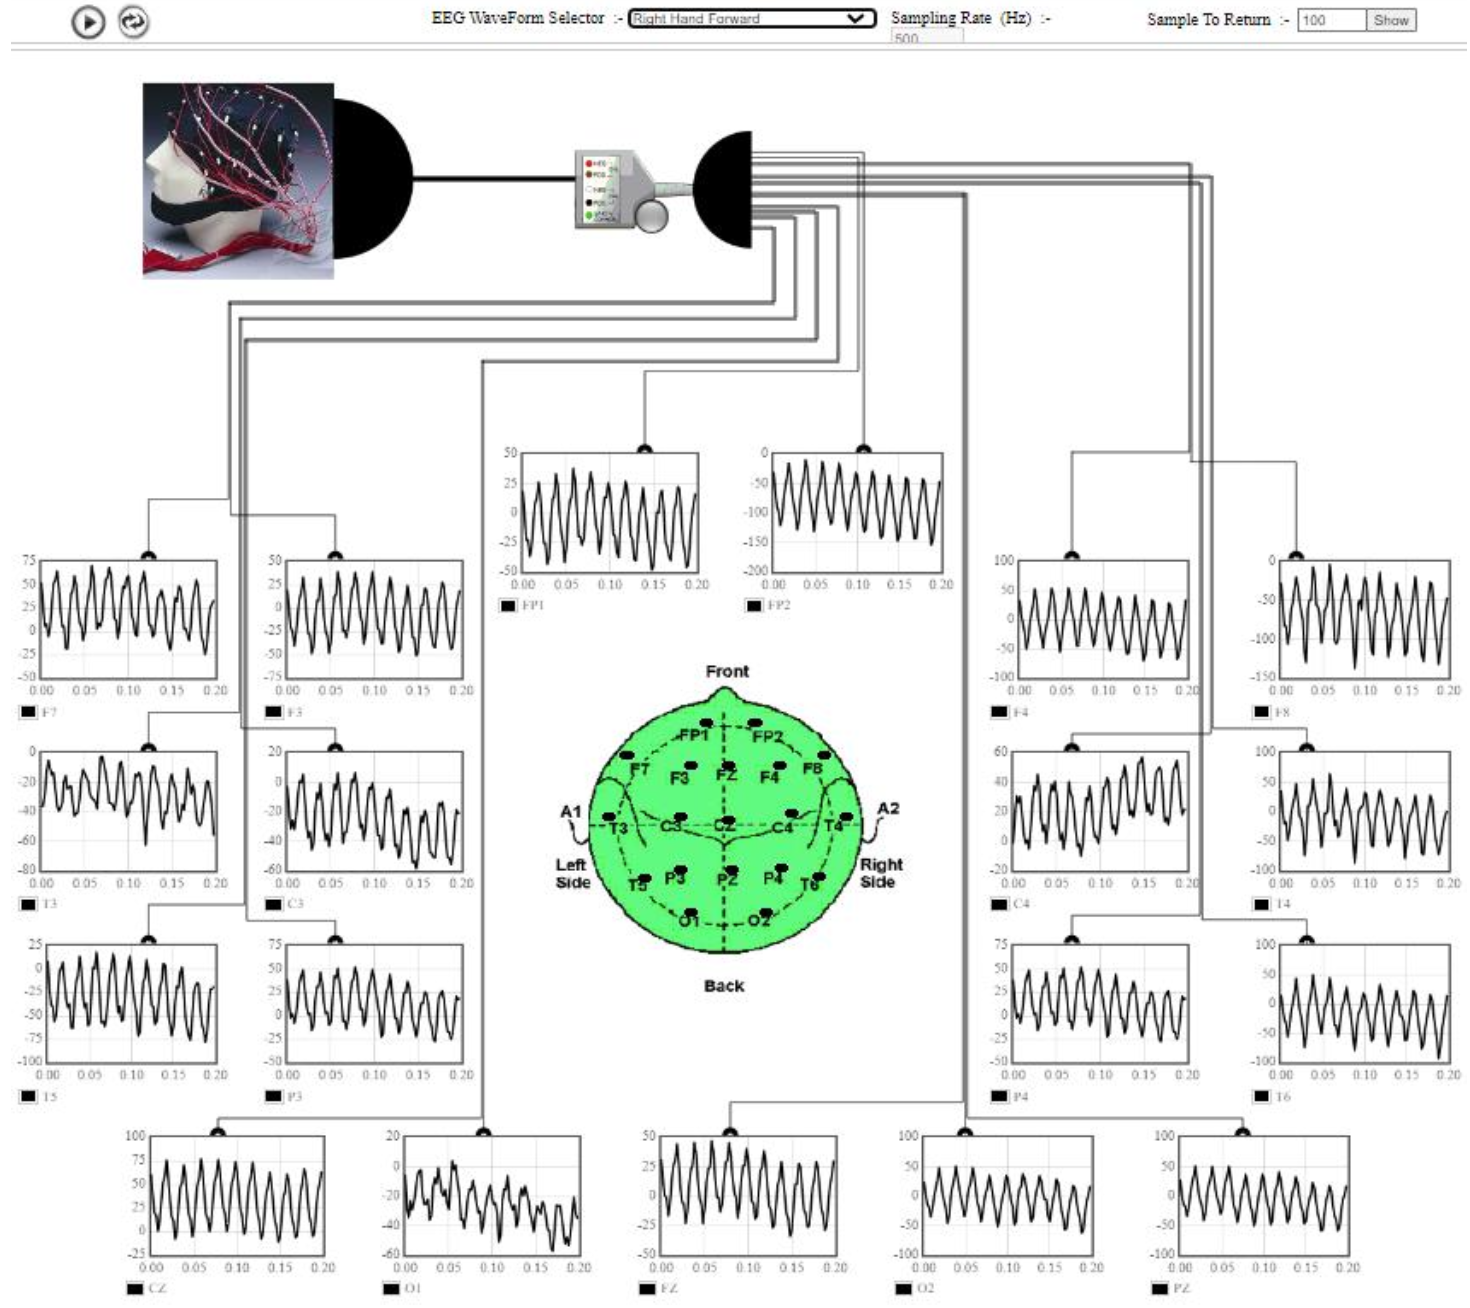
\includegraphics[width=4.83333in,height=\textheight]{images/clipboard-3969083955.png}
\end{center}

\begin{center}
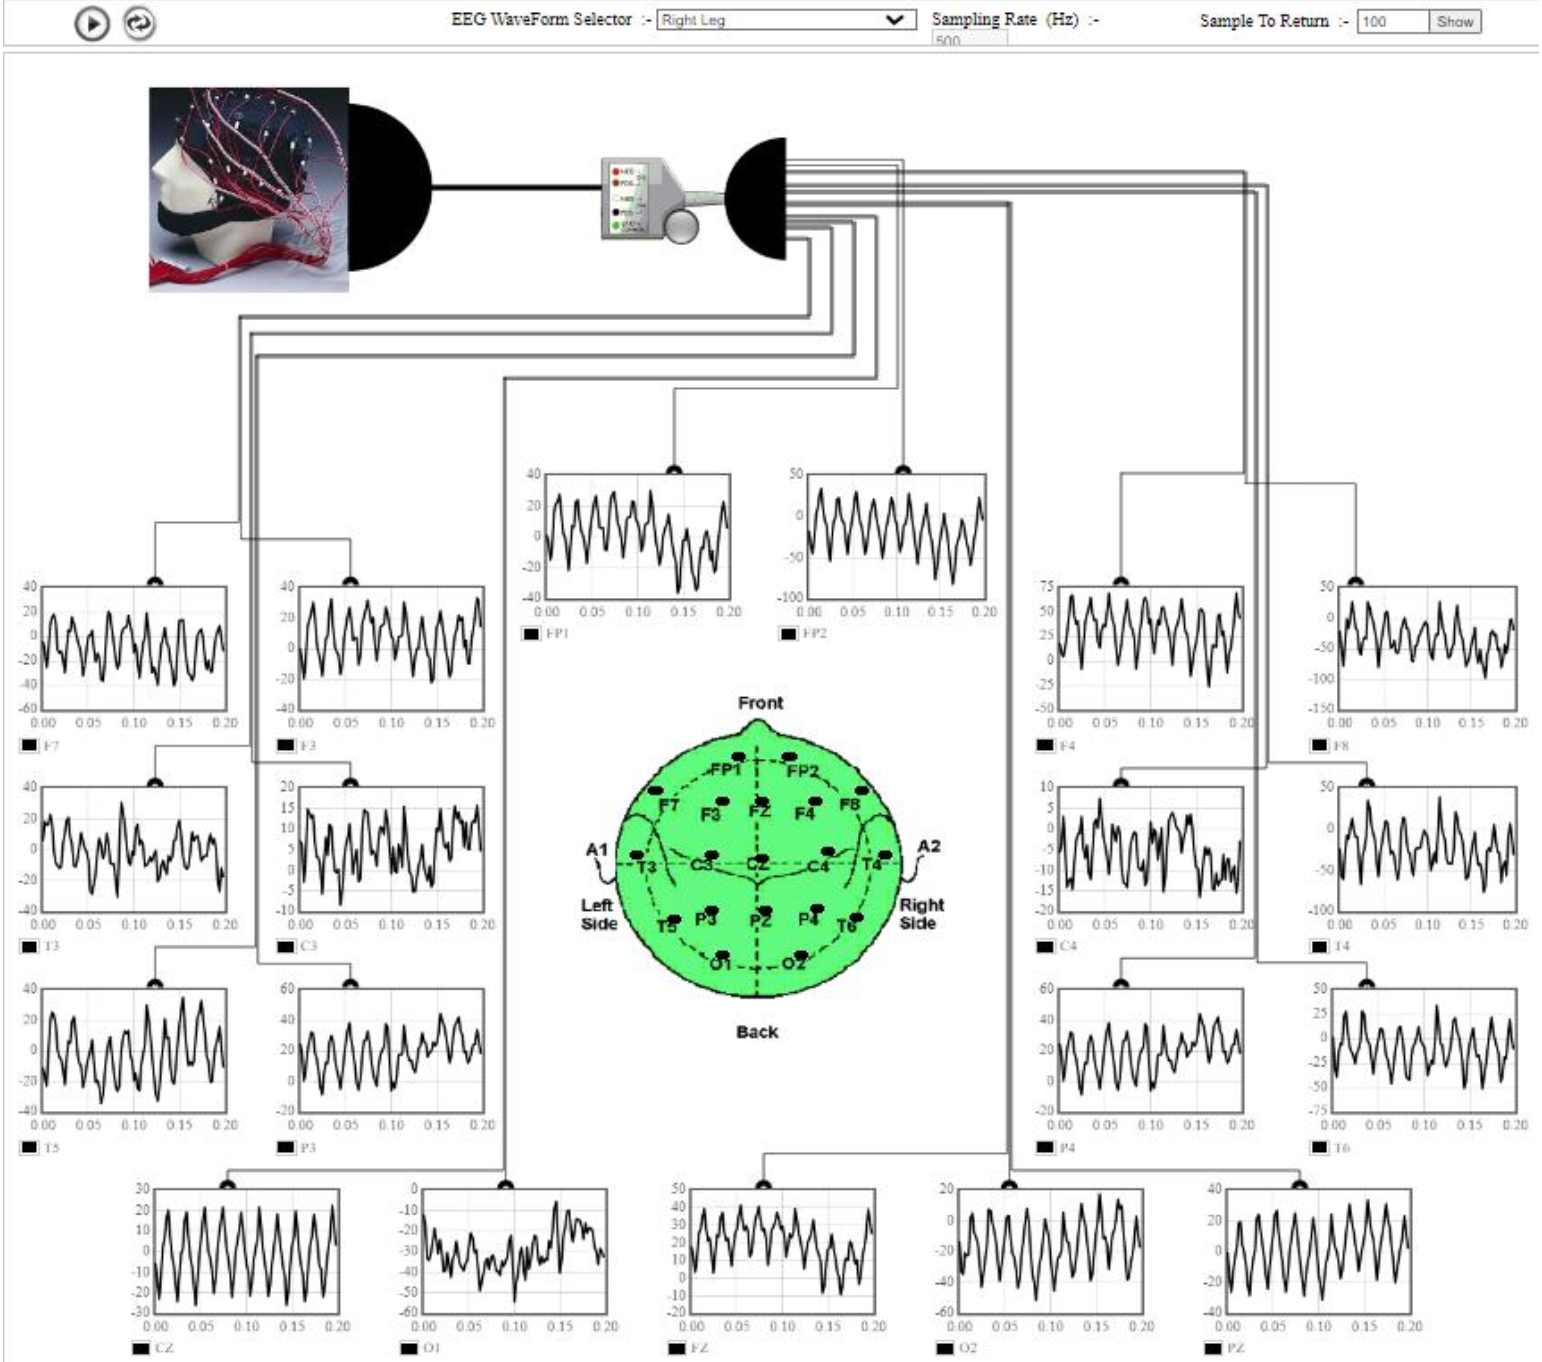
\includegraphics[width=5.70833in,height=\textheight]{images/clipboard-1649723628.png}
\end{center}

\section{Result}\label{result-5}

\begin{quote}
Thus, EEG Waveforms were simulated. Patterns were observed for movement
of different body parts.
\end{quote}

\bookmarksetup{startatroot}

\chapter{Defibrillator Waveform
Simulation}\label{defibrillator-waveform-simulation}

\section{Aim}\label{aim-7}

\begin{enumerate}
\def\labelenumi{\arabic{enumi}.}
\tightlist
\item
  To simulate the Defibrillator output waveform
\item
  To understand energy levels generated by defibrillator
\item
  To understand the necessity and applications of defibrillator
\item
  To understand various controls associated with defibrillator
\item
  To understand various configurations and types of defibrillator
\end{enumerate}

\section{Pre Requisites}\label{pre-requisites-2}

\begin{itemize}
\tightlist
\item
  Knowledge of various cardiac arrhythmias
\item
  Tools like NI LabVIEW and MATLAB
\end{itemize}

\section{Theory}\label{theory-7}

The instrument for administering the shock is called a defibrillator.
Electric shock by defibrillator is used to reestablish normal activity.
The shock can be delivered to the heart by means of electrode placed on
chest of the patient.

Ventricular fibrillation is serious cardiac emergency resulting from
asynchronous contraction of heart muscle. This uncoordinated movement of
ventricle walls of the heart may result from electric shock or from
abnormalities of body chemistry. Main problem of fibrillation is
continuously stimulation of adjacent cells of heart muscle fibers.so
there is no synchronized succession of events that follow heart action.
This Fibrillation leads to loss of cardiac output and irreversible brain
damage or death if not reversed within 5 minutes of onset.

\begin{center}
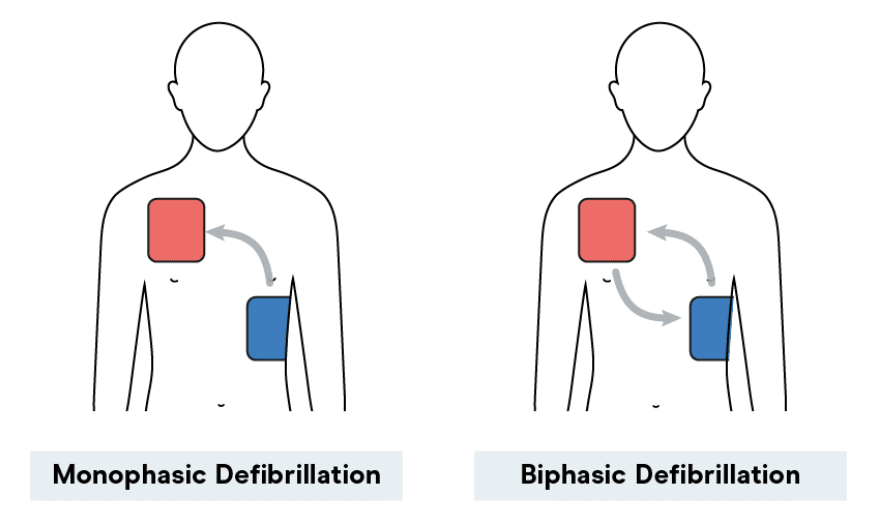
\includegraphics[width=5.03125in,height=\textheight]{images/clipboard-1102124754.png}
\end{center}

\begin{center}
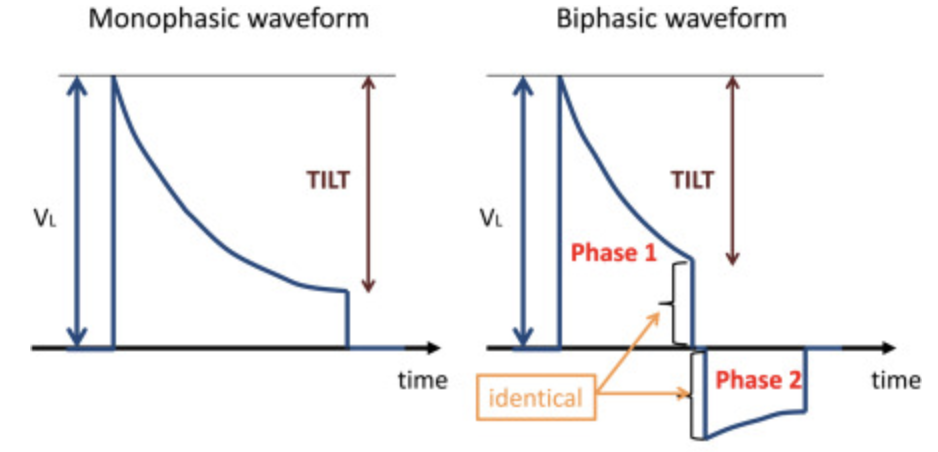
\includegraphics[width=5.03125in,height=2.34375in]{images/clipboard-1322675172.png}
\end{center}

\begin{itemize}
\tightlist
\item
  Monophasic pulse width is typically programmable from 3.0 to 12.0
  msec.
\item
  Biphasic positive pulse width is typically programmable from 3.0 to
  10.0 msec, while the negative pulse is from 1.0 to 10.0 msec
\item
  Studies suggest that biphasic pulses yield increased defibrillation
  efficacy with respect to Monophasic pulses
\item
  Monophasic pulse width is typically programmable from 3.0 to 12.0
  msec.
\item
  Biphasic positive pulse width is typically programmable from 3.0 to
  10.0 msec, while the negative pulse is from 1.0 to 10.0 msec
\item
  Studies suggest that biphasic pulses yield increased defibrillation
  efficacy with respect to Monophasic pulses
\end{itemize}

\section{Simulation}\label{simulation-2}

\begin{center}
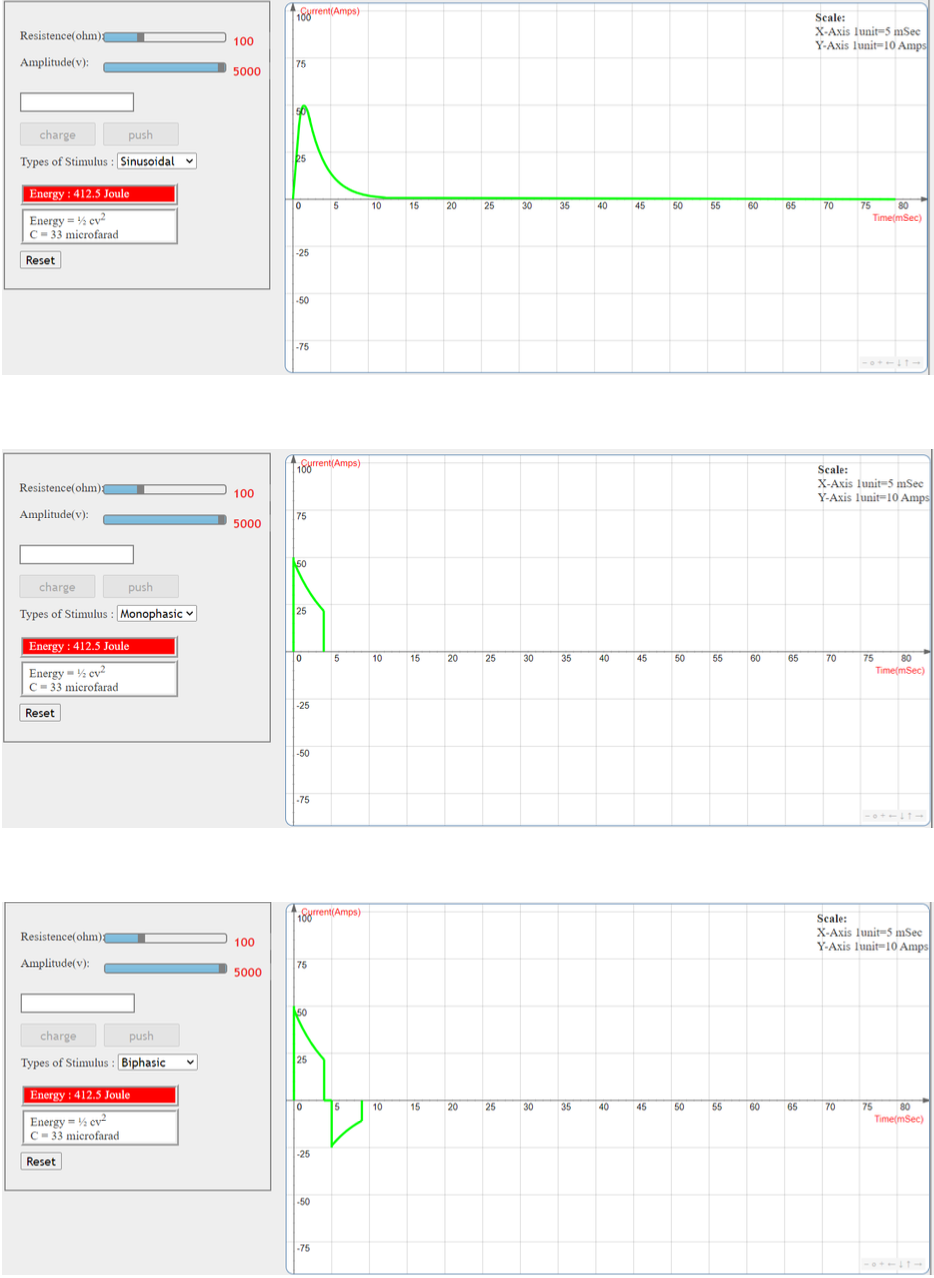
\includegraphics[width=5.375in,height=7.13542in]{images/clipboard-2000378057.png}
\end{center}

\section{Result}\label{result-6}

\begin{quote}
Thus, the output waveform of defibrillator was simulated. Monophasic and
Biphasic waveforms were observed and understood.
\end{quote}

\bookmarksetup{startatroot}

\chapter{Asynchronous and Synchronous Pacemaker Waveform
Simulation}\label{asynchronous-and-synchronous-pacemaker-waveform-simulation}

\section{Aim}\label{aim-8}

\begin{enumerate}
\def\labelenumi{\arabic{enumi}.}
\tightlist
\item
  To simulate the pacemaker output waveform
\item
  To understand various energy levels generated by pacemaker
\item
  To understand the necessity and applications of pacemaker
\item
  To understand various types and configurations of pacemaker
\item
  To understand various controls associated with the pacemaker
\end{enumerate}

\section{Pre Requisites}\label{pre-requisites-3}

\begin{enumerate}
\def\labelenumi{\arabic{enumi}.}
\tightlist
\item
  Knowledge of cardiac arrhythmias
\item
  Tools like NI LabVIEW and MATLAB
\end{enumerate}

\section{Theory}\label{theory-8}

A pacemaker is an electronic device that provides an electrical signal
to make the heart beat when it's own, built-in pacemakers fail. The
anatomical, built-in pacemakers provide what is called the ``intrinsic''
rhythm, and they can be disrupted by various conditions - ischemia for
example, or by an MI. It is prosthetic device for the heart, first
conceived in 1932 by Albert S. Hymen, an American cardiologist. In 1952
the pacemaker was used clinically by Paul M. Zoll as an external device.

Abnormality in cardiac normal rhythm is called cardiac arrhythmia. There
are various types of cardiac disorder. Some of them are Bradycardia and
tachycardia. In bradycardia heart rate goes down from normal rate
(i.e.~below 60) and in tachycardia heart rate is higher than normal
rate.

\section{Simulation of Asynchronous Pacemaker Output
Waveform}\label{simulation-of-asynchronous-pacemaker-output-waveform}

\begin{center}
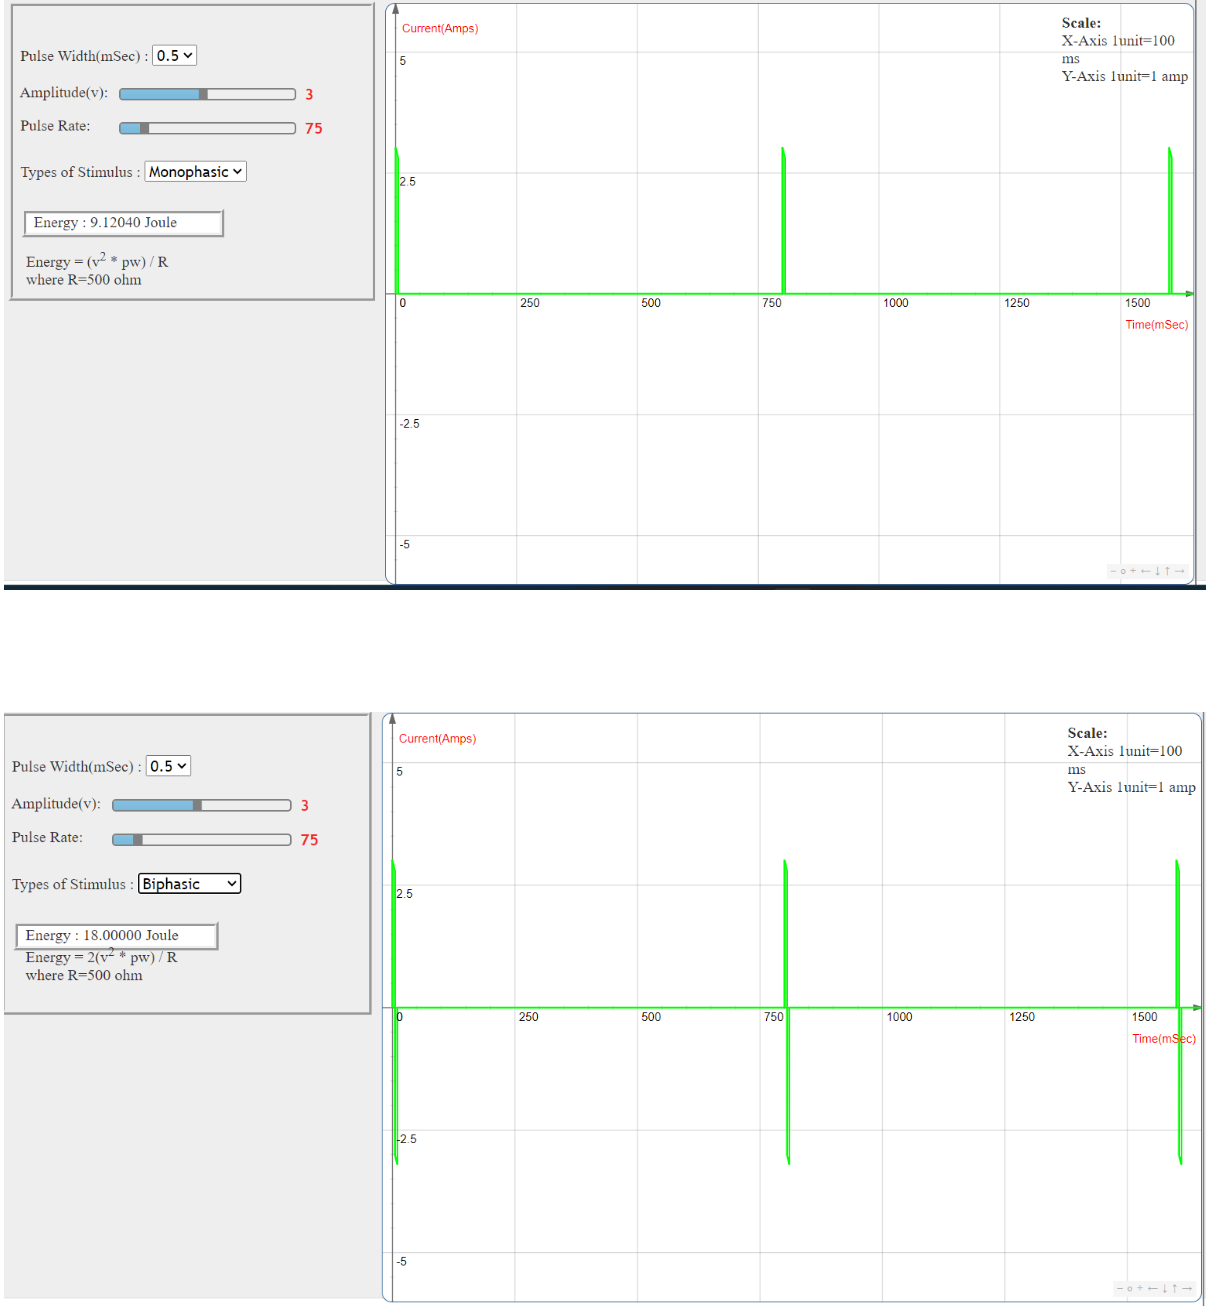
\includegraphics[width=6.07292in,height=\textheight]{images/clipboard-243054570.png}
\end{center}

\section{Simulation of Synchronous Pacemaker Output
Waveform}\label{simulation-of-synchronous-pacemaker-output-waveform}

\begin{center}
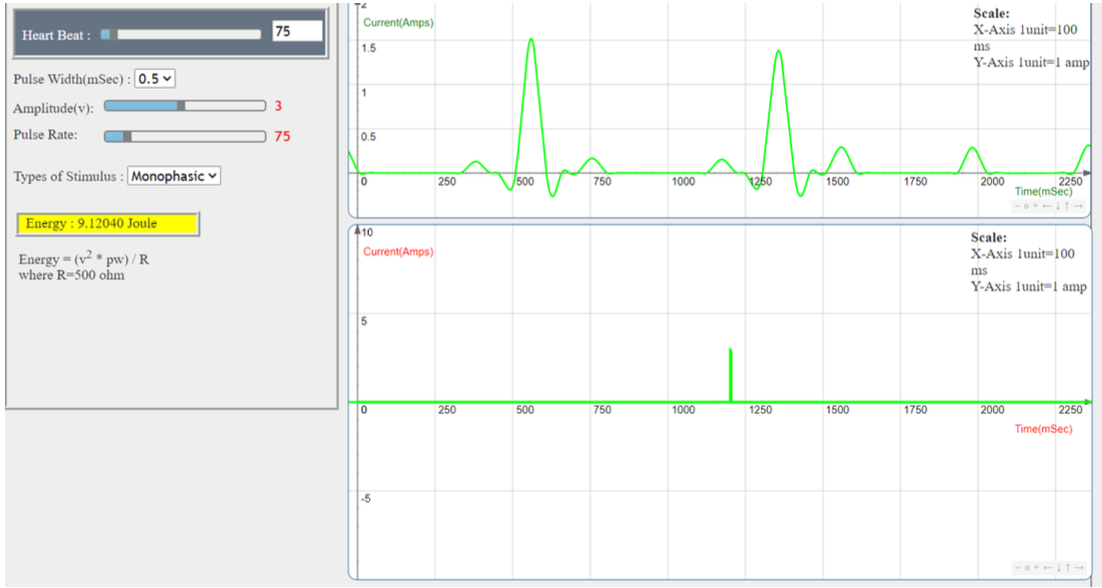
\includegraphics{images/clipboard-3780312789.png}
\end{center}

\begin{center}
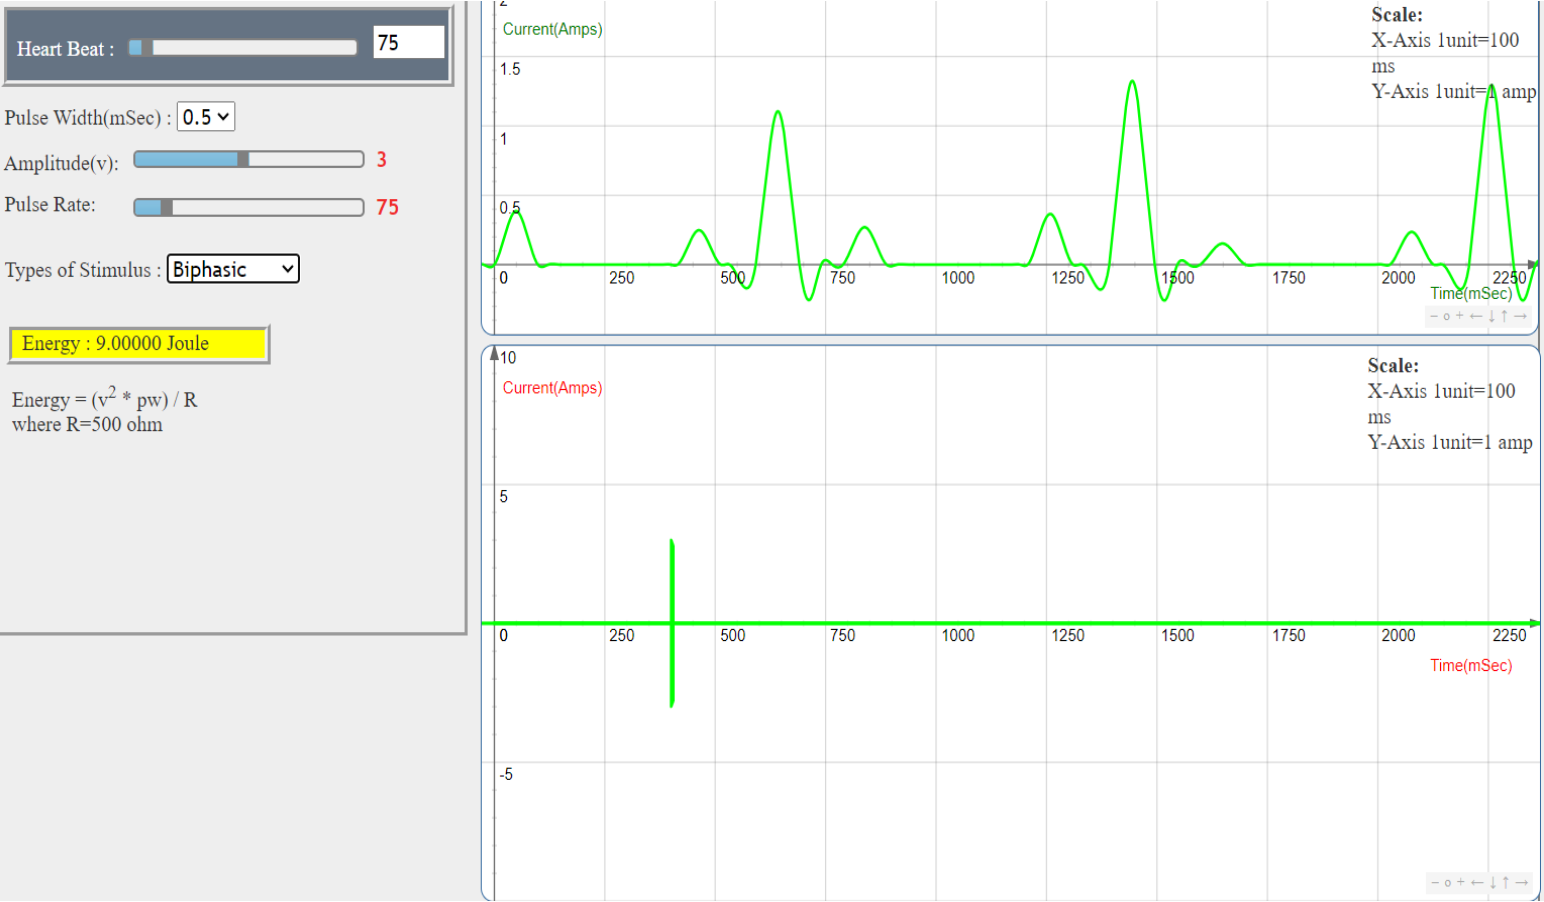
\includegraphics[width=6.04167in,height=\textheight]{images/clipboard-3757172610.png}
\end{center}

\section{Result}\label{result-7}

\begin{quote}
Thus, the waveform of the asynchronous and synchronous pacemaker was
simulated, it's configurations and controls were understood.
\end{quote}

\bookmarksetup{startatroot}

\chapter{Simulation of Hemodialysis
Machine}\label{simulation-of-hemodialysis-machine}

\section{Aim}\label{aim-9}

\begin{enumerate}
\def\labelenumi{\arabic{enumi}.}
\tightlist
\item
  To understand the block schematics / modules involved in Haemodialysis
  Machine
\item
  To understand various measurement and control involved in
  Haemodialysis Machine
\item
  To understand overall functionality of Haemodialysis Machine
\end{enumerate}

\section{Pre Requisites}\label{pre-requisites-4}

\begin{enumerate}
\def\labelenumi{\arabic{enumi}.}
\tightlist
\item
  Knowledge of physiology of Kidney
\item
  Tools like NI LabVIEW and MATLAB
\end{enumerate}

\section{Theory}\label{theory-9}

Hemodialysis means the process of filtering blood. In hemodialysis, the
filtering process takes place in a machine outside the body.
Hemodialysis is a method for removing waste products such as creatinine
and urea, as well as free water from the blood when the kidneys are in
renal failure. When the kidneys do not work well, dialysis is needed to
remove extra fluid and waste products from the body. Hemodialysis is a
type of dialysis that uses a machine with an artificial filter to remove
waste and extra fluids from the blood.

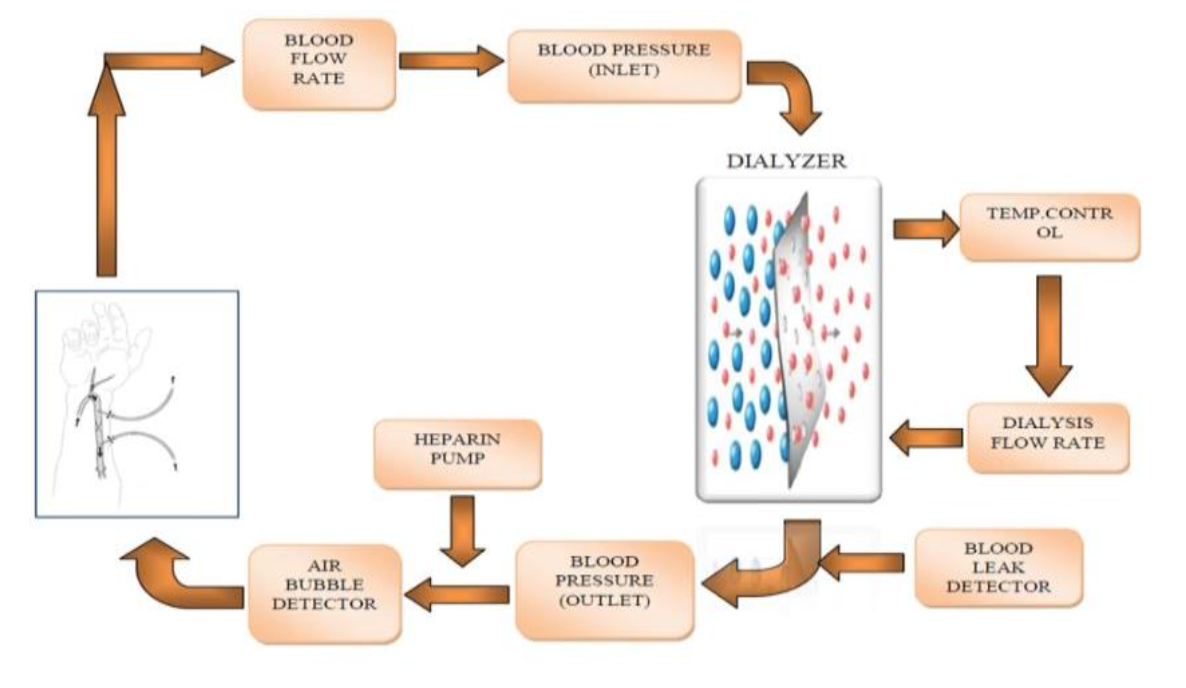
\includegraphics[width=4.34375in,height=2.65625in]{images/clipboard-2703843569.png}

\subsection{Blood flow}\label{blood-flow}

The blood pump takes and returns the blood from the patient via the
arterial and venous needles respectively. The blood is confined to the
disposable plastic tubing and doesn't come in contact with any part of
the machine. The blood coming from the pump flows to the dialyzer and
the blood that leaves the dialyser returns to the patient through the
venous needle. The pump speed, and the resulting blood flow rate, is
adjustable from zero to about 600 cc/min. While pump speed is
controlled, blood flow rate is displayed. These two usually go hand in
hand, but not always. The blood flow rate is calculated based on the
pump RPM (revolution per minute), and the diameter of the tube. The
calculated blood flow is displayed. The control doesn't check the real
blood flow. It displays blood flow even if the pump turns without the
plastic tube installed.

The real blood flow may differ from the display because of:

\begin{itemize}
\tightlist
\item
  \emph{Internal reverse leak:} the rollers never squeeze the tube
  completely so not all the blood is pushed forward, a little goes
  backward.
\item
  High arterial and/or venous pressure reduces the ability of the pump
  to suck or to deliver.
\item
  Any speed above some low value gradually reduces the blood flow. For a
  display of 600 cc/min the actual blood flow is 500 or less. In
  addition to the inherent features of the pump, a human error that may
  reduce blood flow is the way the plastic tube is installed in the
  pump. If the plastic tube inside the pump is too tight it cannot
  expand to its full volume, so the suction is reduced, and the pump
  delivers less blood flow than the display indicates.
\end{itemize}

\section{Blood pressure}\label{blood-pressure}

The blood pressure is measured both when it taken out from the limb and
also when it is returned.

\subsection{Arterial \& Venous Pressure}\label{arterial-venous-pressure}

These pressures are the result of the blood forced to flow through the
plastic tubing, the dialyzer, and the needles.

\subsection{Arterial pressure}\label{arterial-pressure}

When the blood flow rate increases the arterial pressure becomes more
negative. If it is too negative the red blood cells may break down. This
is called hemolysis. To be on the safe side never let the arterial
pressure go below -220 mmHg. If it goes below that the pump speed should
be reduced. If your blood count is low you may notice that the pump
speed should be reduced as your blood count goes up.

\subsection{Blood flow rate}\label{blood-flow-rate}

The effect of blood flow is easy to follow - any change in pump speed is
immediately reflected on the pressure displays. The higher the flow the
higher the pressure.

\subsection{Dialysis Process}\label{dialysis-process}

Concerning the blood, dialysis performs 2 different functions that are
normally done by healthy kidneys: - Removing excess fluid. - Removing
waste like urea, and excess electrolytes (chemicals) like potassium,
magnesium, sodium, etc.

The dialysis is performed inside the dialyzer, which is a plastic
cylinder, in which the blood enters from the top, flows through
thousands of extremely thin hollow fibers and leaves from the bottom. At
the same time the dialysate enters from the bottom, flows around and in
between the fibers, and leaves from the top. The fibers are semi
permeable membranes, that is, smaller molecules in the blood stream can
pass through them into the dialysate and bigger molecules as well as
blood cells cannot. Dialysate is a water-based solution and its purpose
is to absorb from the blood all that should be removed and nothing else.

Waste and electrolytes move from the blood into the dialysate because
their concentration in the blood is higher. This process is called
diffusion. The dialysate flow ensures that fresh dialysate is present at
all times so that the dialysate doesn't become saturated, and the
process never ends.

Fluid is removed from the blood in the same way the kidneys do it - by
blood pressure. This process is called Ultra Filtration (UF) and is
similar to Reverse Osmosis (RO). With RO, the membrane pore size is very
small and allows only water to pass through the membranes. In UF, the
membrane pore size is larger, allowing some bigger molecules to pass
through the pores with the water.

The rate at which fluid is removed from the blood is called UFR (UF
Rate). There is higher pressure in the blood passing through the
dialyzer and lower pressure in the dialysate. This pressure difference
is called TMP (Trans Membrane Pressure). The higher the TMP the higher
the UFR.

The rest of the machine takes care of supplying the blood and the
dialysate to the dialyzer, controls the flow and the pressures, and
provides visual indication and alarm when something goes wrong.

\subsection{Dialysate}\label{dialysate}

The dialysate is a water-based solution. With all contemporary machines,
the dialysate concentrate is fed into the machine, water is fed from a
water tank and a marvelous pump mixes them to the desired concentration.
- Calcium (Ca) can be 3.5, 2.5, 2 mEq/L, depending upon the patient's
calcium. (US units; Ca 3.5 mEq/L equal 1.75 mmol/L). - Potassium (K) can
be 4, 3, 2, 1 mmol/L, or zero (free-K). (US units, used
internationally).

\subsection{Dialysate flow}\label{dialysate-flow}

The dialysate pump, in addition to mixing the concentrate with water,
moves the dialysate through the dialyzer. This pump has an adjustable
flow rate. For regular dialysis at blood flow up to 250 cc/min the
dialysate flow should be 500 cc/min. For more efficient dialysis, called
high flux, the blood flow is 400-500 cc/min, and the dialysate flow is
800 cc/min. In addition to controlling the flow, this multi-function
pump controls the pressure of the dialysate as to achieve the desired
TMP and hence the desired UFR.

\subsection{UF and UFR}\label{uf-and-ufr}

In modern dialysis machines either UF or UFR can be set. When UF is set
it is called Goal; that's how many grams or cc of fluid to remove.
Treatment time should also be entered so the control can calculate the
UFR and the TMP. This is the way it is done in most centers. The control
is sophisticated enough to recalculate the UFR if the goal is changed
during the treatment.

\subsection{Blood Leak}\label{blood-leak}

Blood may leak inside the dialyzer because of ruptured fibers. This may
happen even with a new dialyzer. There could be a minor leak, which is
invisible, or a major leak in which blood can be seen in the dialyzer.
In both cases the machine stops and sets the alarm. To resume dialysis
the dialyzer should be replaced.

\subsection{Heparin Pump}\label{heparin-pump}

This pump delivers heparin to the blood tubing. The pump is a regular
syringe that is pushed by a controlled motor. On all machines the rate
can be adjusted. Usually an initial dose of heparin is given when the
treatment begins, then the pump delivers heparin until one hour before
the end. All patients need continuous heparin.

In case of a patient after surgery or another kind of bleeding, heparin
is used sparingly or not at all. To avoid clotting in the dialyzer it is
rinsed with 100 cc saline every hour or so. In spite of that, the blood
in the dialyzer may clot, but unless the patient has a very low blood
count no treatment is required (of course the heparin dose should be
increased when possible).

\subsection{Temperature}\label{temperature}

To make it more convenient for the patient, the dialysate temperature
can be set to a desired value, so the blood returning to the patient
will not be too cold. For most patients a setting of 37 C (98.6 F) is
ok.

\subsection{Treatment Time}\label{treatment-time}

Each treatment takes about 4 hours and is done three times each week.
Moreover, depending upon the patient's clinical history the treatment
may vary.

\subsection{Alarm}\label{alarm}

There is a red alarm light. There are many reasons for the machine to
alarm: the reason is either Air bubble detection or Blood leak
detection.

\section{Simulation}\label{simulation-3}

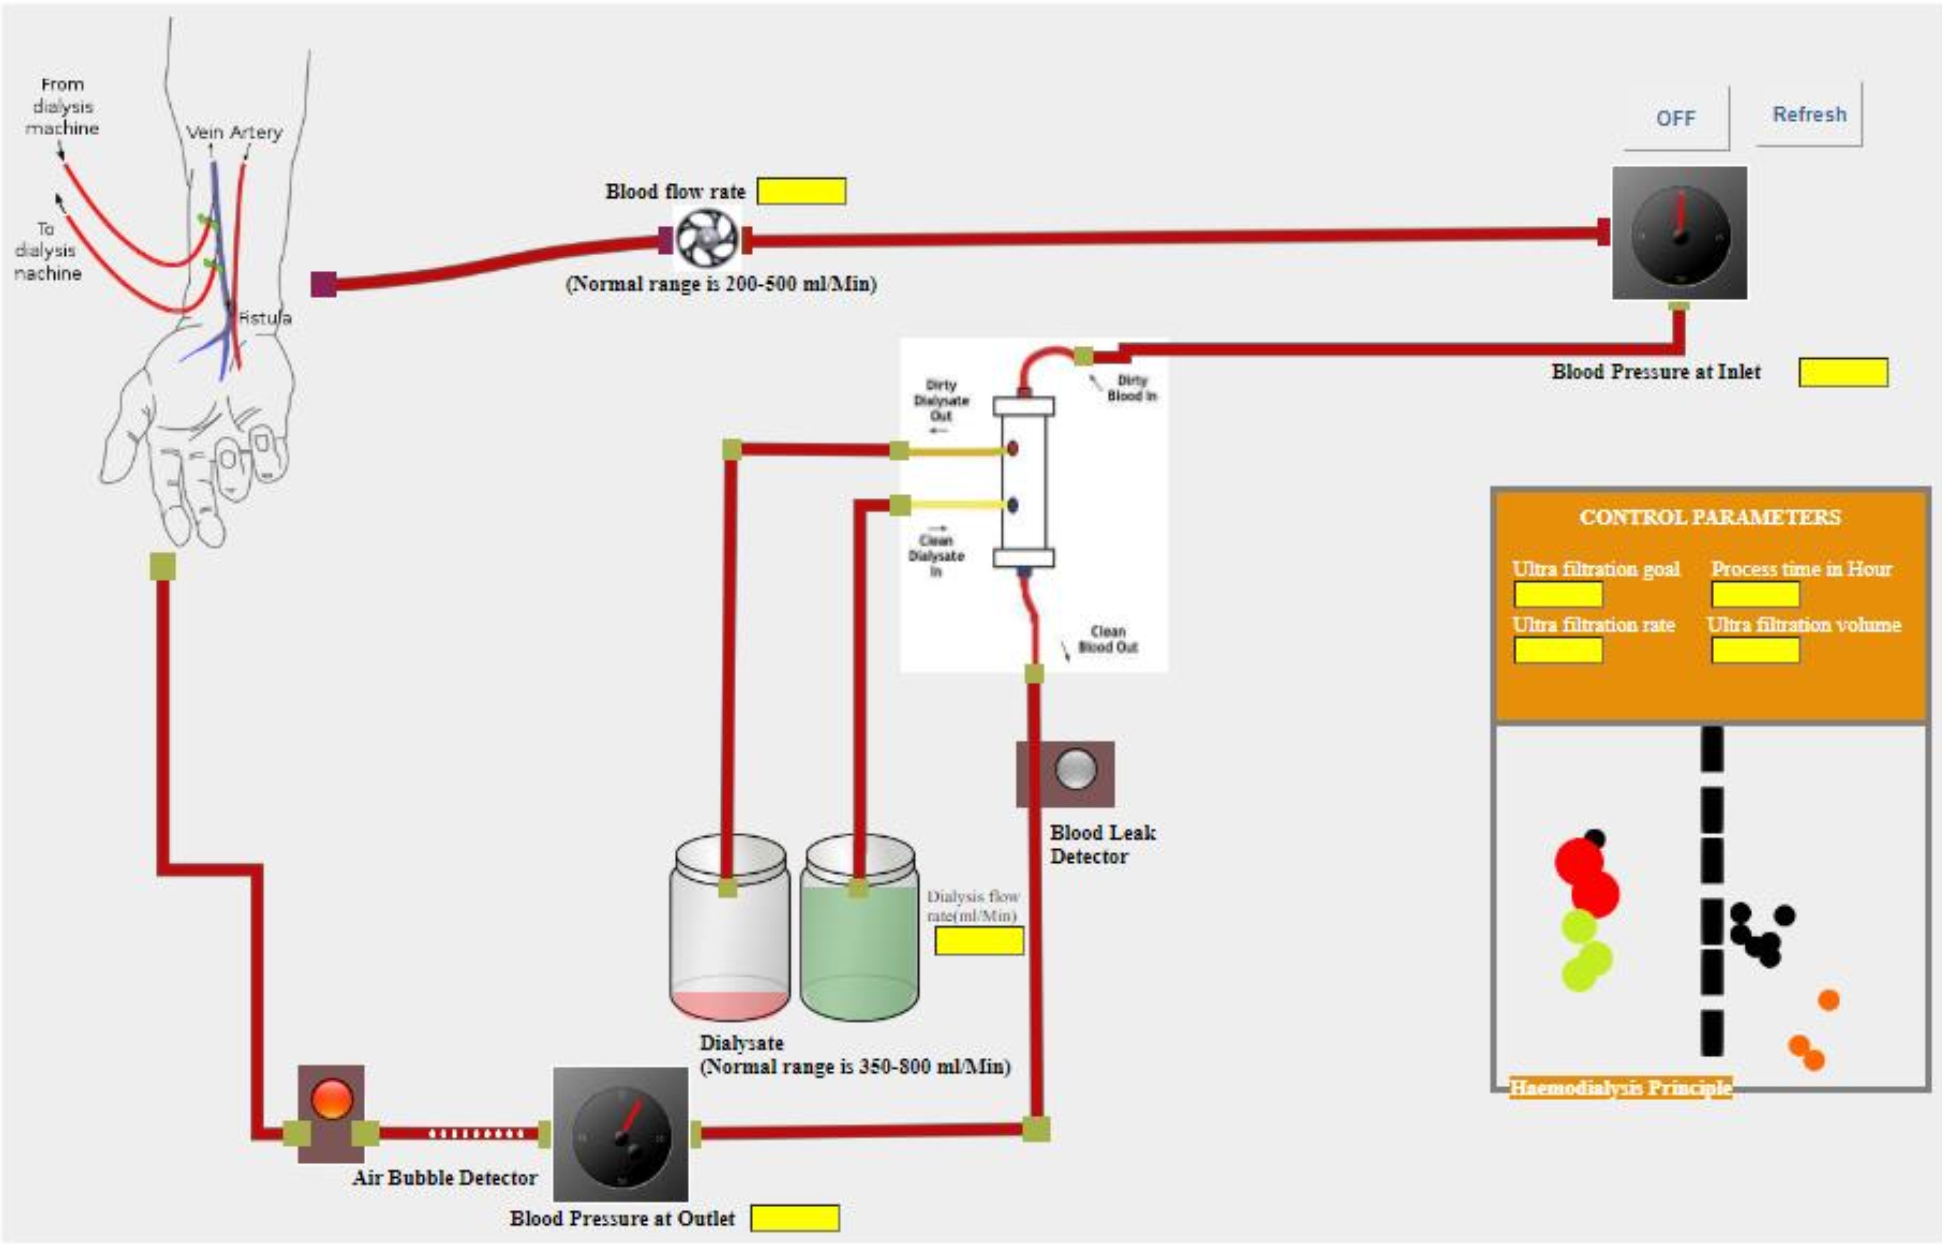
\includegraphics[width=6.04167in,height=\textheight]{images/clipboard-2890244601.png}

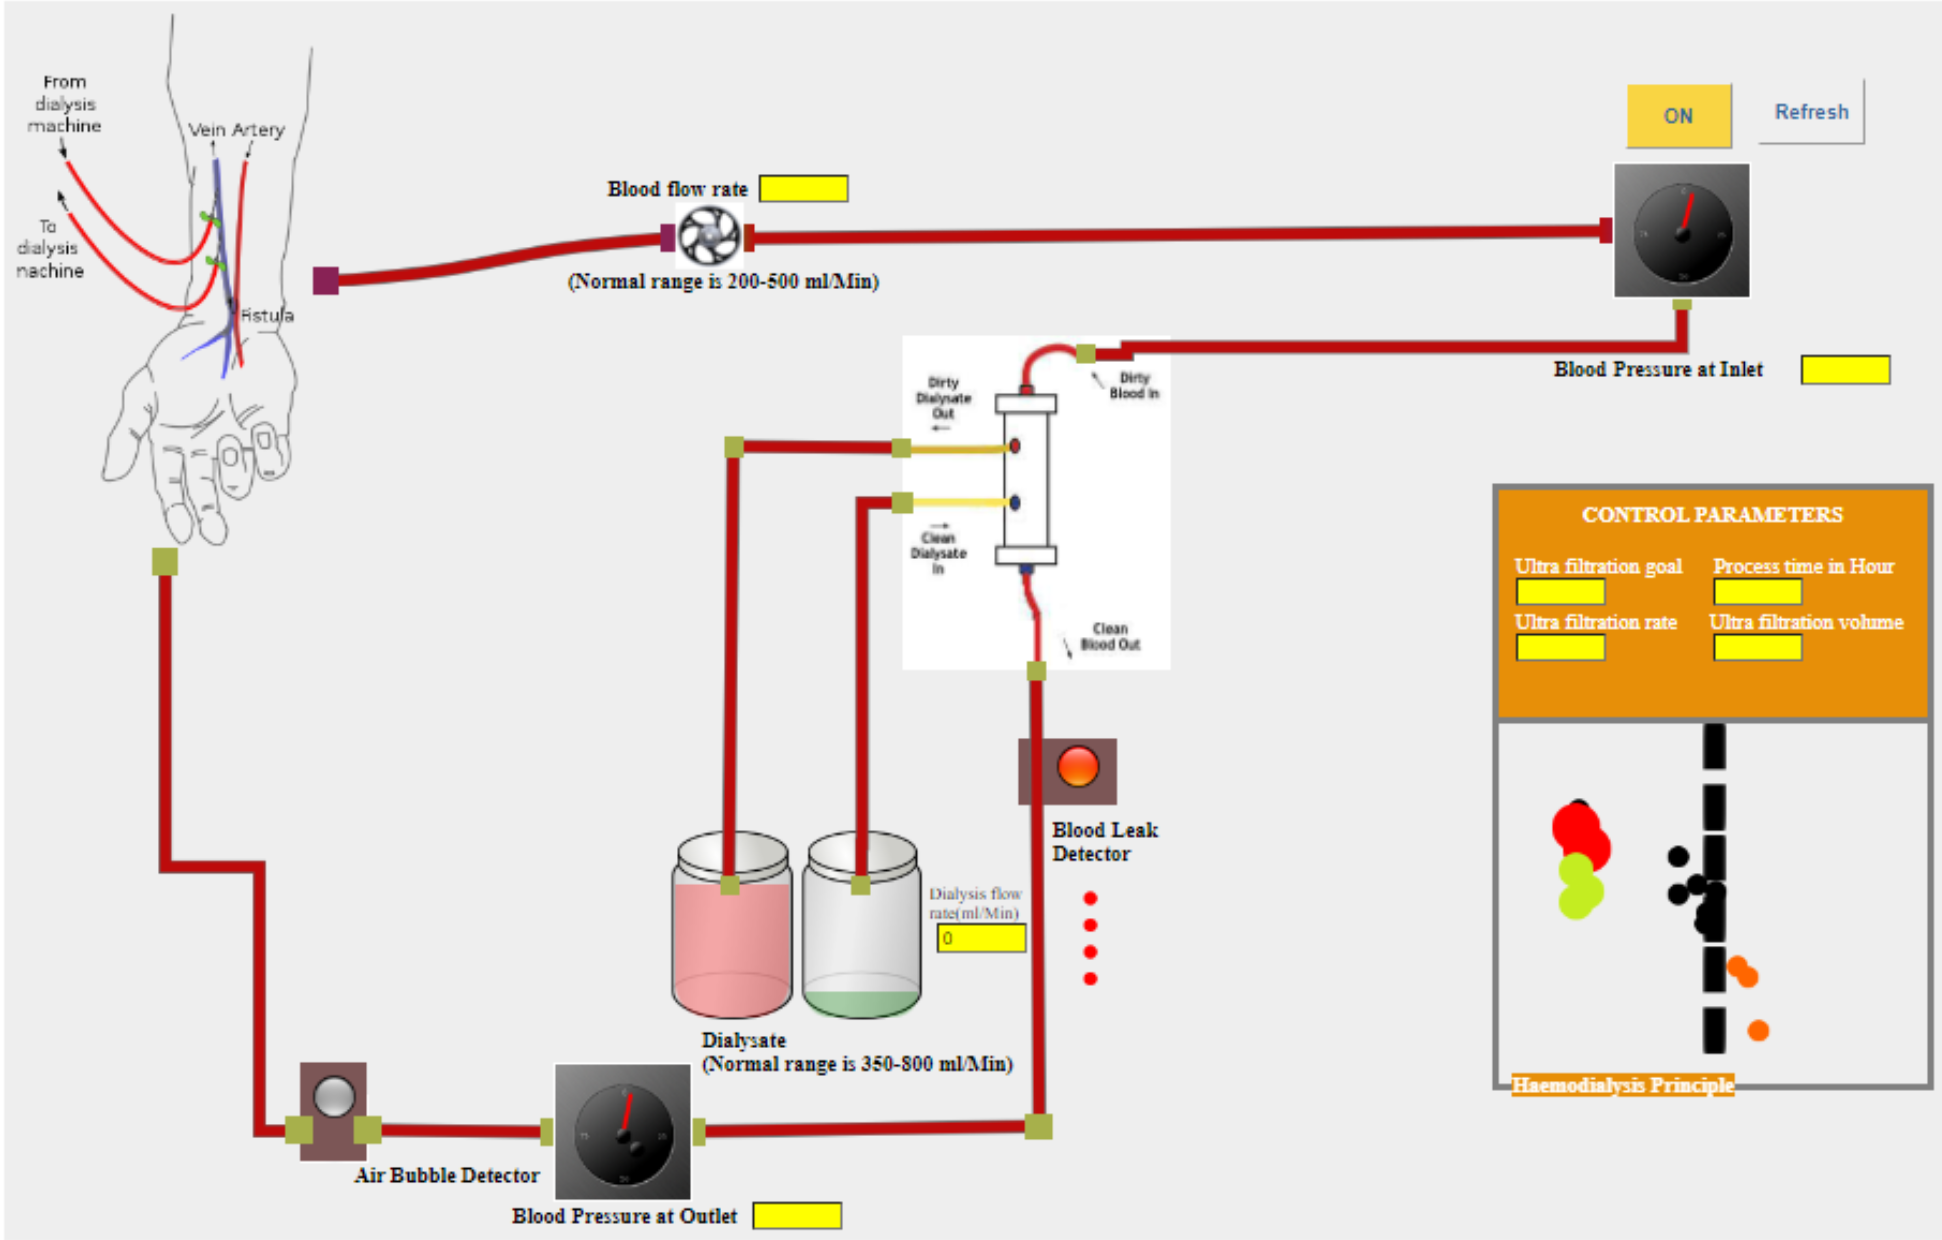
\includegraphics[width=6.01042in,height=\textheight]{images/clipboard-3169178804.png}

\section{Result}\label{result-8}

\begin{quote}
Thus, the simulation of the hemodialysis machine is working, and the
output was studied.
\end{quote}



\end{document}
